\documentclass[10pt, a4paper]{report}
%====================== PACKAGES ======================

\usepackage[french]{babel}
\usepackage[utf8]{inputenc}
\usepackage{float}
\usepackage{amsmath}
\usepackage{graphicx}
\usepackage[colorinlistoftodos]{todonotes}
\usepackage{url}
\usepackage{hyperref}
\usepackage{array}
\usepackage{tabularx}
\usepackage{setspace}
\usepackage{abstract}
\usepackage[T1]{fontenc}
\usepackage[a4paper, top=2cm, bottom=2cm, left=2cm, right=2cm]{geometry}
\usepackage{subfig}
%\usepackage{tocloft}
\usepackage{listings}
\usepackage{xcolor}
\usepackage{titlesec}

%====================== CONFIGURATION ======================
\titleformat{\section}{\LARGE\bfseries}{\thesection}{1em}{}
\titleformat{\subsection}{\Large\bfseries}{\thesubsection}{1em}{}
\titleformat{\subsubsection}{\Large\bfseries}{\thesubsubsection}{1em}{}


%====================== INFORMATION ET REGLES ======================

%rajouter les numérotation pour les \paragraphe et \subparagraphe
\setcounter{secnumdepth}{4}
\setcounter{tocdepth}{4}

\hypersetup{
pdfauthor = {AYEVA Yaasin},			% Auteurs
pdftitle = {Rapport de Stage Fixaars, JS Morlu Ghana},	
pdfsubject = {Stage de fin d'études},
pdfstartview={FitH},
pdfcreator = {OverLeaf - TeX Live 2023},% Logiciel qui a crée le document
pdfproducer = {Yaasiin.dev}
}

%======================== DEBUT DU DOCUMENT ========================

\begin{document}
%régler l'espacement entre les lignes
\newcommand{\HRule}{\rule{\linewidth}{0.8mm}}
%page de garde
\begin{titlepage}
\begin{center}

% Upper part of the page. The '~' is needed because only works if a paragraph has started.

\includegraphics[width=0.35\textwidth]{assets/presentation/ifnti}~\\[1cm]

{\fontsize{13.5pt}{10pt}\selectfont
\textsc{Institut de Formation aux Normes et Technologies de l'Informatique}
}\\[1cm]

\textsc{\Large }\\[0.5cm]

% Title
\HRule \\[0.4cm]

{\huge \bfseries 
Rapport de stage de fin d’études \\ Stage effectué du 29/01/2024 au 28/06/2024 \\
Réalisation d’une application de mise en relation de prestataires de services locaux - Fixaars\\[0.4cm] }


\HRule \\[1.5cm]

% Author and supervisor
\begin{minipage}{0.4\textwidth}
\begin{flushleft} \large
\emph{Auteur:}\\
Yaasiin \textsc{Ayeva}\\
% \textsc{IDRISSOU Djabir}
\end{flushleft}
\end{minipage}
\begin{minipage}{0.4\textwidth}
\begin{flushright} \large
\emph{Entreprise d'accueil:} \\
JS Morlu Ghana \textsc{}\\
\emph{Superviseur:} \\
Aliloulaye \textsc{Tchaou}
\end{flushright}
\end{minipage}

\vfill

% Bottom of the page
%{\large \today}
{\large 29 janvier 2024}

\end{center}
\end{titlepage}
%page blanche
\newpage
~
%ne pas numéroter cette page
\thispagestyle{empty}
\newpage

\renewcommand{\abstractname}{Remerciements}
\renewcommand{\abstractnamefont}{\normalfont\Large\bfseries}
\renewcommand{\abstracttextfont}{\normalfont\Large}
\begin{abstract}
\begin{spacing}{1.37}

L’achèvement de ce projet n’aurait pas été possible sans le soutien de nombreuses personnes.

Une profonde gratitude est adressée à la famille, dont les sacrifices et le soutien constant ont contribué de manière décisive à la réussite de ce parcours.

Les remerciements vont également à M. Aliloulaye TCHAHOU, pour la confiance, la patience et l’encadrement apportés tout au long de cette expérience, ainsi qu’à M. Mohammed SOWOU, pour ses conseils avisés et son accompagnement.

La solidarité des camarades de promotion a joué un rôle fondamental, de même que l’implication du personnel de l’IFNTI-Sokodé, en particulier M. Sabirou TÉOURI, Directeur de l’institut, pour son soutien.

Les enseignants, notamment Jean-Christophe Samuel CARRÉ, François DECQ, Willy AUBRY et Kokou Wama DJIMISSA, sont également remerciés pour leur engagement pédagogique.

Enfin, un remerciement particulier est adressé à l’équipe de JS Morlu pour l’accueil et la disponibilité manifestés durant le stage.

\end{spacing}
\end{abstract}

\newpage
\thispagestyle{empty} \vspace*{\fill}
\begin{flushright}
    \textit{\textbf{“La simplicité est la sophistication ultime."} } \\
    \textit{car il faut une compréhension profonde et une réflexion rigoureuse} \\
    \textit{pour transformer quelque chose de complexe en une solution élégante et facile à utiliser.} \\ \vspace{0.25cm}
    -- Léonard de Vinci.
\end{flushright}
\vspace*{\fill}
\newpage

{\Large
\tableofcontents
}
\thispagestyle{empty}
\setcounter{page}{0}

\newpage

\renewcommand{\baselinestretch}{1.37}
%espacement entre les lignes d'un tableau
\renewcommand{\arraystretch}{2.0}

%====================== INCLUSION DES PARTIES ======================

~
\thispagestyle{empty}
%recommencer la numérotation des pages à "1"
\setcounter{page}{0}
\newpage

{\fontsize{18pt}{18pt}\selectfont

\chapter*{Introduction}
La formation en Informatique des Organisations à l’Institut de Formation aux Normes et Technologies de l’Informatique (IFNTI) prévoit un stage de fin d’études. Ce stage permet d'appliquer les compétences acquises et de se préparer à la vie professionnelle. Ce stage, d'une durée de six mois, m'a permis de me familiariser avec un contexte professionnel réel.

Mon stage s'est déroulé au sein de JS Morlu, située à East Legon, Accra (Ghana), sous la supervision de M. Aliloulaye Tchaou, Développeur Senior au département IT. Mon projet principal a consisté à développer une application web et mobile pour mettre en relation des prestataires de services locaux. Cette mission visait à enrichir le portefeuille de projets IT de l'entreprise et à proposer une solution pratique à la communauté locale.

Ce stage s'est principalement déroulé en télétravail, favorisant ainsi les collaborations et les réunions en ligne. Cette modalité a facilité mon intégration et le suivi du projet, tout en reflétant les pratiques modernes du travail à distance.

Ce rapport est structuré en trois parties : présentation de JS Morlu Ghana, description détaillée du projet de développement et enfin, présentation des travaux réalisés, des détails techniques, des défis rencontrés et des solutions apportées. Ce document vise à retracer mon apprentissage et mes contributions durant ce stage.

\chapter{Présentation de l'entreprise d'accueil}
\section{Description}

JS Morlu est une entreprise spécialisée dans la comptabilité et l'audit, dont le siège social est situé en Virginie (États-Unis). Elle s'est développée sur plusieurs continents, notamment en Afrique, avec des succursales au Ghana, en Gambie et au Kenya. En tant que société internationale, JS Morlu possède une équipe multiculturelle composée de collaborateurs provenant d'Asie, d'Afrique et d'Amérique.

\vspace{0.5cm}

Cette diversité culturelle enrichit sa capacité à offrir des solutions adaptées aux contextes locaux tout en respectant les normes internationales. L'objectif principal de JS Morlu est d'aider les entreprises à maximiser leur potentiel et à maintenir une croissance durable dans un environnement de plus en plus concurrentiel.

\vspace{0.5cm}

Les services spécifiques offerts par JS Morlu comprennent :

\vspace{0.3cm}

\begin{itemize}
    \item \textbf{Services traditionnels (comptabilité, fiscalité et audits)} : Tenue des comptes, gestion de la fiscalité, audit financier.

\vspace{0.3cm}

\item \textbf{Audit interne et assistance à la préparation des audits} :
Établissement de systèmes d'audit interne robustes, assistance pour la conformité aux normes financières.

\vspace{0.3cm}

\item \textbf{Redressement d'entreprise} :
Analyse de la situation, mise en place de stratégies de redressement (réorganisation financière, ajustement des coûts, recherche de nouvelles sources de revenus).

\vspace{0.3cm}

\item \textbf{Distribution de solutions informatiques} :
Solutions logicielles pour la gestion financière et les ressources humaines.

\vspace{0.3cm}

\item \textbf{Gestion des risques d'entreprise} :
Identification des vulnérabilités, mise en œuvre de plans d'atténuation.

\end{itemize}

\vspace{0.5cm}

La succursale qui m'a accueilli est située à Accra (Ghana), à Lagos Avenue, dans le quartier d'East Legon, près de la Nubuke Foundation. 

\begin{figure}[H]
\begin{center}
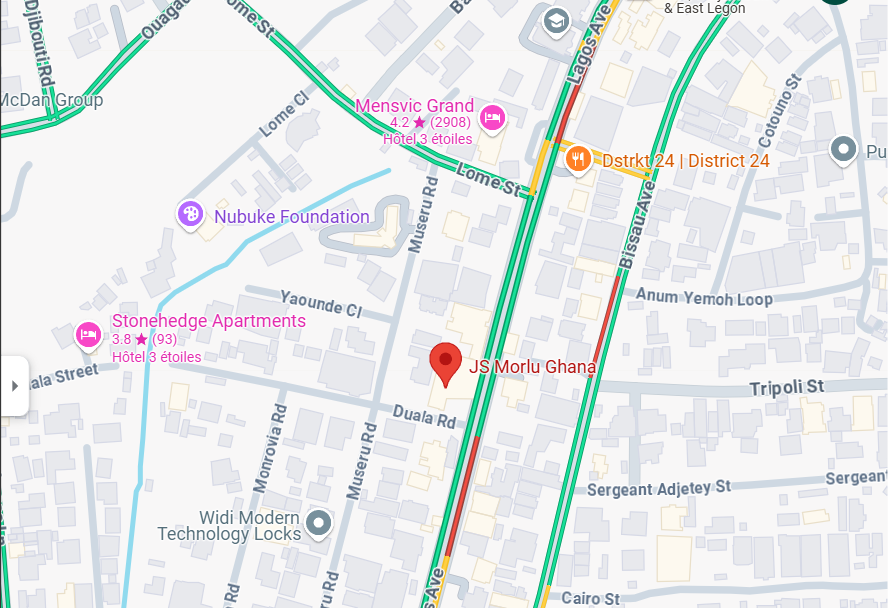
\includegraphics[width=15cm]{assets/presentation/jsmorlu-map.png}
\end{center}
\caption{JS Morlu Ghana, localisation Google Maps }
\end{figure}

\vspace{0.5cm}

Cette antenne compte une douzaine de professionnels (comptables, auditeurs et développeurs) sous la direction de M. Bernard Bempong, Directeur Général de la succursale. Mon stage s'est passé sous la supervision de M. \textbf{ Aliloulaye Tchaou}, responsable du département Ingénierie Logicielle à JS Morlu et développeur senior au sein de l'équipe.

\section{Organigramme}

L’organigramme ci-dessous illustre les principales fonctions de direction et la répartition des responsabilités au sein de JS Morlu Ghana.

\begin{itemize}
    \item En tête de l'organigramme nous avons le  \textbf{CEO (Chief Executive Officer)} M. \href{https://jsmorlu.com.gh/our-team/john-sembe-morlu-ii/}{John Sembe Morlu II}. Il est responsable de la vision stratégique globale de l’entreprise et supervise l’ensemble des activités.

    \item Ensuite vient le \textbf{DG (Directeur Général)} Monsieur \href{https://jsmorlu.com.gh/our-team/bernard-bempong/}{Bernard BEMPONG} qui coordonne les opérations et s’assure du bon fonctionnement des différents départements sous sa direction.

    \item Au même niveau de la hiérarchie, nous avons le \textbf{COO (Chief Operating Officer)}, Me \href{https://jsmorlu.com.gh/our-team/gbadee-kanteah/}{Gbadee KANTEAH}. Elle gère les opérations courantes de l’entreprise, en veillant à leur efficacité et à leur alignement avec les objectifs stratégiques.

    \item Puis, sous la supervision du DG, vient le poste de \textbf{CFO \& Services Comptables} endossé par M. \href{https://jsmorlu.com.gh/our-team/sylvester-ofori/}{Sylvester OFORI}. Ce dernier est chargé des finances et des services comptables, incluant la gestion budgétaire et la comptabilité.

    \item Au même niveau de la hiérarchie, nous avons l'\textbf{Ingénierie Logicielle \& Innovation IT} assurée par M. \href{https://jsmorlu.com.gh/our-team/aliloulaye-tchaou/}{Aliloulaye TCHAOU}. Il est responsable du développement logiciel et de l'innovation technologique adaptées aux besoins de l’entreprise et de ses partenaires.
\end{itemize}

\vspace{0.5cm}

Voici ci-dessous le visuel donnant la vue d'ensemble sur l'organigramme de JS Morlu Ghana. \\

\begin{figure}[H]
\begin{center}
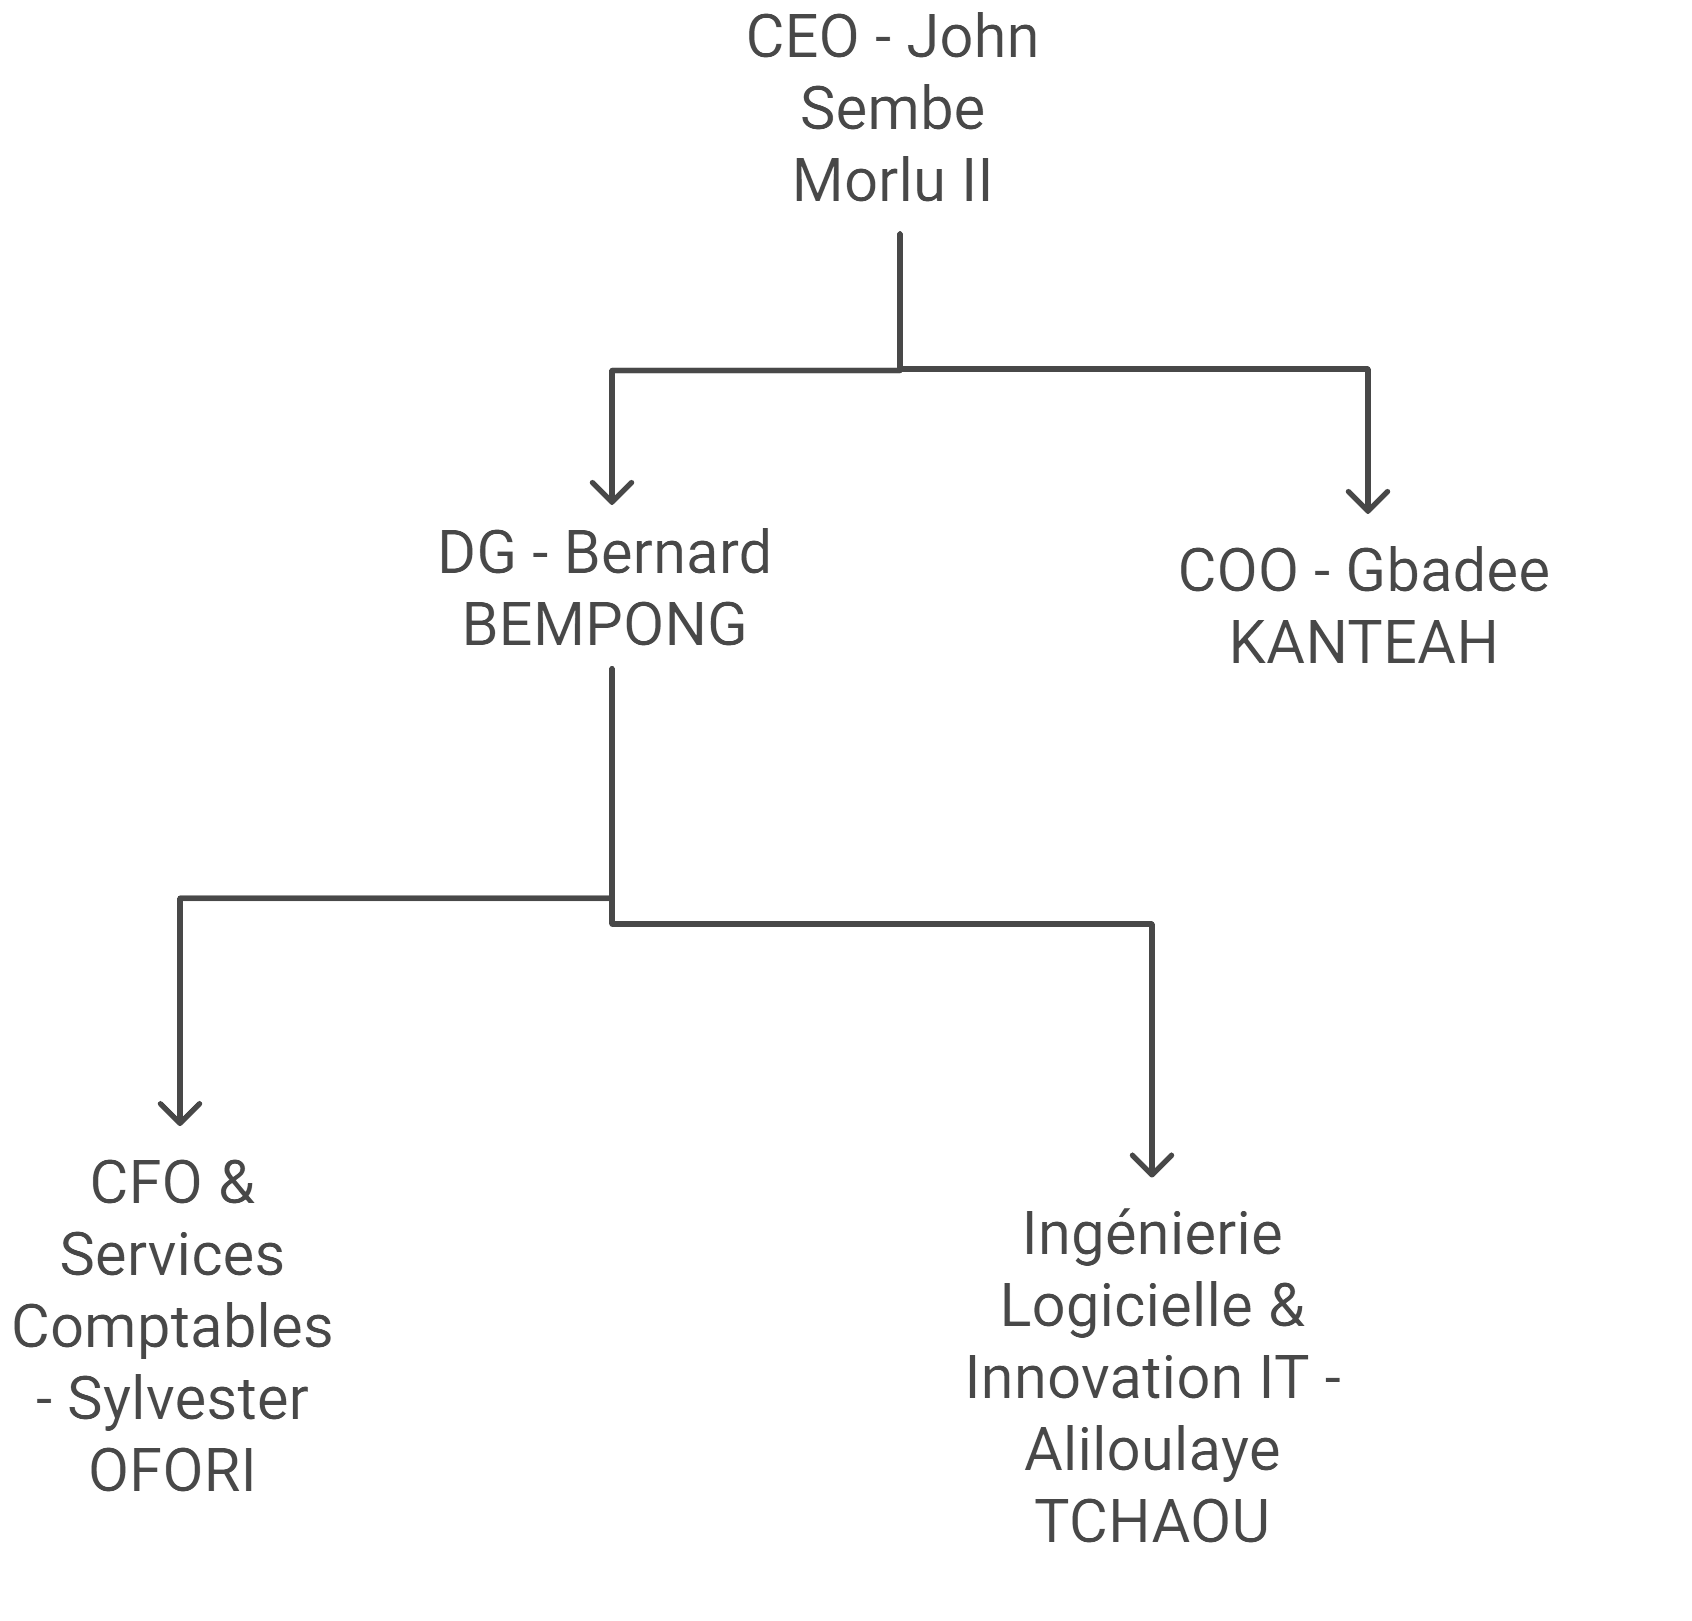
\includegraphics[width=15cm]{assets/presentation/2_organigramme.png}
\end{center}
\caption{JS Morlu Ghana, Organigramme }
\end{figure}


\section{Méthode de travail}

Afin de collaborer efficacement avec les diverses équipes impliquées dans l'implémentation des solutions, il est important de définir une méthode de travail. Pour garantir des résultats optimaux dans un environnement de développement aussi dynamique, JS Morlu a adopté la \textbf{méthode Agile} et très peu de \textbf{méthode Waterfall} ou \textbf{methode en cascade}. 

\subsection*{La méthode Waterfall ou methode en cascade}
La méthode en cascade est un modèle traditionnel de gestion de projet, caractérisé par une progression séquentielle et linéaire à travers différentes phases distinctes. Les principes clés du modèle Waterfall sont les suivants :

\vspace{0.3cm}

\begin{itemize}
    \item \textbf{Phases distinctes et séquentielles :} Chaque phase doit être terminée avant de passer à la suivante.
    \item \textbf{Documentation détaillée }: Toutes les étapes du projet sont bien documentées avant d’être mises en œuvre.
    \item \textbf{Pas de retour en arrière :} Une fois une phase validée, on ne revient pas dessus.
    \item \textbf{Tests en fin de cycle :} Les tests sont généralement effectués après le développement complet du produit.
\end{itemize}

\vspace{0.3cm}

Le modèle en cascade se compose de plusieurs phases successives. Il débute par l'analyse des besoins, qui permet de recueillir et documenter les exigences du client. Vient ensuite la phase de conception, où l'architecture du système et les fonctionnalités sont définies. L’implémentation suit, avec le développement du logiciel selon la conception établie. Une fois le produit réalisé, les tests et la validation sont effectués afin de vérifier son bon fonctionnement et de corriger d’éventuels bugs. Après cela, le déploiement permet de mettre le produit en production et de le livrer. Enfin, la maintenance assure l’application des corrections et des mises à jour nécessaires après le déploiement. Les avantages à observer dans l'implémentation du modèle Waterfall sont à savoir : 

\vspace{0.3cm}

\begin{itemize}
    \item Clarté et simplicité : Chaque étape est bien définie.
    \item Bonne documentation : Idéal pour des projets où la conformité et la traçabilité sont importantes.
    \item Moins de changements en cours de projet : Moins de risques d’ajouts imprévus.
\end{itemize}

Comme tout modèle traditionnel, le modèle en cascade a fait ses preuves.  Il connaît néanmoins des limites ou inconvénients :

\begin{itemize}
    \item \textbf{Manque de flexibilité} : Une fois une phase terminée, il est difficile de revenir en arrière.
    \item \textbf{Longs délais avant d’avoir un produit fonctionnel} : Le client ne voit rien avant la phase de test.
    \item \textbf{Risque d’écart entre les besoins et le produit final} : Si les besoins évoluent, il peut être compliqué de les intégrer.
\end{itemize}

\vspace{0.3cm}

\begin{figure}[H]
\begin{center}
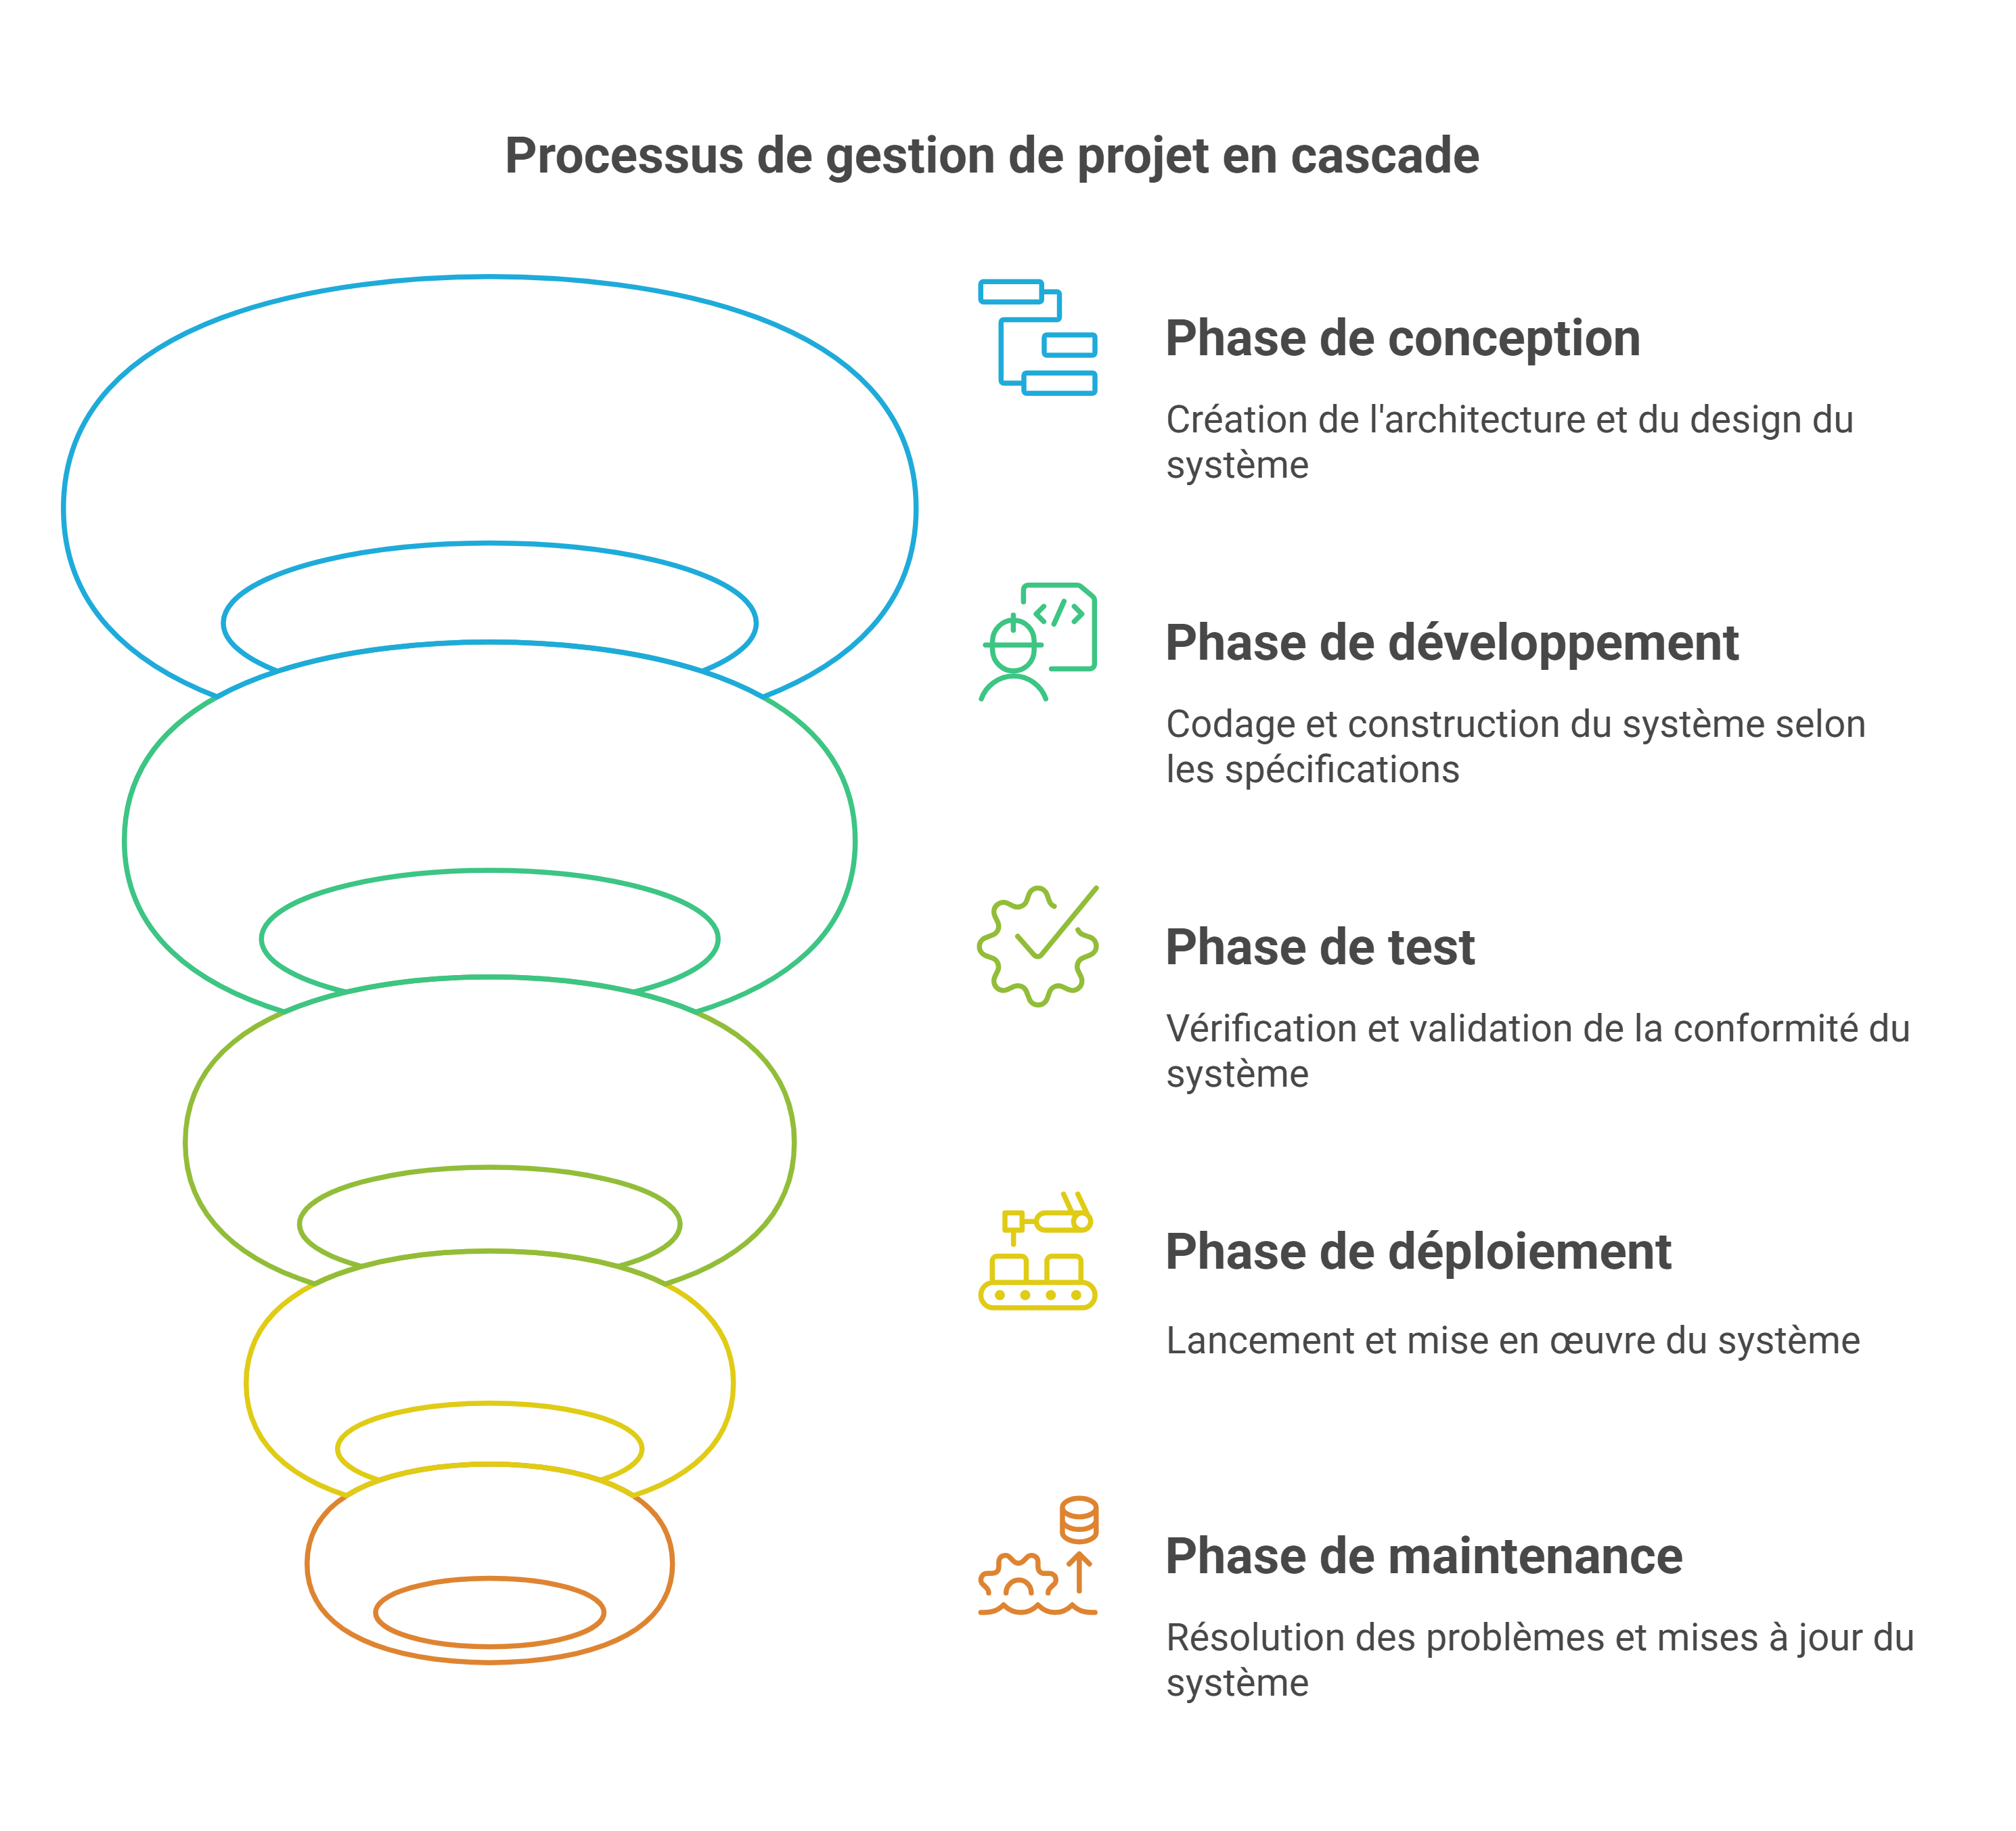
\includegraphics[width=15cm]{assets/presentation/waterfall.png}
\end{center}
\caption{Phases de la méthode Waterfall ou méthode en cascade}
\end{figure}

\subsection*{La méthode Agile}
La méthodologie Agile est un framework de gestion de projet qui divise les projets en plusieurs phases dynamiques appelées "Sprints". Contrairement aux méthodes traditionnelles qui requièrent une planification exhaustive du projet avant même le début du développement, la méthode Agile privilégie une approche itérative et incrémentale. Les objectifs sont fixés à court terme et le projet évolue au fur et à mesure que chaque sprint est réalisé. Chaque sprint vise ainsi à compléter une partie spécifique du projet, permettant d’ajuster continuellement les objectifs en fonction des retours du client et des évolutions du projet.

\vspace{0.3cm}

\begin{figure}[H]
\begin{center}
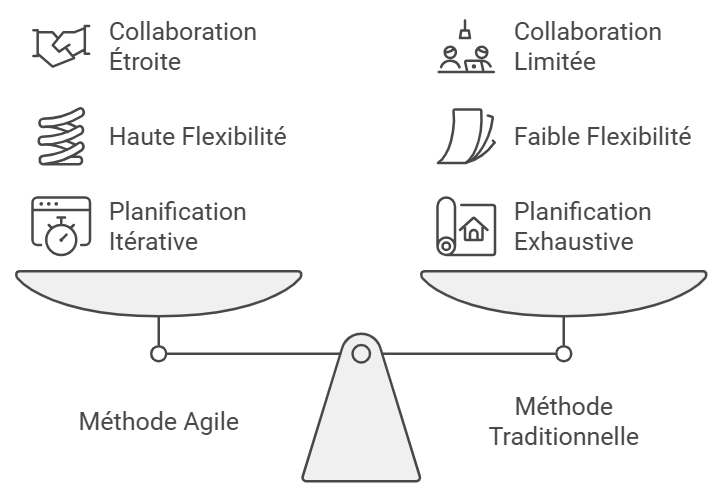
\includegraphics[width=15cm]{assets/presentation/1_gestion_agile_vs_gestion_traditionnelle.png}
\end{center}
\caption{Comparatif Gestion agile vs Gestion traditionnelle}
\end{figure}

La méthode Agile favorise une collaboration étroite entre les membres de l’équipe de développement, les utilisateurs et le client, renforçant ainsi la réactivité et l’efficacité du processus de développement. Cela se traduit par des échanges réguliers et des ajustements constants qui garantissent que le produit final répond précisément aux attentes et aux besoins des utilisateurs. Cette approche améliore non seulement la qualité du produit final, mais aussi la satisfaction du client, grâce à une flexibilité et une capacité d’adaptation accrues tout au long du projet. 

\vspace{0.3cm}

L'idée derrière ce framework de gestion de projets est de proposer rapidement une première version très minimaliste du produit (Minimum Viable Product MVP) qui répond au besoin des utilisateurs. Il réduit le délai entre la formulation d’un besoin et sa concrétisation. Le produit est enrichi au fur et à mesure et sa conformité est vérifiée régulièrement par l'équipe chargée des tests. Elle est souvent mise en œuvre à travers plusieurs variantes.

\vspace{0.35cm}
\begin{figure}[H]
\begin{center}
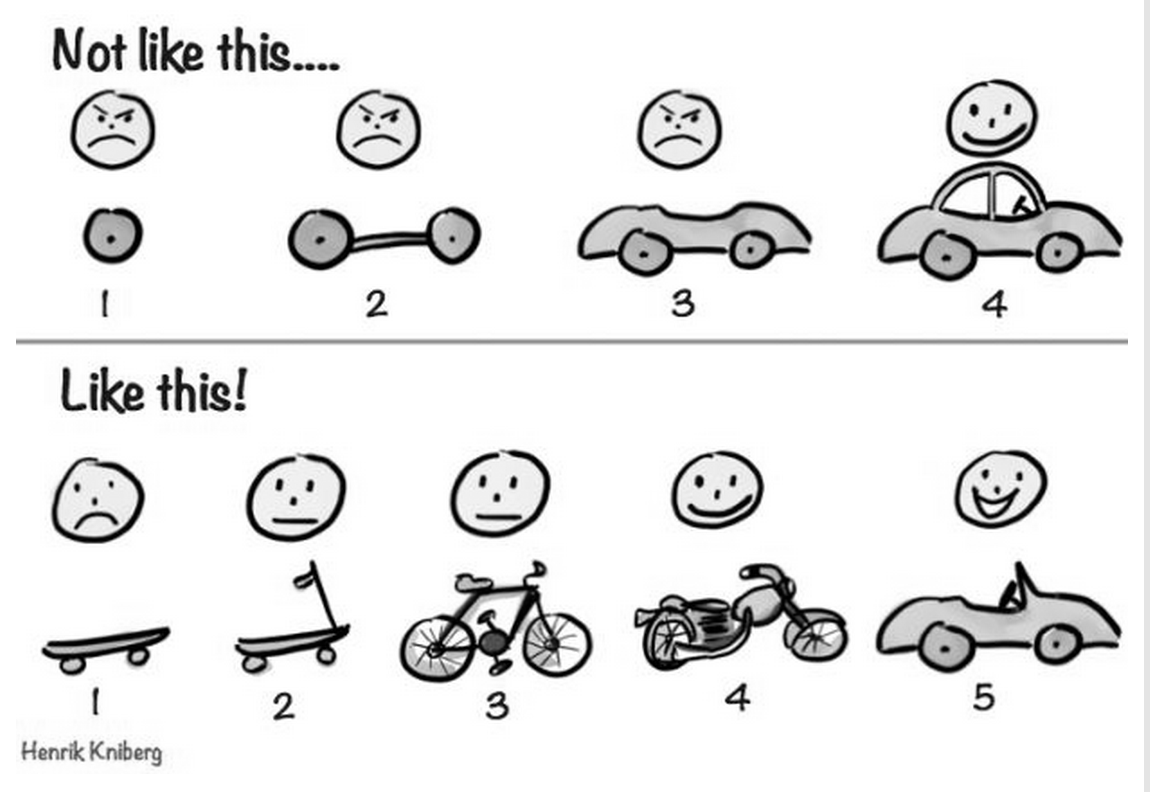
\includegraphics[width=15cm]{assets/presentation/3_mvp.png}
\end{center}
\caption{Exemple d'implémentation en Gestion agile vs Gestion traditionnelle}
\end{figure}

\vspace{0.35cm}

Selon le type de projets réalisés, de leur taille, des objectifs visés, ou même simplement la culture de l'entreprise, la méthode Agile peut être mise en œuvre sous plusieurs variantes. Parmi ces variantes, on retrouve notamment Scrum, Kanban et Extreme Programming (XP). Ces frameworks permettent tous d'adopter une approche itérative et incrémentale, mais se distinguent par leur manière d'organiser le travail.

\vspace{0.3cm}

La méthode Scrum est structurée autour de cycles de développement courts appelés sprints, avec des rôles spécifiques comme le Scrum Master et le Product Owner, et des cérémonies comme les réunions de planification, les revues et les rétrospectives. Extreme Programming (XP), de son côté, met l’accent sur les bonnes pratiques techniques comme le développement itératif et le test automatique pour améliorer la qualité du code et la réactivité aux besoins changeants des utilisateurs.

\vspace{0.3cm}

Chez JS Morlu, c'est la variante Kanban qui est privilégiée. Il s'agit d'un système visuel où les tâches sont réparties dans des colonnes représentant les différentes étapes du processus de développement, ce qui permet à l'équipe de suivre en temps réel l'avancement des travaux et d'identifier les goulots d'étranglement. L'absence de sprints prédéfinis permet une adaptation constante aux besoins du client et des priorités.

\subsection*{Communication au sein de l'entreprise} \label{comm_au_sein_de_l_entreprise}

Dans le cadre de ce projet, la collaboration s'est opérée essentiellement en ligne, compte tenu de la répartition géographique des équipes sur plusieurs pays. Nos équipes sont localisées au Sri Lanka, aux États-Unis (Virginie), en Malaisie, en Gambie et au Ghana. Cette diversité géographique représente un véritable défi organisationnel, mais elle est également une force, car elle permet de bénéficier de perspectives variées et d'une expertise diversifiée.

\vspace{0.35cm}

Pour assurer une communication fluide et efficace dans ce contexte international, un ensemble d'outils adaptés aux besoins de chaque situation est mis en place. 

\begin{itemize}
    \item \textbf{RingCentral} est utilisé pour les réunions formelles, notamment celles avec l'ensemble de l'équipe ou des réunions avec les clients, où il est important de partager des documents et des présentations en temps réel. Cet outil permet également de programmer des rencontres régulières pour suivre l'avancement des projets et clarifier les attentes des clients.

    \item \textbf{WhatsApp} pour les communications urgentes ou les échanges nécessitant une réponse immédiate, notamment lorsqu'une décision rapide doit être prise ou qu'un problème technique survient en dehors des heures de travail classiques.
\end{itemize}

\vspace{0.35cm}

Cette combinaison d'outils garantit une flexibilité optimale dans la gestion de nos interactions, tout en permettant de respecter les contraintes de décalage horaire entre les différents pays où se trouvent les membres de l'équipe.

\chapter{Présentation du projet}

\section{Contexte du Projet} \label{context_du_projet}

La création de \textbf{Fixaars}\footnote{Initialement \textbf{WowSoFast}} s’inscrit dans un contexte où la recherche de services professionnels au niveau local est encore fragmentée et peu accessible au Ghana. Bien que de nombreux particuliers et entreprises aient des besoins certes ponctuels mais variés en termes de services (plomberie, électricité, jardinage, etc.), ils sont souvent confrontés à une offre dispersée et à des difficultés pour trouver des prestataires qualifiés répondant à leurs critères spécifiques. Cette situation génère une perte de temps et une incertitude quant à la qualité des services disponibles.

\vspace{0.35cm}

Afin de répondre à cette problématique, le projet \textbf{Fixaars} a été initié avec pour objectif de créer une plateforme numérique innovante, capable de centraliser et de simplifier l’accès aux services locaux. Les besoins principaux exprimés par les utilisateurs ciblés au Ghana incluent la facilité d’utilisation, la transparence dans les informations sur les professionnels, et la possibilité de réserver des services adaptés à des critères variés (disponibilité, tarifs, proximité, avis).

\vspace{0.35cm}

L’application \textbf{Fixaars} répond également à un besoin d’adaptabilité et de personnalisation. Elle doit permettre aux utilisateurs de configurer leurs préférences en termes de types de services recherchés, de créneaux de disponibilité et de tarifs. De leur côté, les professionnels auront la possibilité de personnaliser leur profil pour mieux refléter leur expertise et de fixer leurs tarifs selon le marché.

\vspace{0.35cm}

L'ambition du projet est de répondre à la fois aux attentes des particuliers et aux exigences professionnelles des prestataires de services locaux. \textbf{Fixaars} se positionne ainsi comme un facilitateur qui souhaite offrir une expérience utilisateur fluide, pratique et de confiance, devenant une référence en matière de recherche de services locaux au Ghana.

\section{Utilisateurs Cibles}

Les utilisateurs cibles de l'application Fixaars sont divers et incluent :

\begin{enumerate}

    \item Individus à la recherche de services locaux : Qu'il s'agisse de n'importe quel service voulu, Fixaars serait le point de chutte parfait pour trouver le meilleur prestataire au meilleur prix.

    \item Prestataire de services locaux en quête de visiblité ou cherchant à aggrandire son portefeuille client; Entreprises offrant des services locaux précis ou variés 
    
\end{enumerate}

Ainsi, Fixaars vise à répondre aux besoins d'un large éventail d'utilisateurs, contribuant ainsi à simplifier et à améliorer la gestion des services locaux au Ghana, quel que soit le domaine d'activité ou la taille de l'organisation.

\section{Fonctionnalités Principales}

\begin{itemize}
    \item \textbf{Recherche de Services Locaux :} Les utilisateurs pourront effectuer des recherches ciblées pour trouver des professionnels locaux correspondant à leurs besoins spécifiques, que ce soit pour des services professionnels, personnels, éducatifs, ou autres.

    \item \textbf{Gestion des Profils Utilisateurs :} Les professionnels locaux auront la possibilité de créer des profils détaillés mettant en avant leurs compétences, expériences, tarifs, horaires de disponibilité, et recevront des évaluations de la part des utilisateurs.

    \item \textbf{Discussion instantannée et Appel Audio/Video intégré :} Les utilisateurs pourront discuter avec les professionnels locaux qu'ils recrutent par messagerie intégrée, optimisant ainsi l'accessibilté des services et la fluidité dans la prestation.

    \item \textbf{Système de Notation et d'Avis :} Les utilisateurs auront la possibilité de laisser des avis et des notations sur les professionnels, créant ainsi une communauté transparente où la qualité des services est mise en avant.

    \item \textbf{Configuration Personnalisée des Services :} Les utilisateurs pourront configurer leurs préférences en fonction de leurs besoins spécifiques, que ce soit en termes de services recherchés, de critères de sélection, ou de disponibilités.

    \item \textbf{Notifications Personnalisées :} Les utilisateurs recevront des notifications personnalisées sur les offres de services, les promotions, les disponibilités des professionnels, et d'autres informations pertinentes.

\end{itemize}

\vspace{0.5cm}

Ces fonctionnalités garantissent une expérience utilisateur complète et adaptée, simplifiant ainsi la recherche et la gestion de services locaux. Une présentation plus guidée de l'application est disponible dans l'annexe 1 de ce rapport.

\chapter{Analyse, Conception et Implémentation}

La modélisation joue un rôle clé dans le processus de développement d'un projet, car elle permet de structurer et de clarifier les besoins ainsi que la conception du système. Dans cette partie, nous présenterons l'exécution du projet, de l'analyse à l'implémentation. Nous allons décrire le modèle réalisé à l'issue de l'analyse du projet en expliquant les diagrammes fondamentaux conçus : le diagramme de cas d'utilisation et le diagramme de classes.

\vspace{0.35cm}

Le diagramme de cas d'utilisation a été utilisé en premier lieu pour identifier les fonctionnalités principales du système et les interactions entre les différents acteurs, qu'il s'agisse d'utilisateurs ou de systèmes externes. Il constitue une étape essentielle pour répondre à la question "Que doit faire le système ?".

\vspace{0.35cm}

Ensuite, le diagramme de classes a permis de définir la structure interne du système, en décrivant les objets nécessaires, leurs relations, ainsi que leurs attributs et méthodes. Basé sur les cas d'utilisation, ce diagramme répond à la question "Comment le système doit-il être conçu pour répondre aux besoins identifiés ?".

\vspace{0.35cm}

Afin d'assurer une réalisation optimale du projet en matière de durabilité et de pérennité du code, nous avons donc commencé à recueillir et modéliser les différentes informations disponibles. Dans ce contexte, nous avons choisi d'utiliser l'UML (Unified Modeling Language), un langage de modélisation unifié. Grâce à cette méthode, nous avons pu garantir une lecture homogène du modèle par toute l'équipe. Ceci a favorisé une meilleure compréhension du système par tous les membres de l'équipe. 

\vspace{0.35cm}

Pour élaborer notre modèle conformément à la norme UML, nous avons opté pour les programmes \textit{Modelio}\footnote{\url{https://www.modelio.org/}} et \textit{Draw.io}\footnote{\url{https://www.drawio.com/}}. Grâce à ces instruments fiables, nous avons pu représenter les informations, les interactions entre ces dernières, ainsi que les divers intervenants du système et les contextes d'utilisation qui leur sont assignés. Nous avons pu ainsi mettre en place les deux modèles, le diagramme de classes et le diagramme de cas d'utilisation. Le premier, orienté sur les données métiers et le second mettant en lumière les différents utilisateurs du système et les diverses actions que chacun d'eux peut déclencher sur le système.

\vspace{0.35cm}

Le fait que deux outils de modélisation assez complets (\textbf{Draw.io} et \textit{Modelio}) aient été mentionnés dans cette partie est justifiée. En effet, lors de la modélisation, nous avions initialement opté pour Modelio, dont j'étais déjà familier à la sortie de mon institut de formation. Cet outil permettait de réaliser la modélisation UML, la modélisation BPMN (Business Process Modeling Notation), SysML (Systems Modeling Language) ...

\vspace{0.35cm}

Par soucis de suivi des tâches, les diagrammes réalisés lors de la modélisation devraient être exportés au format SVG (\textit{Scalable Vector Graphics}) et ajoutés à l'outil de gestion de projet Jira. Les images au format SVG, contrairement aux images bitmap (PNG, JPEG, ...) peuvent être redimensionnées sans perdre en qualité. Ce format d'image offrait la possibilité de disposer des images de haute définition permettant donc de percevoir et visualiser les détails de l'image même quand on décide de zoomer au maximum dessus. Cette option d'exports d'images au format SVG n'était pas disponible avec Modélio. Et l'entreprise était déjà familière avec \textit{Draw.io}. C'est la raison pour laquelle Draw.io a été privilégié lors de cette étape de conception des diagrammes.

\section{Diagramme de Cas d'Utilisations}
Dans le cadre du projet Fixaars, le diagramme de cas d'utilisation a été essentiel pour clarifier les attentes des parties prenantes et structurer les fonctionnalités autour des besoins des utilisateurs.

\subsection{Acteurs identifiés}
Un acteur dans un système informatique représente une entité, humaine ou logicielle, qui interagit avec le système pour accomplir une tâche spécifique. Chaque acteur a des rôles et des responsabilités définis en fonction de ses interactions avec le système. 

\vspace{0.39cm}

Les principaux acteurs du système sont : 

\vspace{0.39cm}

\begin{itemize}
    \item \textbf{Le customer ou service seeker}: Il désigne l'utilisateur qui est à la recherche de professionnels locaux pour des services spécifiques sur la plateforme. 
    \item \textbf{Le service provider}: Il s'agit du prestataire de services locaux disponible sur la plateforme.
    \item \textbf{L'administrateur}: Ce dernier est responsable de la gestion et du monitoring du système.
\end{itemize}

\subsection{Cas d’Utilisation Clés}

Un cas d’utilisation décrit une interaction entre un acteur et le système afin d’atteindre un objectif spécifique. Il représente un scénario fonctionnel qui détaille comment un utilisateur ou un autre système interagit avec l’application pour réaliser une tâche précise.

\vspace{0.39cm}

Les cas d'utilisation identifiés pour chaque acteur incluent :

\vspace{0.39cm}

\begin{enumerate}
    \item \textbf{Le Customer} ou \textbf{Service Seeker} est l’utilisateur recherchant un service sur la plateforme. Il dispose des fonctionnalités suivantes : 
    \vspace{0.39cm}
        \begin{itemize}
            \item \textbf{Exploration des services} : Recherche de services en filtrant par localisation ou domaine de compétence. 
            \item \textbf{Consultation des profils professionnels} (profil, évaluations, disponibilité) : Ce cas d'utilisations permet à l'utilisateur d'accéder à toutes les informations relatives au professionnel qu'il  veut engager pour un service donné.
            \item \textbf{Renseigner les informations relatives au projet et engager le professionnel} : Possibilité d’envoyer une offre décrivant le projet et le budget alloué. Le prestataire peut accepter ou refuser la mission.
            \item \textbf{Contacter et discuter avec le professionnel sur la plateforme} : Contact direct via une messagerie instantanée intégrée. La plateforme autorise également l’accès aux numéros WhatsApp des prestataires pour des échanges externes.
            \item \textbf{Gerer ses projets} ( Consulter, Editer, Fermet le projet ou réassigner un nouveau professionnel au projet) : Ce cas d'utilisation offre à l'utilisateur un outil pour collaborer et suivre l'evolution de son projet avec le prestataire de service. Le prestataire de service a également une version de cet outil et peut interragir sur le projet également. Il peut mentionner s'il est d'accord pour travailler sur un projet, s'il a terminé ou s'il voudrait s'y retirer. Cette interface sert donc d'outil de travail collaboratif pour les deux utilisateurs
            \item \textbf{Ajouter un avis et une note au professionnel} : Attribution d’une note sur 5 et ajout d’un commentaire sur la qualité du service rendu, contribuant au classement des professionnels.
            \item \textbf{Accéder au chat} : Ceci permet d'accéder à l'ensemble des discussion en cours avec les prestataires de services.
            \item \textbf{Paramétrer son compte} : Permet la mise à jour des informations personnelles (nom, prénom, adresse, etc.) et des identifiants d’accès (email, numéro de téléphone, mot de passe).
        \end{itemize}

    \vspace{0.39cm}
    
    Le diagramme suivant illustre les différents cas d'utilisation propres au Service Seeker :

    \vspace{0.39cm}
        
    \begin{figure}[H]
    \begin{center}
    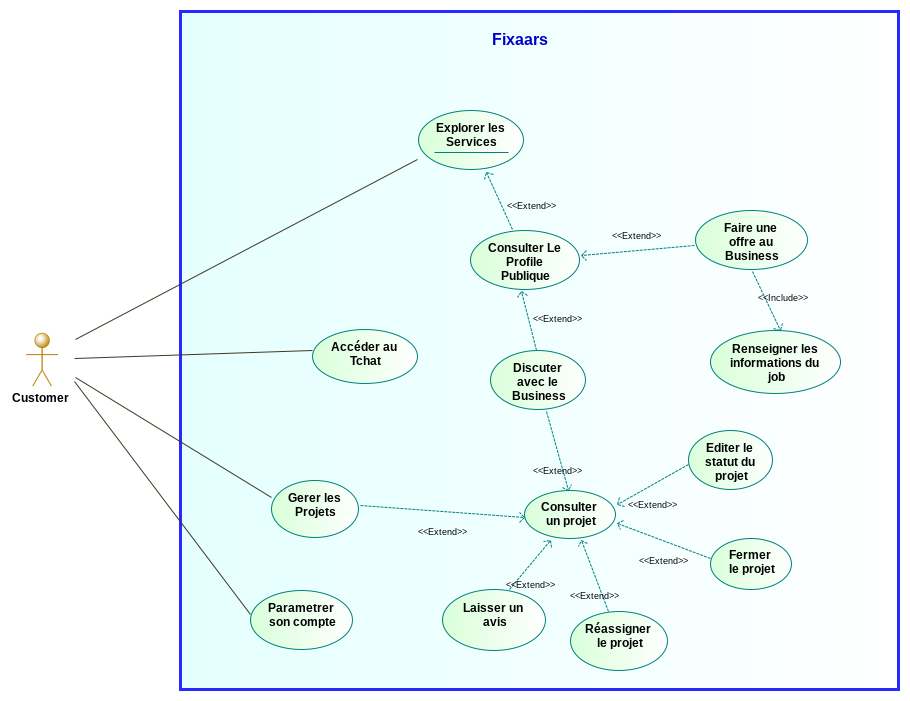
\includegraphics[width=17cm]{assets/diagrams/CustomerUC.png}
    \end{center}
    \caption{Modèle de cas d'utilisation du Customer}
    \end{figure}
    
    \vspace{0.39cm}

    L’analyse du diagramme de cas d’utilisation ci-dessus met en évidence différentes associations. On observe non seulement des liens entre l’acteur et les cas d’utilisation, mais aussi des relations entre certains cas d’utilisation eux-mêmes. Plus précisément, certaines associations utilisent le stéréotype « include », indiquant qu’un cas d’utilisation intègre systématiquement un autre dans son déroulement. D’autres associations sont de type « extend », ce qui signifie que le second cas d’utilisation est optionnel et ne se déclenche que sous certaines conditions.

    \vspace{0.39cm}

    Ainsi, selon le diagramme de cas d'utilisations ci-dessus, "Consulter le Profil Publique" est un cas d'utilisation optionnel qui vient enrichir le cas d'utilisation relatif à l'exploration des services. C'est à dire que lors de l'exploration des services, on peut (si on le désire,) consulter le profile Publique du prestataire. 

    \vspace{0.39cm}
    
    De la même manière, "Faire une offre au Business" est un cas d'utilisation qui intègre le cas d'utilisation "Renseigner les informations du job" dans son déroulement. En d'autre termes, pour faire une offre au business, il va falloir finir de renseigner les informations liées au Job.

    \vspace{1.39cm}
        
    \item \textbf{Le Business} ou \textbf{Le service provider} est l'utilisateur qui propose ses services sur la plateforme. En d'autres termes il s'agit du prestaire de service. Les fonctionnalités dont il dispose sont les suivantes :
    \vspace{0.39cm}
        \begin{itemize}
            \item \textbf{Exploration des jobs recommandés} : Le Business peut disposer des projets disponibles sur la plateforme et qui ne sont rattachés à aucun prestataire. Il s'agit nottament des offre déclinés par les prestataires initiaux des projets.
            \item \textbf{Discussion avec l'auteur du job} : Ce cas d'utilisation étend la fonctionalité d'exploration des jobs. Elle permet au prestataire de service d'entrer directement en contact avec l'utilisateur qui a posté le projet. 
            \item \textbf{Accéder au chat} : Tout comme l'utilisateur client (customer), le prestataire de service à aussi accès à l'ensemble des discussions en cours avec ses clients ou prospects.
            \item \textbf{Gestion de Projets} : Cette fonctionnalité est quelque peu limitées pour le Business. Elle lui permet tout comme au service seeker de suivre le projet. Mais les actions qu'il peut faire dessus sont : accepter ou décliner une offre, voir les avis et évaluations laissés par ses clients, voir les projets que les clients ont annulé ou fermé. 
            \item \textbf{Signaler un utilisateur de la plateforme} : Ceci permet de dénoncé un profil frauduleux à l'administrateur de la plateforme.
            \item \textbf{Parametrage de compte business} : Ce cas d'utilisation consiste en la mise à jour des informations relatives au profil et à l'activité professionnelle du prestataire de services. Il lui permet entre autre de mettre à jour la gamme de services qu'il supporte, sa disponibilité, sa localisation... Il peut également y configurer le coût moyen de chaque service offert.
        \end{itemize}
        
        \vspace{0.39cm}

        Le diagramme suivant illustre les différents cas d’utilisation
propres au Service Provider :

    \vspace{0.39cm}

    \begin{figure}[H]
    \begin{center}
    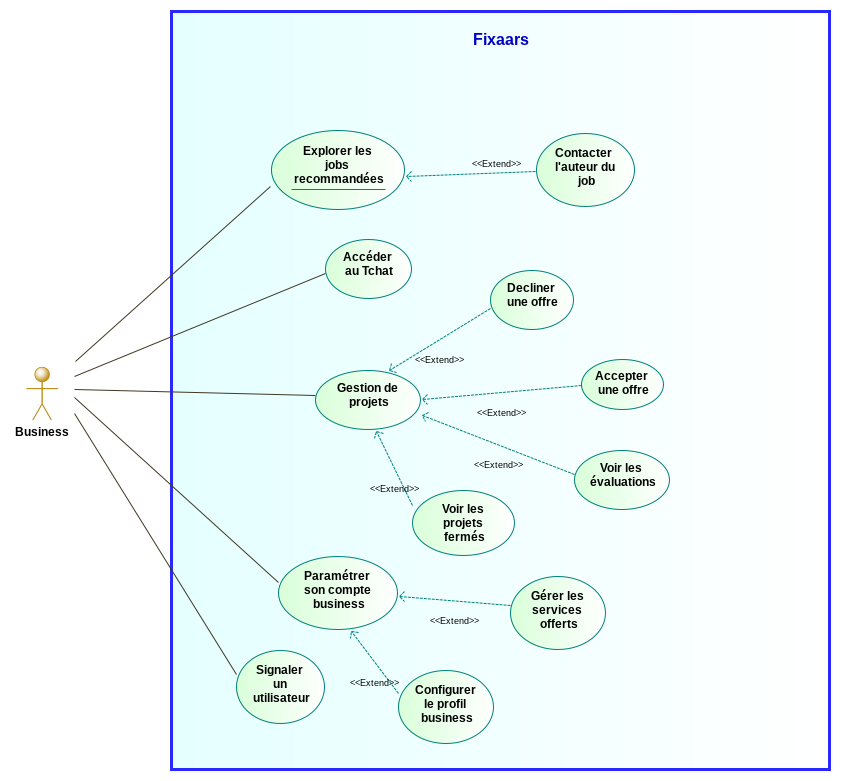
\includegraphics[width=17cm]{assets/diagrams/BusinessUC.png}
    \end{center}
    \caption{Modèle de cas d'utilisation du Business}
    \end{figure}
    
    \vspace{1.39cm}

    \item \textbf{L'administrateur} est le troisième acteur du système. Il est celui qui monitore le système. Les principaux cas d'utilisations qu'il implémente sont : 
        \begin{itemize}
            \item \textbf{Gestion des services et categories} : Ce cas d'utilisation comprend l'ajout, la suppression, la suspension momentannée, la mise à jour d'une catégorie de service ou d'un service. 
            \item \textbf{Gestion des utilisateurs} : Ceci permet de consulter la liste des utilisateurs de la plateforme, leur services proposés si ce sont des utilisateurs de type Business. 
            \item \textbf{Gérer les signalements} ou problèmes remontés par les utilisateurs : Ce cas d'utilisations permet de recueillir les différents signalements émis par les utilisateurs de la plateforme. Ceci permet à l'administrateur de prendre une décision appropriée.
        \end{itemize}
                
        \vspace{0.39cm}

        Le diagramme suivant illustre les différents cas d’utilisation
propres à l'administrateur du système :

    \vspace{0.39cm}

    \begin{figure}[H]
    \begin{center}
    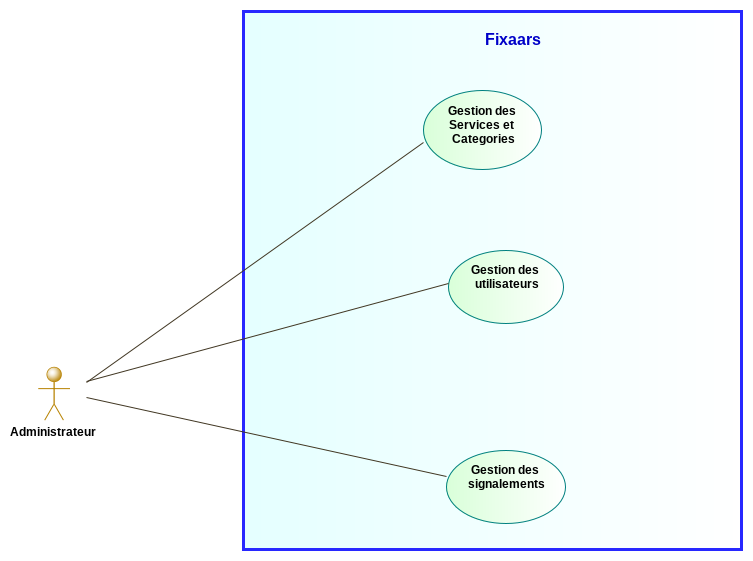
\includegraphics[width=17cm]{assets/diagrams/AdminUC.png}
    \end{center}
    \caption{Modèle de cas d'utilisation de l'Administrateur}
    \end{figure}
    
    \vspace{1.39cm}
\end{enumerate}

\vspace{0.5cm}

Les cas d'utilisation permettent d’identifier les principaux objets du système et leurs interactions. Le diagramme de classes en offre une représentation structurée en précisant leurs attributs, méthodes et relations. La section suivante présente ce diagramme, qui constitue la base de la conception technique du système.


\vspace{0.35cm}


\section{Diagramme de classes}
Le diagramme de classes est une représentation essentielle en conception orientée objet. Il définit les entités principales du système, leurs attributs, leurs méthodes et les relations qui les lient.
\\

Pour des soucis de présentation, j'ai organisé et structuré ce modèle sous forme de packages. En programmation orientée objet, un package est une unité logique de regroupement de classes. Il joue un rôle important dans :

\vspace{0.4cm}
\begin{itemize}
    \item La modularité : Chaque package est autonome et peut être modifié indépendamment.
    \item La lisibilité : Les classes sont catégorisées par domaine fonctionnel.
    \item La maintenabilité : L'isolation des responsabilités facilite l'identification des erreurs ou des améliorations.
\end{itemize}

\vspace{0.4cm}
Les packages permettent de regrouper des classes partageant des responsabilités ou des domaines fonctionnels similaires, favorisant ainsi une architecture modulaire et facile à maintenir. 

\vspace{0.4cm}

Dans la suite de cette partie, nous allons lister chaque package de notre modèle et les classes qui les composent. 

\subsection{Package User}
Ce package regroupe toutes les classes liées à la gestion des utilisateurs.
Il comprend les différentes classes suivantes :

\vspace{0.35cm}

\begin{itemize} 
    \item Classe \textbf{User} : Cette classe définit tous les attributs et méthodes inhérentes à un utilisateur. Elle  définit des attributs et méthodes dont hériterons beaucoup d'autres classes du même package.
    \item Classe \textbf{Role} : Cette classe représente le type d'utilisateur : Service provider, Service Seeker , Admin, ...
    \item Classe \textbf{Permission} : Représente le niveau d'autorisations de chaque rôle ou de chaque utilisateur dans le système. En d'autre termes, cette classe est responsable de ce que peut ou ne peut pas faire tel utilisateur ou tel rôle.
    \item Classe \textbf{Customer} : Elle implémente les attributs et méthodes inhérentes à un service seeker.
    \item Classe \textbf{Business} : Elle implémente les attributs et méthodes inhérentes à un service provider.

    \item \textbf{SocialAccountsBoard} : est une entité représentant un tableau d'informations sociales associé à un utilisateur de type Business sur la plateforme. Elle contient les URL des profils de médias sociaux que les utilisateurs peuvent enregistrer pour promouvoir leurs services ou établir une présence en ligne. 

    \vspace{0.35cm}

    Lorsqu'un service seeker consulte un profil d'un service provider sur la plateforme, les liens vers les réseaux sociaux stockés dans cette entité peuvent être affichés, offrant un accès rapide aux profils sociaux pour une meilleure évaluation de l'entreprise.
\end{itemize}

\vspace{0.35cm}

\begin{figure}[H]
\begin{center}
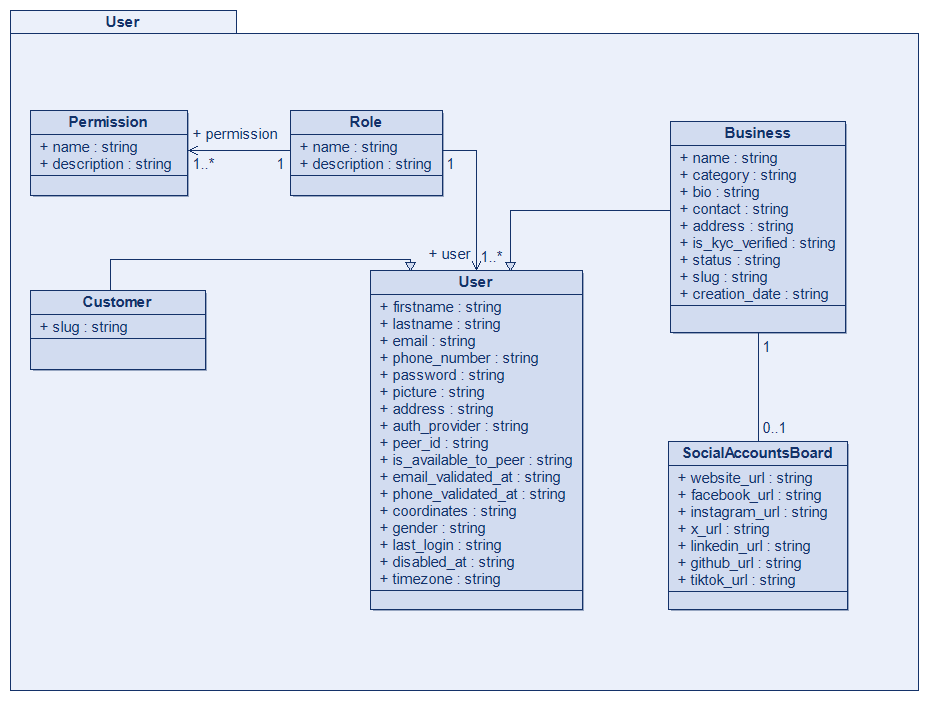
\includegraphics[width=15cm]{assets/diagrams/UserPackage.png}
\end{center}
\caption{Modèle Relationnel du Package User}
\end{figure}
\vspace{0.35cm}

\newpage

\subsection{Package Catalog}
Le package Catalog comprend toutes les entités qui enrichissent et structurent les données contextuelles essentielles à l'utilisation de la plateforme. Ces entités sont principalement liées à la gestion des informations géographiques, à la gestion des devises, ainsi qu'à la section FAQ ( Frequently Asked Questions) pour les prestataires de services. 

\begin{itemize}
    \item Classes liées à la géolocalisation des prestataires de services : Ces classes permettent de décrire les informations géographiques des prestataires de services. Elles aident à associer chaque prestataire à un emplacement spécifique pour que les utilisateurs puissent facilement rechercher des services en fonction de leur emplacement.
    Elles incluent les entités \textbf{Area , Town, Constituency, District, Country, Region}
    \item Classe \textbf{FAQ} : Cette classe permet aux prestataires de services de définir des questions fréquemment posées (FAQ) et de fournir des réponses aux utilisateurs, afin de clarifier les informations sur leurs services sans besoin de contact direct.
    \item Classe \textbf{Currency} Cette classe représente les différentes monnaies utilisées sur la plateforme, permettant la gestion des devises et la conversion des prix selon la localisation des utilisateurs.

    \item Classe \textbf{ProfileView} : Représente la vue du profil d'un utilisateur sur la plateforme. Cette classe est utilisée pour afficher les informations pertinentes sur les vues de profil d'un service provider par un service seeker. C'est une classe de logging (journalisation) essentielle dans la stratégie commerciale liée au projet.

    \item Classe \textbf{Service} : Représente les services supportés par la plateforme. Cette classe est utilisée pour enrichir les compétences des prestataires de services sur la plateforme. 

    \item Classe \textbf{Service Category} : Représente la catégorie à laquelle appartient un ou plusieurs services offerts sur la plateforme. Cette classe permet de grouper les services pour une meilleure organisation.

    \item Classe \textbf{ServiceProvided} : Cette classe sert de classe association dans la relation qui lie la classe Service et la classe Business. Elle sert à décrire les services supportés par chaque Business. On peut dénoter une association de type \textbf{many-to-many} qui relie la table Service à la table Business. 
    
    \textbf{Une classe association} est une classe qui sert d’intermédiaire dans une relation many-to-many entre deux entités, tout en stockant des informations propres à cette relation.
    
    \item Classe \textbf{Assignment} : Cette classe sert de classe association entre les utilisateurs et le projet. En effet, à chaque projet créé, plusieurs utilisateurs peuvent être associés, notamment le créateur du projet et le prestataire de services. Aussi, à chaque utilisateur, on peut très bien associé plusieurs projets gérées. Ceci traduit une relation de type \textbf{many-to-many}. 

\end{itemize}

    \vspace{0.35cm}

Chaque classe de ce package a un rôle précis dans l'enrichissement des données et dans l'amélioration de l'expérience utilisateur, qu'il s'agisse de la recherche géographique, de la gestion des devises, ou de l'assistance via les FAQ. 

    \vspace{0.35cm}

\begin{figure}[H]
\begin{center}
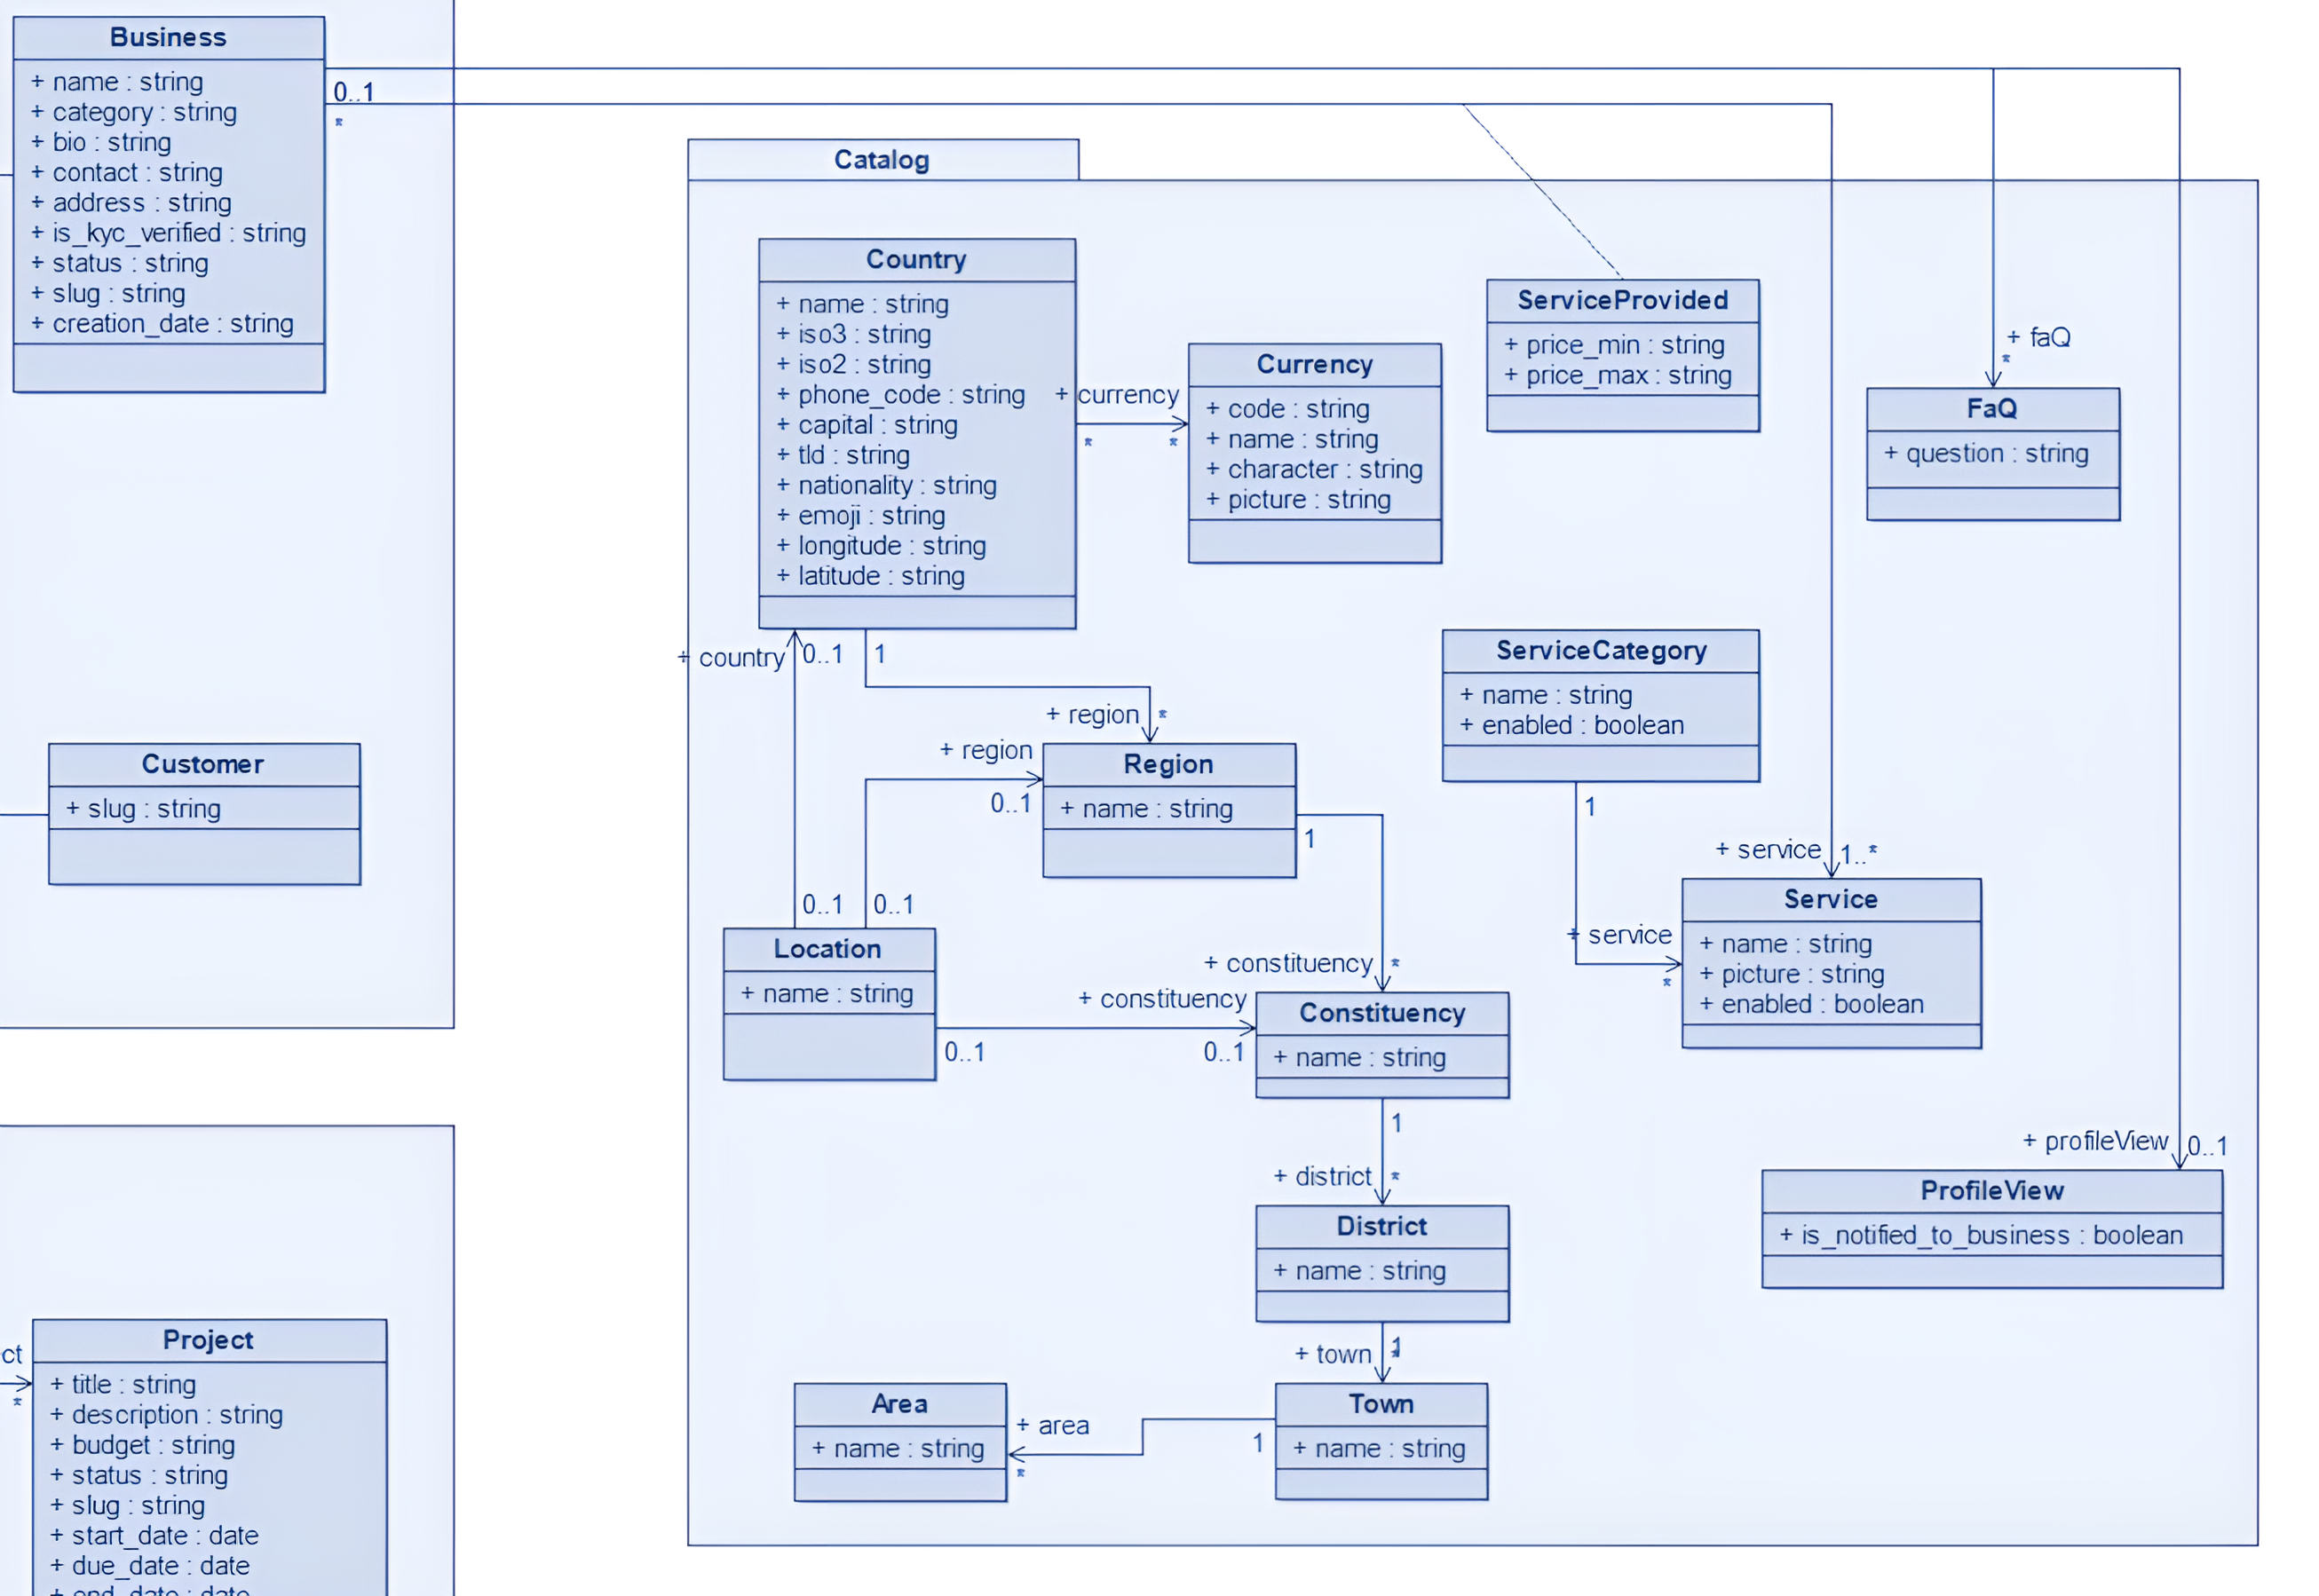
\includegraphics[width=15cm]{assets/diagrams/CatalogUC1.png}
\end{center}
\caption{Modèle Relationnel du Package Catalog}
\end{figure}
\vspace{0.35cm}

Comme le montre le diagramme ci-dessus, toutes les classes liées à la localisation géographique sont liées entre elles. Ainsi, on peut facilement associer une ville ou une région quelconque à un business et déterminer les subdivisions couvertes par cette ville ou région (district, quartier, ...) et ses subdivisions parentes (pays, ... ).

\vspace{0.35cm}

La classe Service est en relation avec la classe ServiceCategorie. Le type d'association qui lie les deux classes est du \textbf{one-To-many} et \textbf{many-To-one}. En effet, cette association traduit le fait qu'à un service (Service) on n'associe qu'une seule et unique catégorie de service (ServiceCategory). Inversement, à chaque catégorie de service (ServiceCategory), on peut associer plusieurs services (Service). 

\subsection{Package Communication} \label{subsection_package_communication}
Ce package concerne toutes les fonctionnalités liées à la communication instantanée (chat) entre les utilisateurs du système. Ce package regroupe les classes et les modèles qui gèrent les échanges de messages (textuels et vocaux), les appels (audio et vidéo), ainsi que les discussions privées. Voici une explication détaillée du contenu.

\begin{itemize}
    \item Classe \textbf{Attachment} : Représente les pièces jointes envoyées dans les conversations, qu'il s'agisse de fichiers, images, vidéos, ou tout autre type de média. Elle contient des informations telles que le type de fichier, la taille, le nom et le lien vers le fichier.

    \item Classe \textbf{Room} : Ce modèle représente une salle de discussion. Il contient des informations sur les participants, le nom de la salle (si applicable), l'historique des messages, et des métadonnées sur la salle (si elle est privée, publique, ou verrouillée, par exemple).

    \item Classe \textbf{Message} : Ce modèle gère les messages textuels envoyés dans les conversations. Il contient des informations sur le contenu du message, l'utilisateur qui l'a envoyé, la date et l'heure d'envoi, ainsi que des références à d'éventuelles pièces jointes ou appels associés.

    \item Classe \textbf{Call} : Représente un appel, qu'il soit audio ou vidéo, entre deux utilisateurs. Il contient des informations sur l'état de l'appel (en cours, terminé, rejeté), les participants, le type d'appel (audio ou vidéo), et des métadonnées comme la durée de l'appel.
\end{itemize}

\vspace{0.35cm}

Ce package représente un aspect essentiel de la plateforme, car il permet de gérer les interactions en temps réel entre les utilisateurs. En regroupant des éléments tels que les messages textuels/audio, les appels audio/vidéo, et les pièces jointes, ce package est conçu pour offrir une structure modulaire et cohérente, facile à maintenir et à étendre à l'avenir.

\begin{figure}[H]
\begin{center}
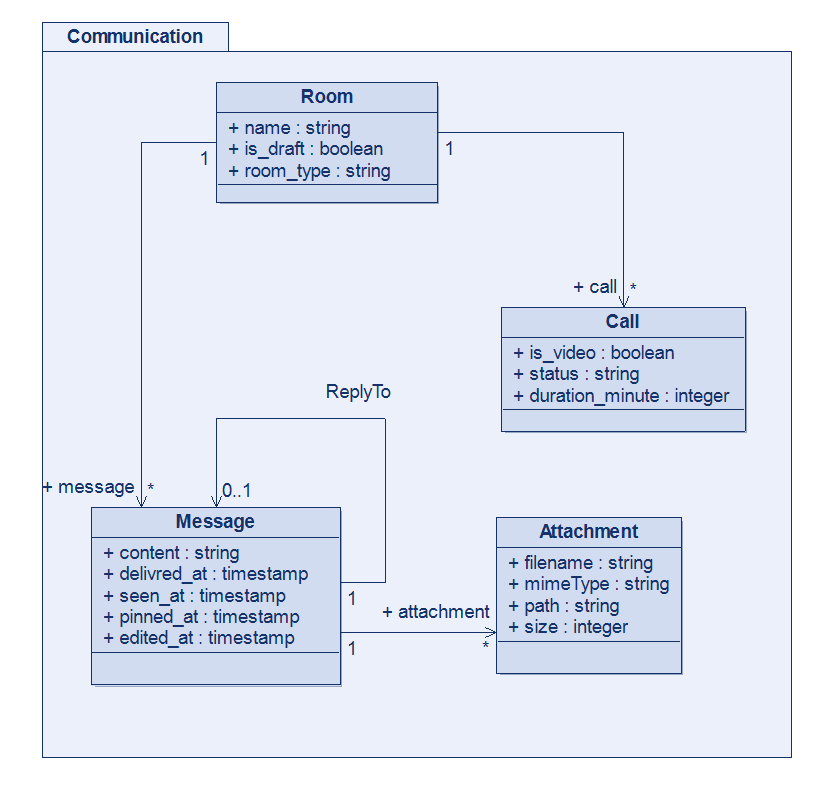
\includegraphics[width=15cm]{assets/diagrams/CommunicationPackage.png}
\end{center}
\caption{Modèle Relationnel du Package Communication}
\end{figure}
\vspace{0.35cm}

\subsection{Package Project}
Ce package regroupe toutes les classes et modèles qui aident à gérer les projets sur la plateforme, en particulier ceux liés aux réservations et aux affectations de services. Ces classes sont utilisées pour suivre les détails du projet, les avis, la localisation, ainsi que pour l'archivage. Lorsqu'un service seeker réserve un service, ces modèles enrichissent les données du projet en cours, en stockant des informations clés, comme l'assignation des prestataires, la localisation, et les évaluations des services rendus.

\vspace{0.35cm}

\begin{itemize}

    \item Classe \textbf{Project} :  Ce modèle représente le projet ou job crée par le service seeker. Il contient des informations sur le type de service réservé, l'utilisateur qui l'a réservé, le prestataire assigné, le statut du projet (en cours, terminé, annulé), les dates de début et de fin, et d'autres informations spécifiques au projet.

    \item Classe \textbf{Assignment} : Cette classe sert de classe association entre les utilisateurs et le projet. En effet, à chaque projet créé, plusieurs utilisateurs peuvent être associés, notamment le créateur du projet et le prestataire de services. Aussi, à chaque utilisateur, on peut très bien associer plusieurs projets gérés. Ceci traduit une relation de type \textbf{many-to-many}. 

    \item Classe \textbf{Review} :  Ce modèle représente les évaluations laissées par les utilisateurs (service seekers) sur les services fournis par les prestataires lorsque le projet est terminé ou annulé. Il contient des informations sur la note attribuée, les commentaires et la date de l'évaluation. Ces évaluations sont destinées à être affichées publiquement sur le profil du prestataire de service dans l'application.

    \item Classe \textbf{Report} : Cette classe représente les signalements emis par un service provider sur un profil de service seeker ou vice versa. Ces signalements sont destinés à être envoyés à l'administrateur pour une prise de mesures adéquate sur le profil signalé. 

    \item Classe \textbf{ReportInfo} : C'est une classe association qui lie chaque objet "Report" à plusieurs objets "Users" et vice versa. En effet, un utilisateur peut émettre un signalement contre un autre utilisateur. Cela nous rammène toujours à la relation \textbf{many-to-many} dont nous avons fait cas tantôt au niveau de la classe \textbf{Assignment}
\end{itemize}

\vspace{0.35cm}

\begin{figure}[H]
\begin{center}
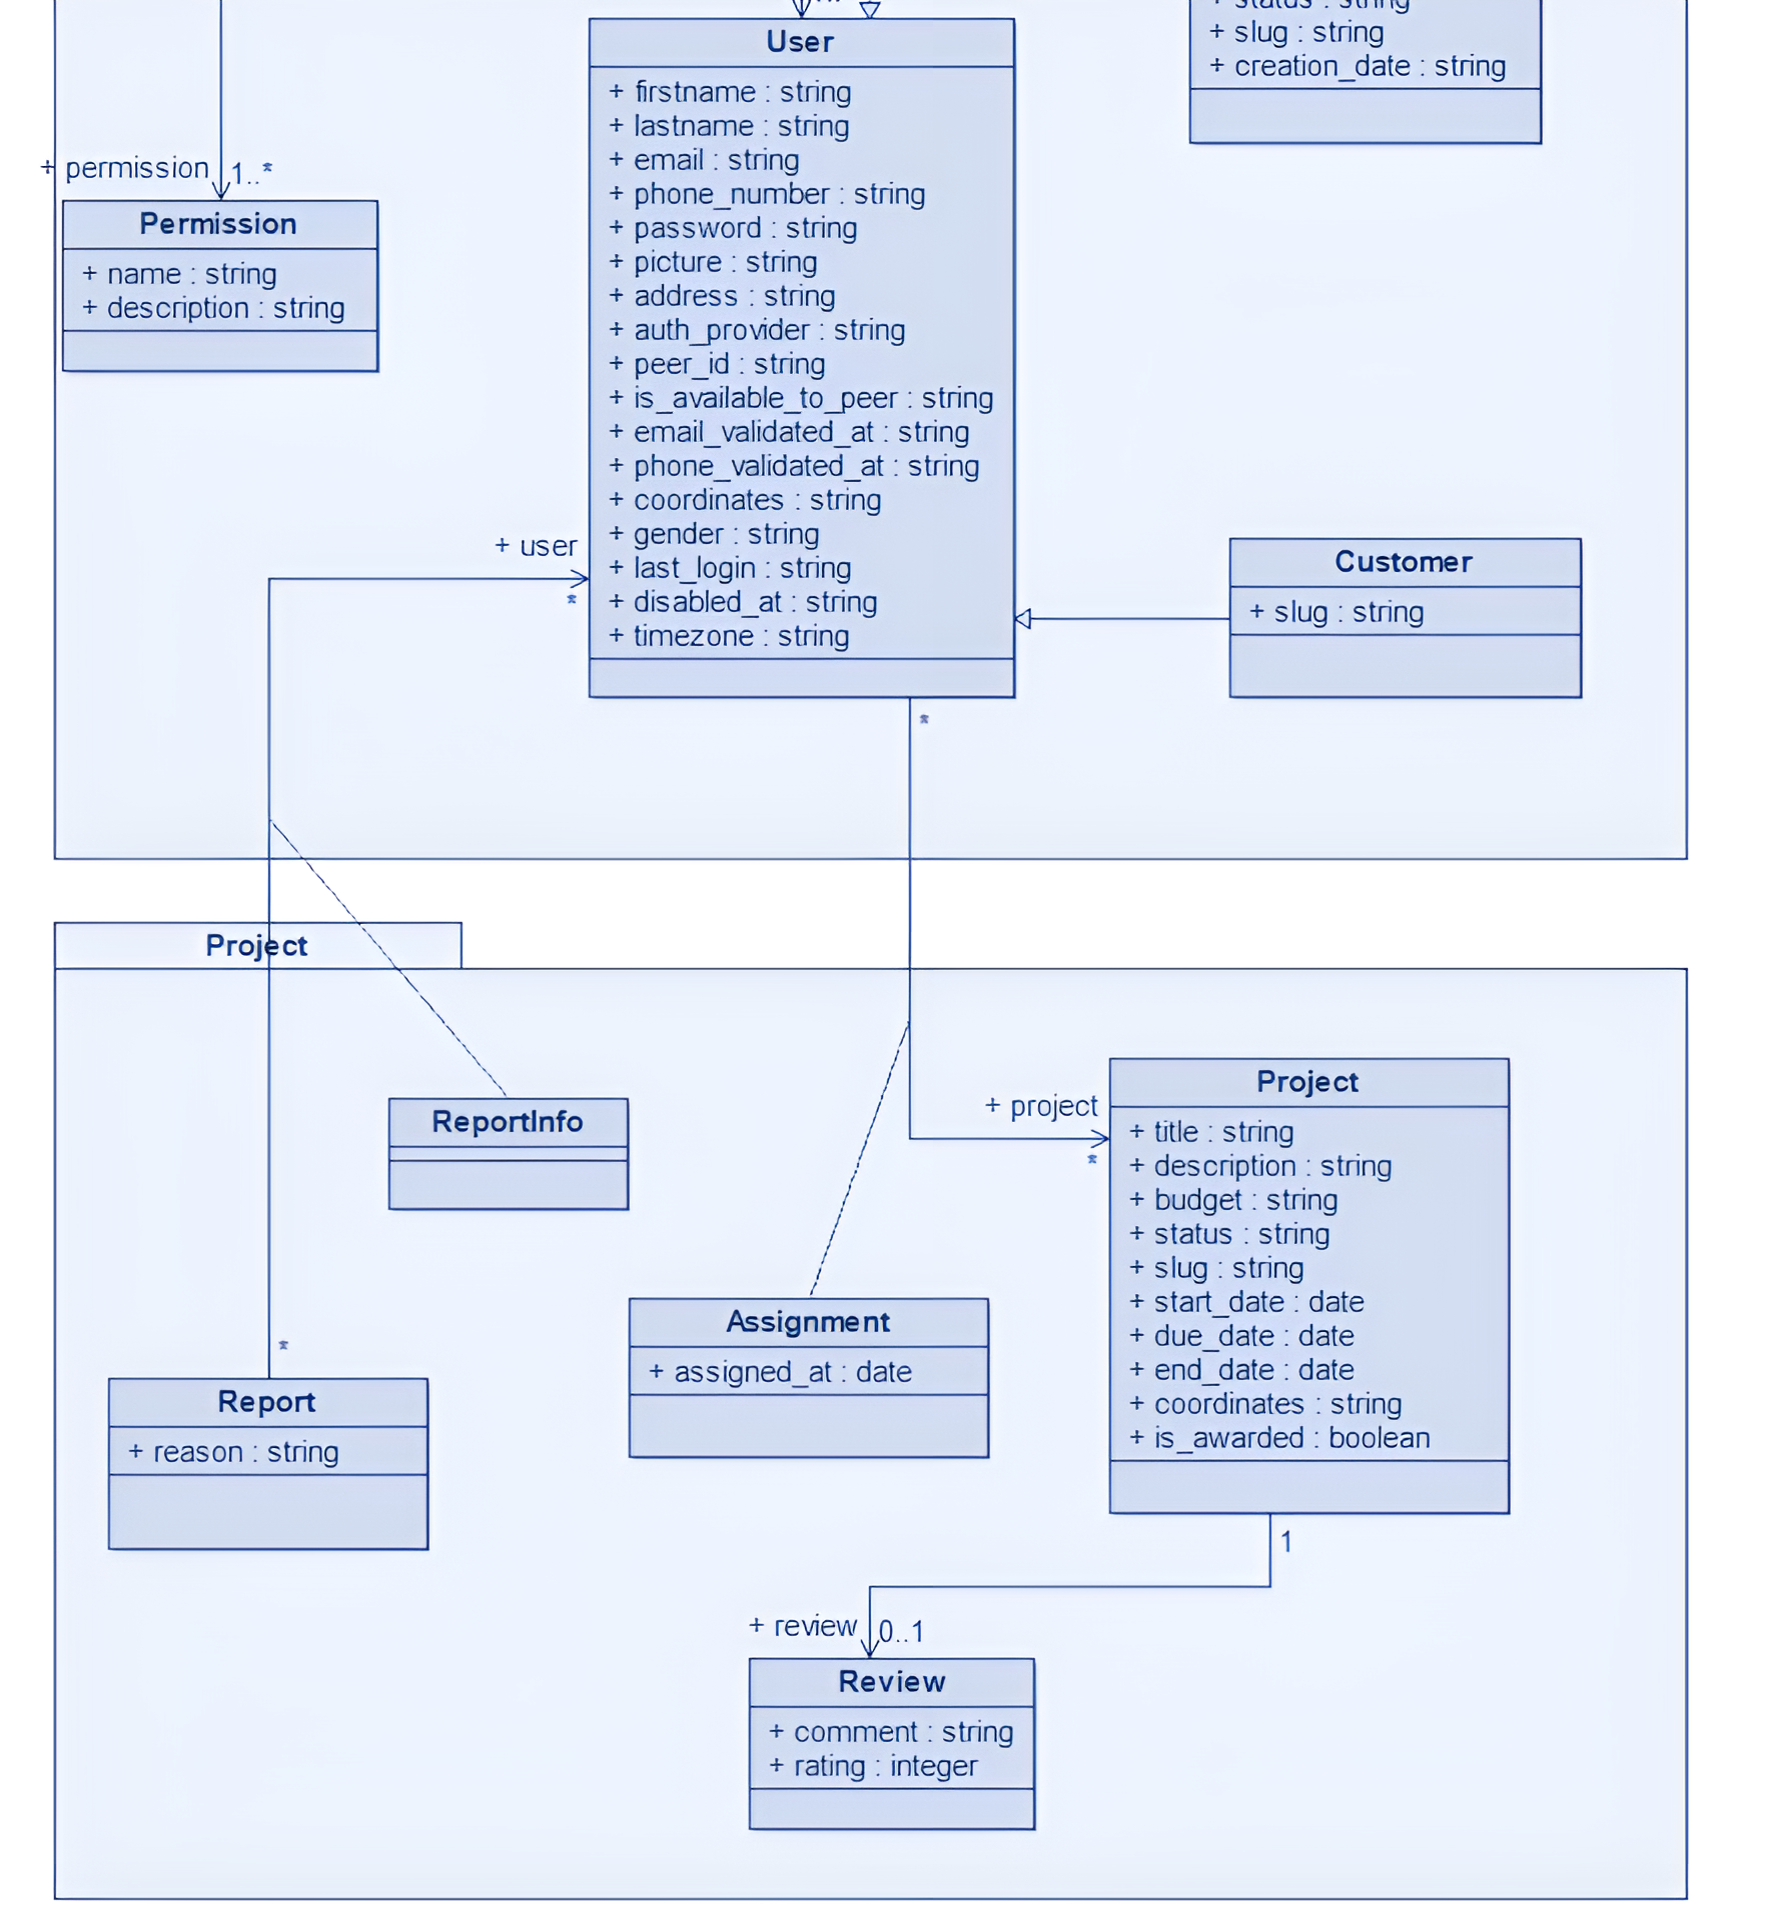
\includegraphics[width=15cm]{assets/diagrams/ProjectUC.png}
\end{center}
\caption{Modèle Relationnel du Package Project}
\end{figure}

\vspace{0.35cm}

\newpage

\section{Stack Technologique}
Le développement de la solution repose sur une stack technologique choisie pour ses avantages en termes de performance, de flexibilité et de maintenabilité. La plateforme est principalement construite en Node.js avec TypeScript et utilise une architecture modulaire pour organiser les différents composants logiciels. Cette approche a permis de garantir une gestion fluide du code, une facilité d'évolution et une séparation claire des responsabilités. Cette partie détaille les technologies et les choix d'architecture utilisés pour développer cette solution.

\subsection*{Technologies utilisées}
\subsubsection*{Node.js}
Node.js est un environnement d'exécution pour le JavaScript côté serveur. Il permet d'exécuter du JavaScript en dehors du navigateur, ce qui est particulièrement utile pour construire des applications web côté serveur. Node.js est conçu pour être non-bloquant, léger et efficace pour les applications qui nécessitent une gestion des connexions simultanées et une architecture extensible. C'est cette performance que nous avons exploitée pour assurer la réactivité et l'évolutivité de notre application.

\begin{figure}[H]
\begin{center}

\includegraphics[width=10cm]{assets/presentation/Node_logo_NodeJS-700x428.png}
\end{center}
\caption{Logo Node.js}
\end{figure}

\subsubsection*{Express.js}
Express.js est une librairie Node.js qui simplifie la création d'applications web et d'APIs. Avec Express, la gestion des requêtes HTTP, la configuration des routes et la gestion des middlewares deviennent beaucoup plus simples. Express fournit également un environnement flexible qui permet d'utiliser des moteurs de template comme EJS pour générer des pages HTML dynamiques côté serveur.\\\\

\begin{figure}[H]
\begin{center}

\includegraphics[width=10cm]{assets/presentation/express.js_Logo-700x156.png}
\end{center}
\caption{Logo Express.js}
\end{figure}

\subsubsection*{TypeScript}
TypeScript est un sur-ensemble de JavaScript qui ajoute un système de typage statique au langage. Son utilisation dans ce projet permet de réduire les erreurs courantes liées à la gestion de types dynamiques dans JavaScript. En fournissant une validation de types à la compilation, TypeScript améliore la sécurité du code, facilite le refactoring et rend le projet plus maintenable à long terme. Cette approche statique est particulièrement bénéfique dans les projets de grande envergure, comme celui-ci, car elle aide à mieux organiser le code et à éviter des erreurs complexes lors du développement.\\\\

\begin{figure}[H]
\begin{center}

\includegraphics[width=15.5cm]{assets/presentation/TypeScript.jpg}
\end{center}
\caption{Logo TypeScript}
\end{figure}

\subsubsection*{TypeORM}
TypeORM est un ORM (Object-Relational Mapping) pour Node.js et TypeScript. Il permet de travailler avec une base de données relationnelle comme PostgreSQL en utilisant des objets JavaScript/TypeScript plutôt que d'écrire directement des requêtes SQL. TypeORM facilite la gestion de la base de données en automatisant de nombreuses tâches telles que les migrations, la gestion des entités et des relations entre celles-ci. Grâce à TypeORM, nous avons pu définir des modèles d'entités qui mappent directement les tables de la base de données PostgreSQL, simplifiant ainsi l'interaction avec la base de données.\\\\

\begin{figure}[H]
\begin{center}

\includegraphics[width=5cm]{assets/presentation/TypeORM.png}
\end{center}
\caption{Logo TypeORM}
\end{figure}

\subsubsection*{PostgreSQL}
PostgreSQL est une base de données relationnelle open source puissante, utilisée pour stocker les données du projet. Sa robustesse, sa capacité à gérer de grandes quantités de données et son support des transactions complexes en font un excellent choix pour les applications d'envergure. Nous avons choisi PostgreSQL pour sa stabilité et son large écosystème de bibliothèques et d'outils compatibles.\\\\\\\\

\begin{figure}[H]
\begin{center}

\includegraphics[width=13cm]{assets/presentation/PostgreSQL_logo_Postgre_SQL-700x108.png}
\end{center}
\caption{Logo PostgreSQL}
\end{figure}


\subsubsection*{EJS et Bootstrap}
EJS (Embedded JavaScript) est un moteur de template utilisé pour générer des pages HTML dynamiques côté serveur. Il nous a permis de créer des vues interactives qui se mettent à jour en fonction des données côté backend. 

\begin{figure}[H]
\begin{center}

\includegraphics[width=15cm]{assets/presentation/ejs.png}
\end{center}
\caption{Logo EJS}
\end{figure}

D'autre part, Bootstrap a été utilisé pour la mise en page et le style de l'interface utilisateur, offrant ainsi une base solide pour la conception de pages web réactives.\\\\

\begin{figure}[H]
\begin{center}

\includegraphics[width=5cm]{assets/presentation/Bootstrap_Logo-700x700.png}
\end{center}
\caption{Logo Bootstrap}
\end{figure}

\subsubsection*{PeerJS et Socket.io}  
Pour la gestion de la communication en temps réel dans notre projet, nous avons utilisé \verb|PeerJS| et \verb|Socket.io|.  

\verb|PeerJS| est une bibliothèque JavaScript qui facilite l'utilisation de WebRTC pour établir des connexions pair-à-pair. Elle nous a permis d'implémenter une fonctionnalité d'appel vidéo instantané en simplifiant la gestion des flux audio et vidéo. Grâce à PeerJS, les utilisateurs peuvent initier et recevoir des appels en toute transparence sans nécessiter de configuration complexe côté client.  

\vspace{0.35cm}

\begin{figure}[H]
\begin{center}

\includegraphics[width=7cm]{assets/presentation/peer-js.jpeg}
\end{center}
\caption{Logo PeerJS}
\end{figure}

\verb|Socket.io|, quant à lui, a été utilisé pour la gestion des communications en temps réel basées sur les sockets. Il permet d'établir une connexion bidirectionnelle entre le serveur et les clients, facilitant ainsi les échanges instantanés de messages et d'événements. Cette technologie a été essentielle pour la mise en place du chat en direct et de la signalisation WebRTC nécessaire aux connexions PeerJS.  

\vspace{0.35cm}

\begin{figure}[H]
\begin{center}

\includegraphics[width=7cm]{assets/presentation/socketio.png}
\end{center}
\caption{Logo Socket.io}
\end{figure}

L'intégration de PeerJS et Socket.io a permis d'assurer une communication fluide et réactive entre les utilisateurs, offrant ainsi une expérience utilisateur optimale pour le chat et les appels vidéo en direct.  

\subsubsection*{Git, Bitbucket et CI/CD}
Le versionnement du code du projet est géré avec Git et hébergé sur Bitbucket, une plateforme de gestion de code source qui permet de travailler de manière collaborative. Pour assurer la qualité du code et l'intégration continue, un pipeline CI/CD (Continuous Integration / Continuous Deployment) a été mis en place. Celui-ci est connecté à un serveur VPS sur Hostinger, permettant d’automatiser les tests, le déploiement et la mise à jour de l’application à chaque changement de code.

\subsubsection*{Jira}
Jira a été utilisé pour la gestion de projet, permettant de suivre l'avancement des tâches, de planifier les sprints et d'assigner les responsabilités à chaque membre de l'équipe. Cette plateforme a facilité la collaboration et la coordination au sein de l'équipe de développement.\\\\

\begin{figure}[H]
\begin{center}

\includegraphics[width=15cm]{assets/presentation/JIRA.jpeg}
\end{center}
\caption{Logo Jira}
\end{figure}


\subsection*{Approche de développement}
\subsubsection*{Backend-first Development}
Dans une approche Backend-first, nous avons commencé par concevoir et développer l'API avant d'implémenter le frontend. Cela a permis de nous concentrer sur les besoins en données et sur la structure de l'API sans être influencés par des contraintes frontend. Cette approche garantit que le backend est indépendant du frontend, ce qui permet de créer un frontend qui peut s'adapter à n'importe quelle structure de données définie par l'API.

\subsubsection*{API-first Design}
Le API-first design a guidé la conception de notre projet. Les APIs ont été définies dès le début, avec des spécifications claires des endpoints, des méthodes HTTP, des formats de réponse et des erreurs possibles. Nous avons documenté ces APIs dans une collection Postman, ce qui nous a permis de tester chaque endpoint, de fournir des exemples de réponses et d’assurer une intégration fluide avec le frontend.

\subsection*{Tests et Documentation}
\subsubsection*{Postman}
Postman a été utilisé pour la documentation, les tests et l’automatisation des requêtes API. La collection Postman contient tous les endpoints de l'API avec des exemples de requêtes et de réponses. Nous avons également configuré des environnements pour tester l’API dans différents contextes (par exemple, en développement, en production, etc.). Les scripts d’automatisation ont été utilisés pour exécuter des tests de manière continue et vérifier la validité des endpoints. \\\\

\begin{figure}[H]
\begin{center}

\includegraphics[width=15cm]{assets/presentation/postman-logo-vert-2018.jpg}
\end{center}
\caption{Logo Postman}
\end{figure}


\subsubsection*{Versioning et CI/CD}
Le code est versionné via Git et hébergé sur Bitbucket. À chaque modification de code, les tests sont automatiquement exécutés dans le pipeline CI/CD configuré sur un serveur VPS de Hostinger. Cette démarche permet de garantir que chaque modification n'introduit pas de régressions et que le code est toujours dans un état déployable.

\subsection*{Vues}
Le frontend utilise Express.js pour le routage des pages, EJS pour la génération des vues dynamiques côté serveur, et Bootstrap pour la mise en page. Cette approche est complémentaire à l'architecture backend-first et permet une gestion fluide de l'interface utilisateur en fonction des données fournies par le backend.

\section{Développement de la solution} \label{developement_solution}

Après avoir réalisé l’analyse, la conception et le choix des technologies, la phase suivante du projet était le développement. Cette étape consistait en l’implémentation des fonctionnalités définies en respectant la stack technologique choisie et les contraintes techniques imposées.

\vspace{0.35cm}

Tout le long de cette partie, nous allons expliquer étape par étape comment le projet a été construit. Nous  aurons une vision axée sur la partie backend du projet, puis ensuite nous parlerons de la partie frontend.

\subsection*{Présentation technique du backend} \label{architecture_backend}

Étant donné que nous travaillions avec \textbf{Node.js} et \textbf{TypeScript}, nous avons suivi les pratiques basiques pour structurer notre projet de manière modulaire et maintenable. L’initialisation s’est faite en plusieurs étapes :

\begin{enumerate}
    \item \textbf{Création du projet} : 
    
    Dans un dossier raçine du projet, nous avons initialisé le projet npm via la commande suivante : 

    \begin{verbatim}
npm init -y
    \end{verbatim}
    
    \item \textbf{Installation des dépendances} : 
    
    Nous avons installé les bibliothèques essentielles suivantes :
    \begin{itemize}
        \item \texttt{express} pour la gestion des routes et des requêtes HTTP.
        \item \texttt{typeorm} et \texttt{reflect-metadata} pour la gestion de la base de données.
        \item \texttt{pg} pour l’interaction avec PostgreSQL.
        \item \texttt{dotenv} pour la gestion des variables d’environnement.
        \item \texttt{jest} et \texttt{supertest} pour les tests unitaires et d’intégration.
    \end{itemize}

    \begin{verbatim}
npm install typescript ts-node @types/node dotenv
npm install  pg typeorm reflect-metadata 
npm install --save-dev @types/pg nodemon
npm install --save-dev jest ts-jest supertest
npm install --save-dev @types/supertest @types/jest
    \end{verbatim}
   
    Ceci permet d'installer les dépendances essentielles du projet et leurs types.
    \vspace{0.35cm}
    \item \textbf{Initialisation de Typescript}
    \begin{verbatim}
npx tsc --init
    \end{verbatim}

    \item \textbf{Configuration Typescript} 
    
    Ensuite il faut configurer le fichier \verb|tsconfig.json|. Le fichier \verb|tsconfig.json| est un fichier de configuration pour TypeScript qui permet de définir les options du compilateur (tsc). Il sert à contrôler la manière dont TypeScript doit compiler le code et générer les fichiers JavaScript.

    \begin{figure}[H]
    \begin{center}
    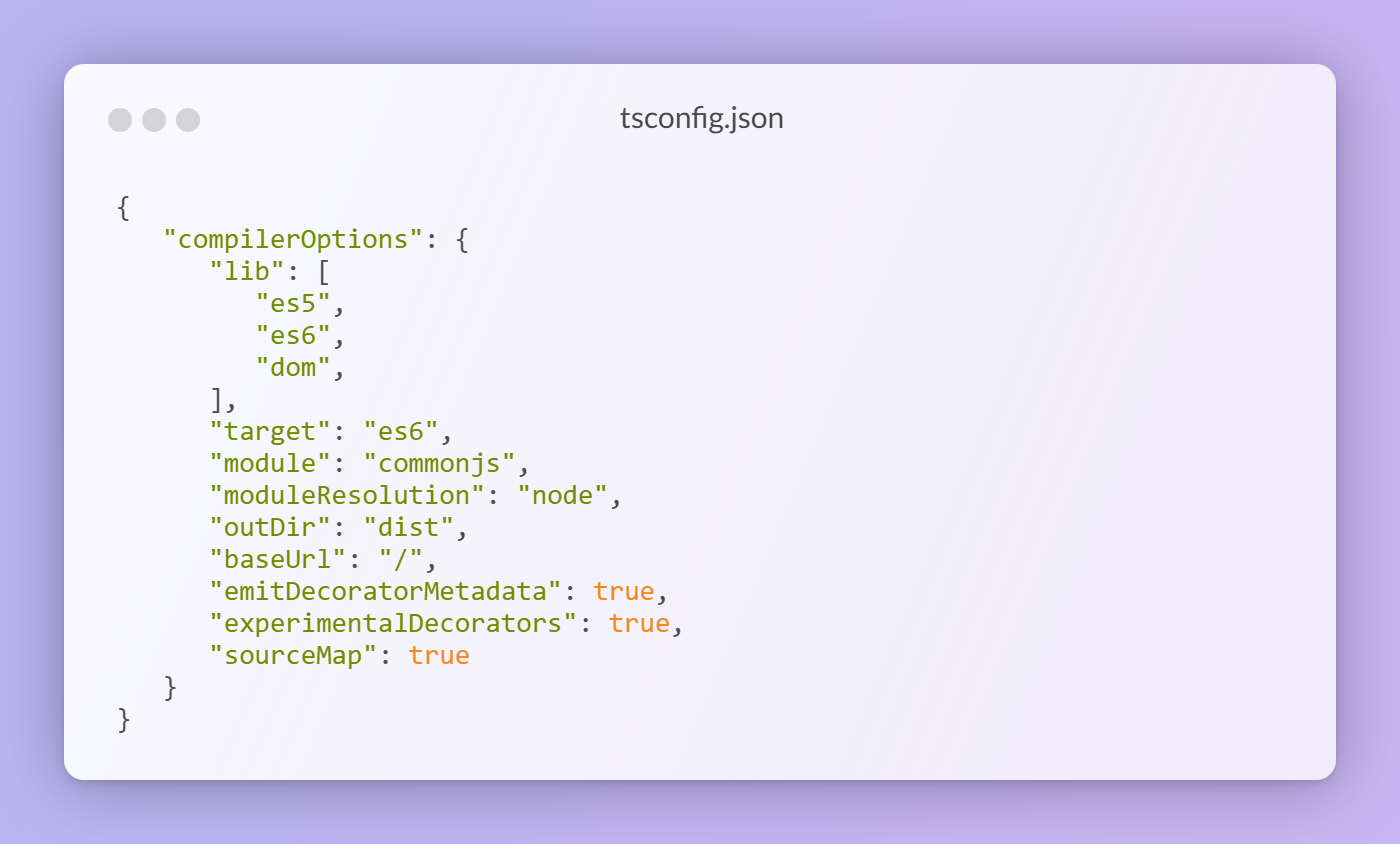
\includegraphics[width=15cm]{assets/presentation/tsjson.png}
    \end{center}
    \caption{Contenu du fichier tsconfig.json}
    \end{figure}

    Les proprietés utilisées dans ce fichier sont les options de compilation de notre projet. L'option \verb|lib| définit les bibliothèques standard disponibles dans notre projet.  (ici es5, es6 et dom). L'option \verb|target| définit la version ECMAScript de sortie (ES6).  La proprieté \verb|module| renseigne sur le système de module (CommonJS pour Node.js), pendant que \verb|moduleResolution| spécifie la résolution des modules (Node.js). \verb|outDir| définit le dossier de sortie (dist). C'est à dire qu'à la compilation, les fichiers en sortis seront mappés dans un dossier "dist"; \verb|baseUrl| définit le chemin de base pour les imports (/). \verb|emitDecoratorMetadata| génère des métadonnées pour les décorateurs; \verb|experimentalDecorators| active les décorateurs (@) ; \verb|sourceMap| permet de debugger avec le code TypeScript

    \vspace{0.35cm}
    
    \item \textbf{Etablir l'architecture du projet} : 

    L'architecture du projet que nous avons établit suit une approche modulaire et structurée, organisée selon les principes de séparation des préoccupations et de maintenabilité. Voici une analyse détaillée de sa structure :

    \begin{description}
        \item[A. Organisation Générale] : 

            La structure racine du projet est organisée en plusieurs dossiers principaux : 

            \begin{itemize}
                \item \verb|/src| : Contient l'ensemble du code source de l'application
                \item \verb|/public| : Héberge les fichiers statiques accessibles publiquement
                \item \verb|/postman| : Stocke les collections Postman pour les tests d'API
                \item \verb|/scripts| : Contient les scripts utilitaires
                \item \verb|/env | : Gère les configurations d'environnement
            \end{itemize}
        
        \item[B. Core de l'Application] :

            Le cœur de l'application \verb|(/src/api/core)| est structuré selon une architecture en couches. L’architecture en couches est un pattern logiciel qui sépare une application en plusieurs couches distinctes, chacune ayant une responsabilité spécifique. Cette architecture permet une meilleure organisation du code, une scalabilité accrue et une facilité de maintenance.

            \begin{description}
                \item[B.1 Couche Présentation] :
                
                Cette couche comprend les \verb|Controllers (/controllers)| organisés par domaine métier.

                \begin{description}
                    \item[-] \verb|auth| :  Gestion de l'authentification
                    \item[-] \verb|catalogs| : Gestion des référentiels
                    \item[-] \verb|communication| : Gestion des communications
                    \item[-] \verb|hr| : Gestion des ressources humaines
                    \item[-] \verb|management| : Gestion des projets
                \end{description}
            \end{description}

            Les contrôleurs sont responsables de :

            \begin{itemize}
                \item La réception des requêtes HTTP
                \item La validation des données entrantes
                \item L'orchestration des appels aux services
                \item La formation des réponses
            \end{itemize}

            \vspace{0.35cm}

            \begin{description}
                \item[B.2 Couche Métier] : 
                    Cette couche comprend les servcies et les dto 
                    \begin{description}
                        \item[- Services (/services)] 
                            Implémentent la logique métier de l'application :
                            
                            \begin{itemize}
                                \item Traitement des données
                                \item Application des règles métier
                                \item Coordination des opérations
                                \item Gestion des transactions
                            \end{itemize}

                        \vspace{0.35cm}
                        \item[- DTOs (/dtos)]
        
                            Définissent les structures de données pour :
                            
                            \begin{itemize}
                                \item Les requêtes entrantes
                                \item Les réponses sortantes
                                \item La validation des données
                            \end{itemize}
                    
                    \end{description}
                \end{description}  
            
            \begin{description}
                \item[B.3 Couche Données] 

                Models (/models) organisés en domaines fonctionnels :

                \begin{verbatim}
/accounts    : Gestion des comptes
/catalogs    : Données de référence
/communication: Modèles de communication
/hr          : Ressources humaines
/management  : Gestion de projet
/media       : Gestion des médias
                \end{verbatim}
            \end{description}
            
            \begin{figure}[H]
            \begin{center}
            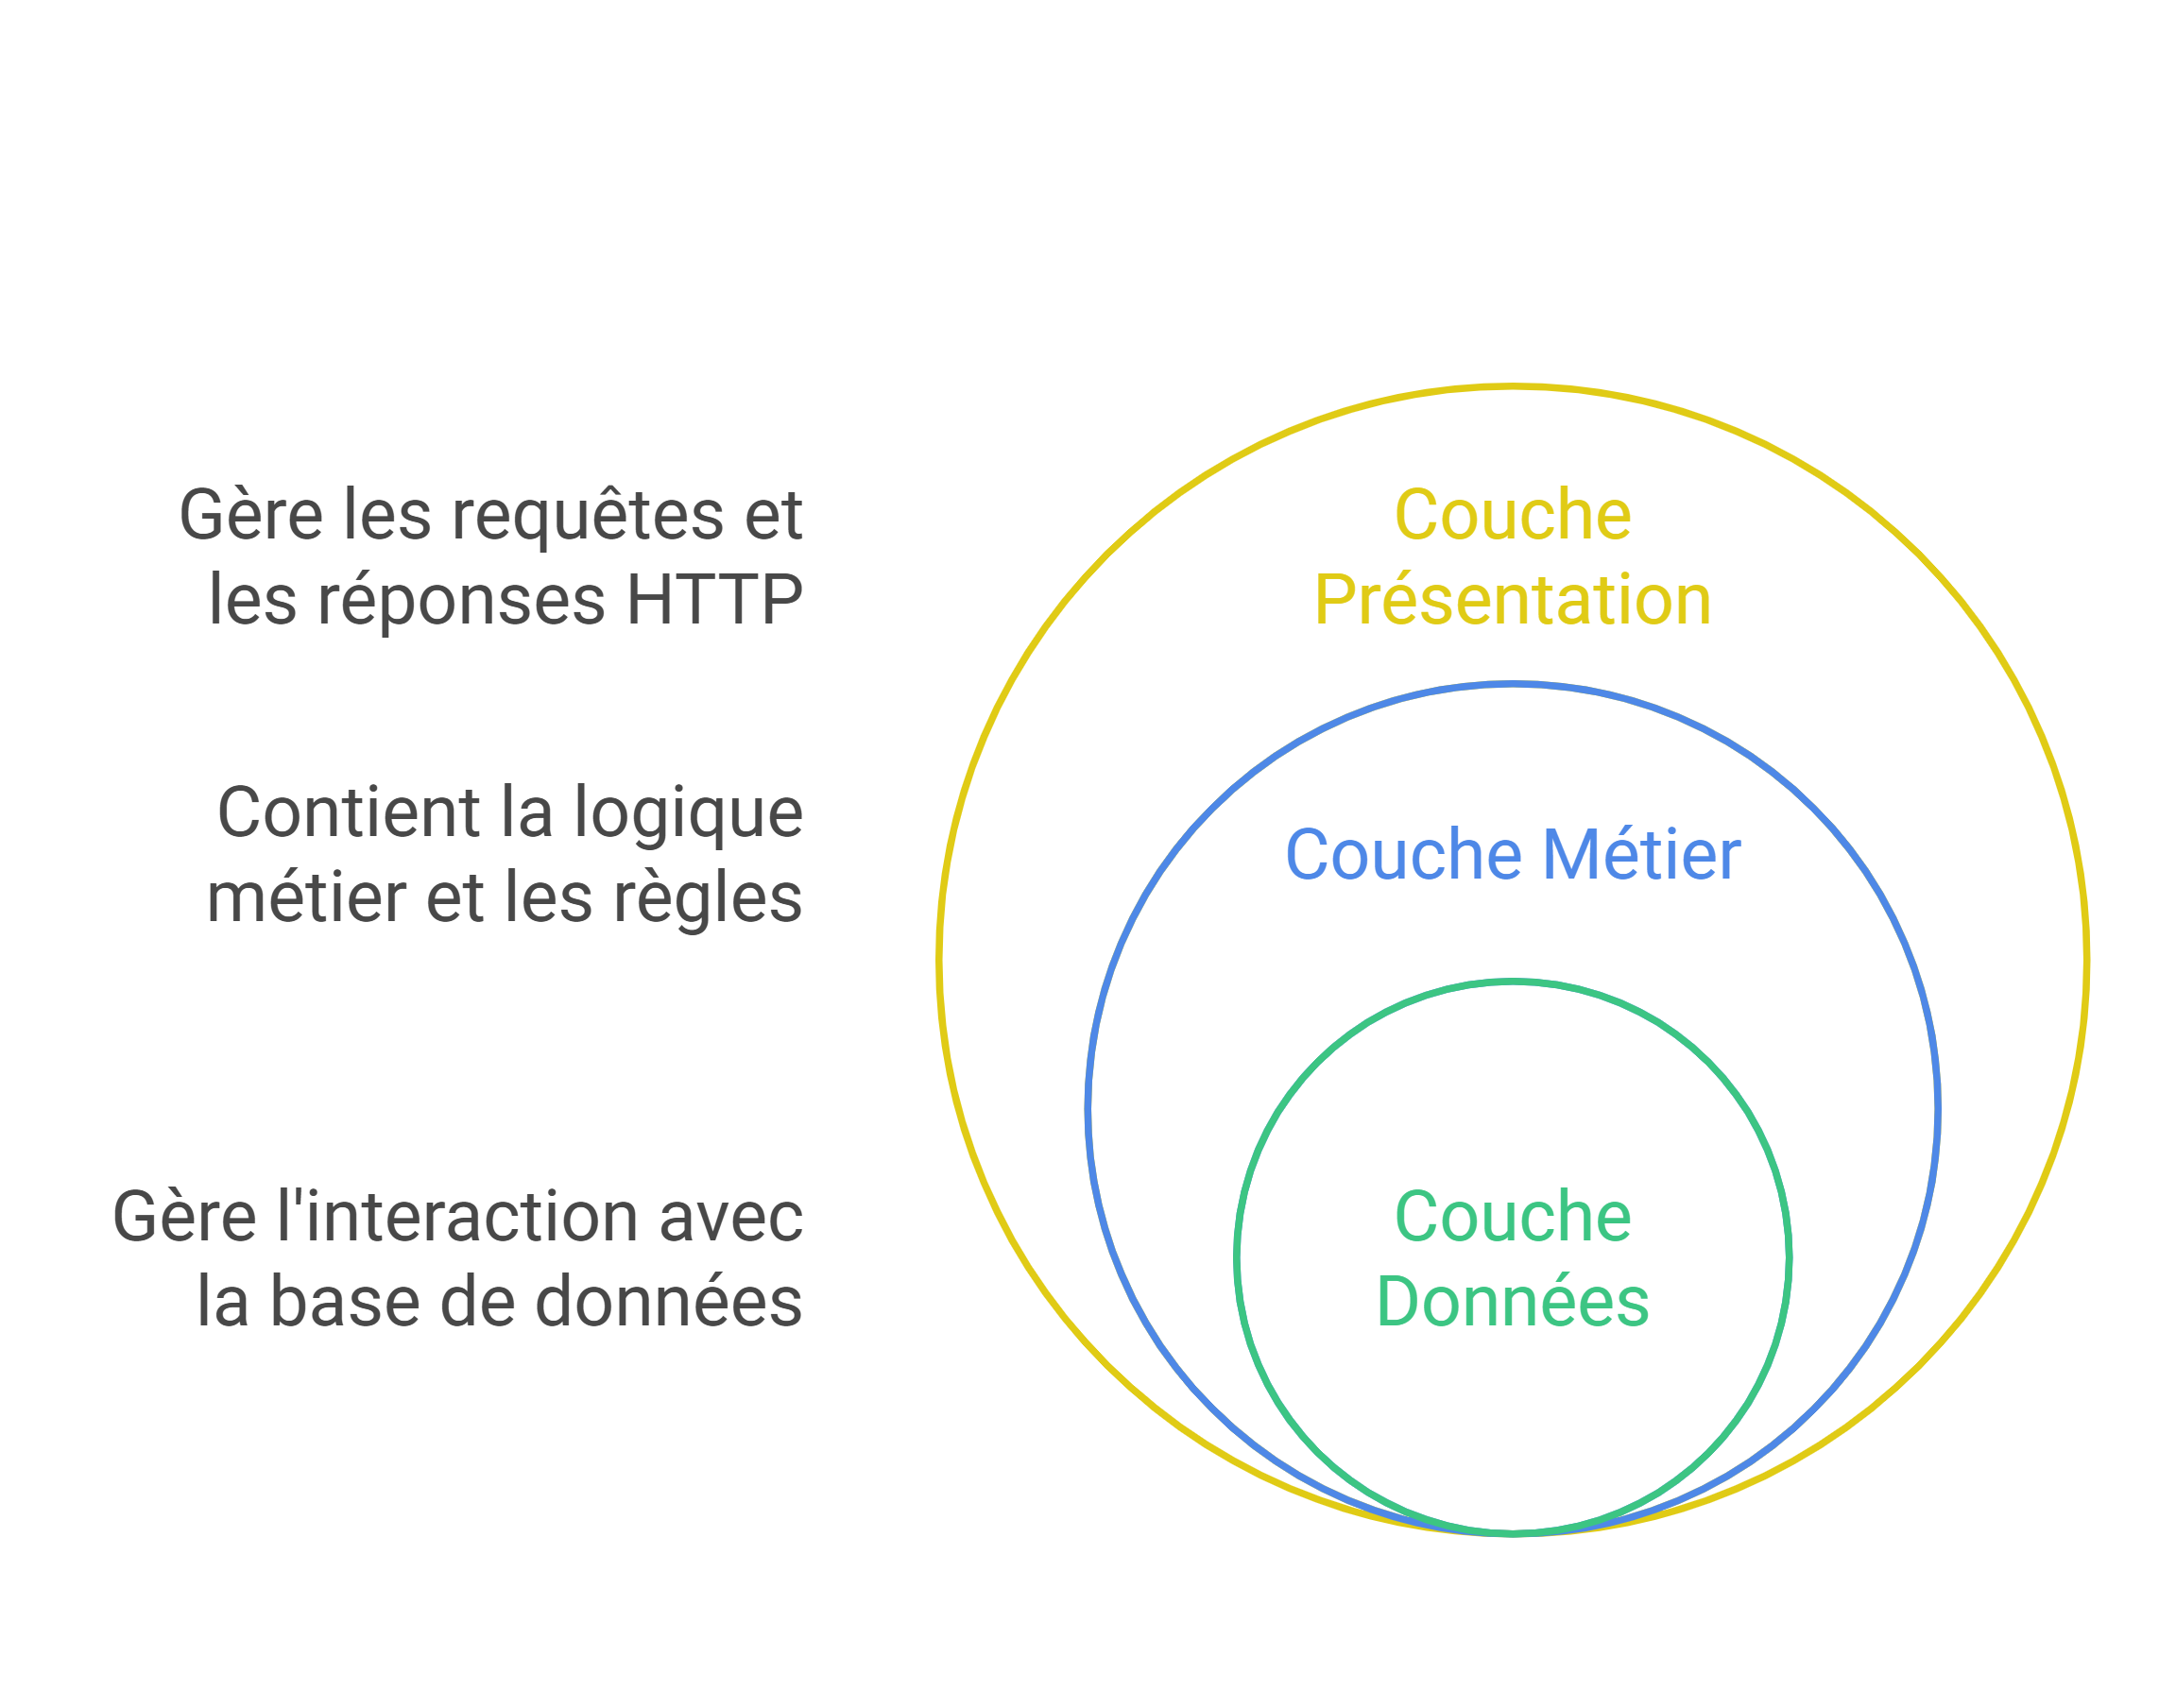
\includegraphics[width=15cm]{assets/presentation/architecture_en_couches.png}
            \end{center}
            \caption{L'architecture en couches ou 3 Layer architecture}
            \end{figure}
            \vspace{0.35cm}

        \item[C. Infrastructure Technique] :

        \begin{description}
            \item[C.1 Configuration] (\verb|/config|)

            Centralise les configurations : 

            \begin{itemize}
                \item Base de données (\verb|database.config.ts|)
                \item Variables d'environnement (\verb|environment.config.ts|)
                \item Authentification (\verb|passport.config.ts|)
                \item Documentation API (\verb|swagger.config.ts|)
                \item Logging (\verb|morgan.config.ts|)
            \end{itemize}

            \item[C.2 Middleware] (\verb|/middlewares|)

            Implémente les fonctionnalités transverses :

            \begin{itemize}
                \item Authentification
                \item Contrôle d'accès (RBAC)
                \item Gestion des uploads
                \item CORS
                \item Géolocalisation IP
            \end{itemize}

            \item[C.3 Types et Interfaces] (\verb|/types|)

            Structure les définitions de types :

            \begin{verbatim}
/classes    : Classes abstraites
/decorators : Décorateurs TypeScript
/enums      : Énumérations
/errors     : Gestion des erreurs
/interfaces : Contrats d'interface
/schemas    : Schémas de validation
            \end{verbatim}
        \end{description}

        \item[D. Fonctionnalités Avancées] :

        \begin{description}
            \item[D.1 Tâches Planifiées] (\verb|/crons|) 
                
            Gère les opérations automatisées :

            \begin{itemize}
                \item Sauvegardes système
                \item Notifications automatiques
                \item Maintenance périodique
            \end{itemize}

            \item[Communication Temps Réel]  (\verb|/sockets|) 

            Implémente les fonctionnalités en temps réel :

            \begin{itemize}
                \item Chat
                \item Notifications
                \item Mises à jour en direct
            \end{itemize}
        \end{description}
Cette architecture est particulièrement adaptée à notre projet car elle permet de disposer de : 

\begin{itemize}
    
    \item Une grande flexibilité
\item Une maintenance à long terme
\item Une évolution progressive
\item Une sécurité renforcée 
\end{itemize}

\vspace{0.35cm}
    
La structure adoptée facilite également l'intégration de nouvelles fonctionnalités et l'adaptation aux évolutions des besoins métiers.

\end{description}

Comme illustré dans l'image ci-dessous, l'architecture du projet s'articule autour d'un point d'entrée central situé à la racine du cœur de l'application (\verb|src/api/core|). Le fichier \verb|app.bootstrap.ts| constitue le point de démarrage de l'application et joue un rôle fondamental dans l'initialisation et le montage des différents composants.

\vspace{0.35cm}

Ce fichier bootstrap remplit plusieurs fonctions essentielles :

\begin{enumerate}
    \item Initialisation du serveur Express et configuration des middlewares de base
    \item Chargement des variables d'environnement et des configurations
    \item Établissement des connexions aux services externes (base de données, cache, etc.)
    \item Montage des routes de l'API
    \item Configuration des gestionnaires d'erreurs globaux
\end{enumerate}

\vspace{0.35cm}

\begin{figure}[H]
\begin{center}
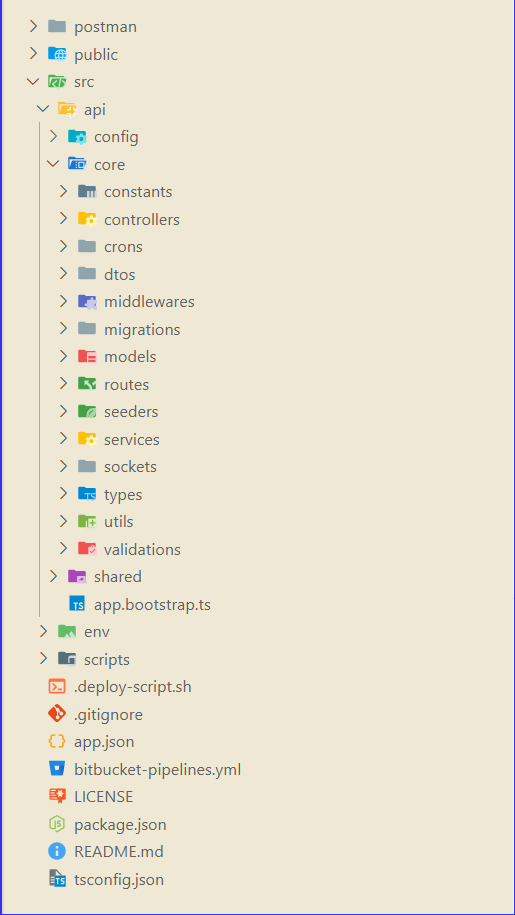
\includegraphics[width=10cm]{assets/presentation/treewh.png}
\end{center}
\caption{Architecture du projet backend}
\end{figure}

\vspace{0.35cm}

La centralisation de ces responsabilités dans un fichier bootstrap unique permet :

\begin{itemize}
    \item Une séquence de démarrage claire et maîtrisée
    \item Une gestion cohérente des dépendances
    \item Un point unique de configuration de l'application
    \item Une meilleure maintenabilité du code
\end{itemize}

Une fois que l'architecture du projet est établie, il est nécessaire d'établir toutes les configurations inhérentes au projet et s'assurer qu'elles fonctionnent. Ensuite, on peut commencer par implémenter les classes dont les relations ont été définies plus haut.

\end{enumerate}

\subsubsection*{Limites de l'architecture et des choix technologiques}
Bien que l'architecture en couches et les choix technologiques adoptés présentent de nombreux avantages, il est important de noter certaines limitations dans le contexte spécifique du projet Fixaars :

\begin{enumerate}
    \item \textbf{Complexité de la structure} : 
    \begin{itemize}
        \item L'architecture en couches, bien que modulaire, peut introduire une complexité accrue pour les développeurs juniors qui rejoignent le projet
        \item La multiplication des dossiers et sous-dossiers peut ralentir le développement de nouvelles fonctionnalités, notamment pour les cas d'usage simples
        \item Le découpage strict en couches peut parfois sembler artificiel pour certaines fonctionnalités basiques de gestion
    \end{itemize}

    \item \textbf{Performance} :
    \begin{itemize}
        \item L'utilisation de TypeORM, bien que facilitant le développement, peut introduire une surcharge de performance comparé à des requêtes SQL optimisées manuellement
        \item La structure en couches multiplie les transformations de données (DTO → Service → Model), ce qui peut impacter les performances pour les opérations à haute fréquence
        \item Le choix de Node.js monothread peut limiter les performances pour les calculs intensifs liés à la gestion des emplois du temps
    \end{itemize}

    \item \textbf{Défis spécifiques à Fixaars} :
    \begin{itemize}
        \item Le modèle de données fortement relationnel de Fixaars (liens entre employés, missions, plannings) peut créer des problèmes de performance avec TypeORM pour les requêtes complexes
        \item La séparation stricte des couches peut compliquer l'implémentation de certaines règles métier spécifiques au secteur des services à la personne
        \item L'architecture actuelle pourrait nécessiter des adaptations pour supporter efficacement la gestion des cas exceptionnels fréquents dans les services à la personne (annulations de dernière minute, remplacements urgents)
    \end{itemize}
\end{enumerate}

Ces limitations ne remettent pas en cause la pertinence globale des choix architecturaux, mais soulignent des points d'attention pour l'évolution future du projet. Certaines de ces limitations pourraient être adressées par :
\begin{itemize}
    \item L'introduction de caching intelligent pour les données fréquemment accédées
    \item L'optimisation ciblée des requêtes TypeORM critiques
    \item La mise en place de documentation approfondie des patterns d'utilisation
    \item L'adoption progressive de microservices pour les fonctionnalités critiques en termes de performance
\end{itemize}

\subsection*{Présentation technique du frontend}
Le projet frontend suit aussi la stack technologique \verb|javascript|. Nous avons utilisé du \verb|Javascript|, \verb|TypeScript|, \verb|Node.js| et \verb|Express.js|. Le moteur de template utilisé dans ce projet est \verb|EJS| (Embedded JavaScript)

\vspace{0.35cm}

Un moteur de template est un outil qui permet de générer du HTML (ou d'autres formats) à partir de modèles (ou templates) qui contiennent des éléments dynamiques. Ces moteurs sont largement utilisés dans le développement web pour séparer la logique de présentation du contenu et de la gestion des données. \verb|EJS| (Embedded JavaScript) est un moteur de templates pour JavaScript, principalement utilisé avec des applications Node.js, en particulier avec des frameworks comme Express. Il permet de générer dynamiquement du HTML côté serveur en insérant des données dans les templates.

\vspace{0.35cm}

Les étapes de mise en place du projet sont pratiquement les mêmes qu'avec le backend. Seulement, dans ce cas-ci, Lors de la configuration technique du projet, il faut s'assurer de spécifier le moteur de template du projet. Il faut également ajouter au projet un dossier qui sera considéré comme dossier de base pour les template : il s'agit du dossier \verb|views|. 

\vspace{0.35cm} 
Dans un projet Express avec EJS, un dossier \verb|views| sert à stocker les fichiers de templates EJS. Ces fichiers sont utilisés pour générer du HTML dynamique côté serveur, en intégrant des données envoyées depuis le serveur dans la vue avant d'être envoyées au client.

\vspace{0.35cm}

\begin{figure}[H]
\begin{center}
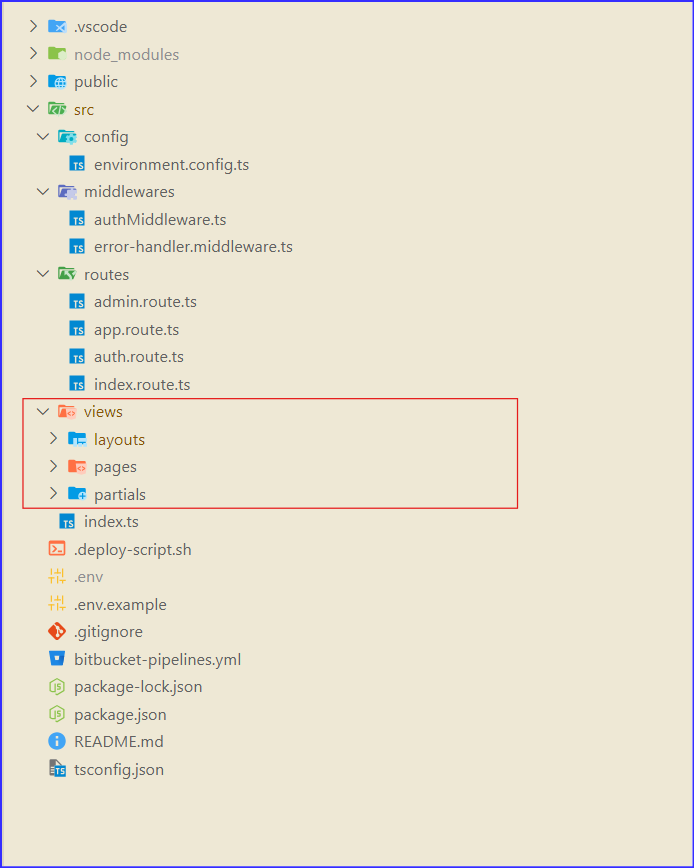
\includegraphics[width=10cm]{assets/presentation/fixaars-front.png}
\end{center}
\caption{Architecture du projet frontend}
\end{figure}

L'encadré rouge sur la photo précédente montre le dossier des vues de notre projet \verb|views|. Ce dossier contient les sous-dossiers suivants : 

\begin{itemize}
    \item \textbf{layouts} : contient les principaux layouts de notre application qui sont inclus dans les autres pages pour éviter la répétition du code (en utilisant par exemple \verb|<%- include('header') %>| ).
    \item \textbf{pages} : contient toutes les pages de notre applications
    \item \textbf{partials} : contient les vues partagées (comme des formulaires ou des listes) réutilisables dans d'autres pages. Cela rend l'application plus modulaire et facilite la gestion du code.
\end{itemize}

\vspace{0.35cm}

EJS utilise des fichiers de template (généralement avec l'extension \verb|.ejs|), qui ressemblent à des fichiers HTML classiques, mais qui contiennent des balises EJS permettant d'incorporer du code JavaScript et de manipuler des données.

\vspace{0.35cm}

\begin{figure}[H]
\begin{center}
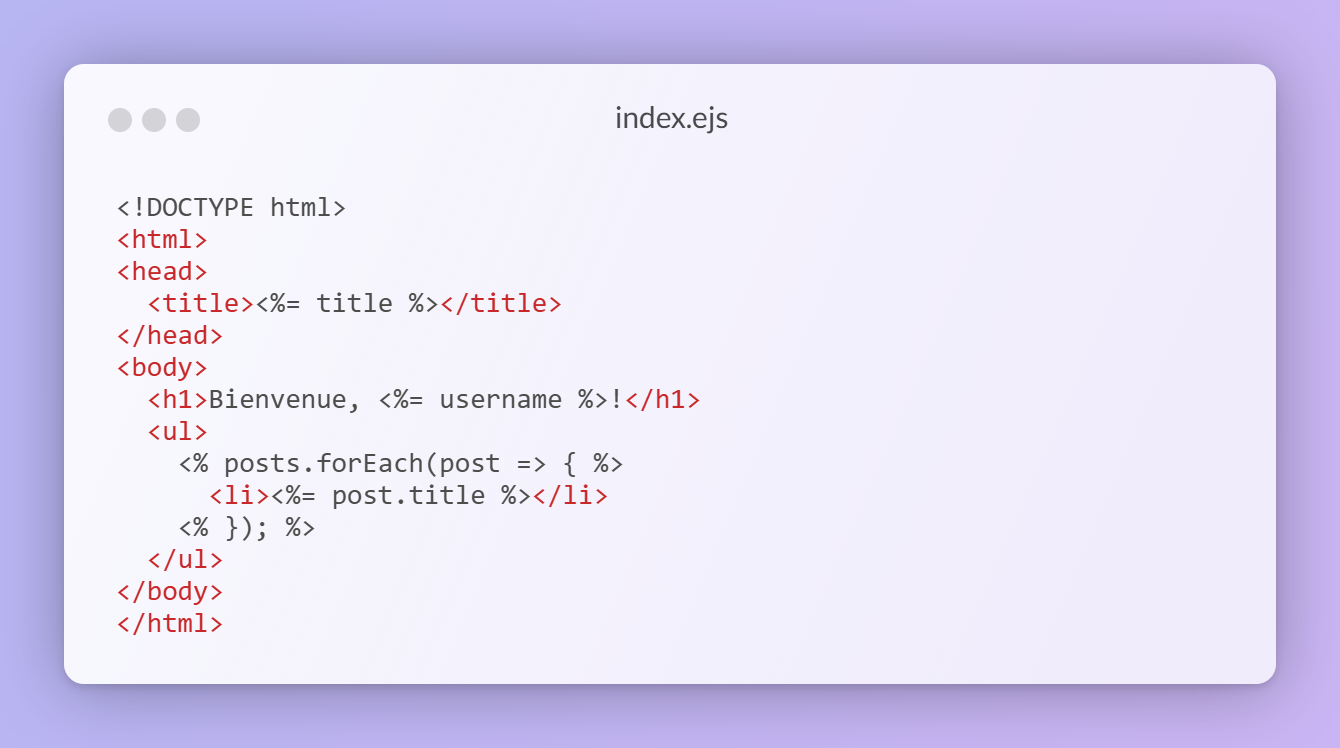
\includegraphics[width=15cm]{assets/presentation/ejs-snippet.png}
\end{center}
\caption{Exemple simple de fichier .ejs}
\end{figure}

\vspace{0.35cm}

\begin{itemize}
    \item \verb|<%= title %>| : Affiche la valeur de la variable "title".
    \item \verb|<%= username %>| : Affiche la valeur de la variable "username".
    \item \verb|<% posts.forEach(...) %>| : Exécute une boucle JavaScript pour afficher une liste de "posts".
\end{itemize}

\vspace{0.35cm}

Pour utiliser cette vue dans une application express, il faut configurer EJS comme moteur de vues et lui passer des données pour générer dynamiquement le contenu des pages.

\newpage

\begin{figure}[H]
\begin{center}
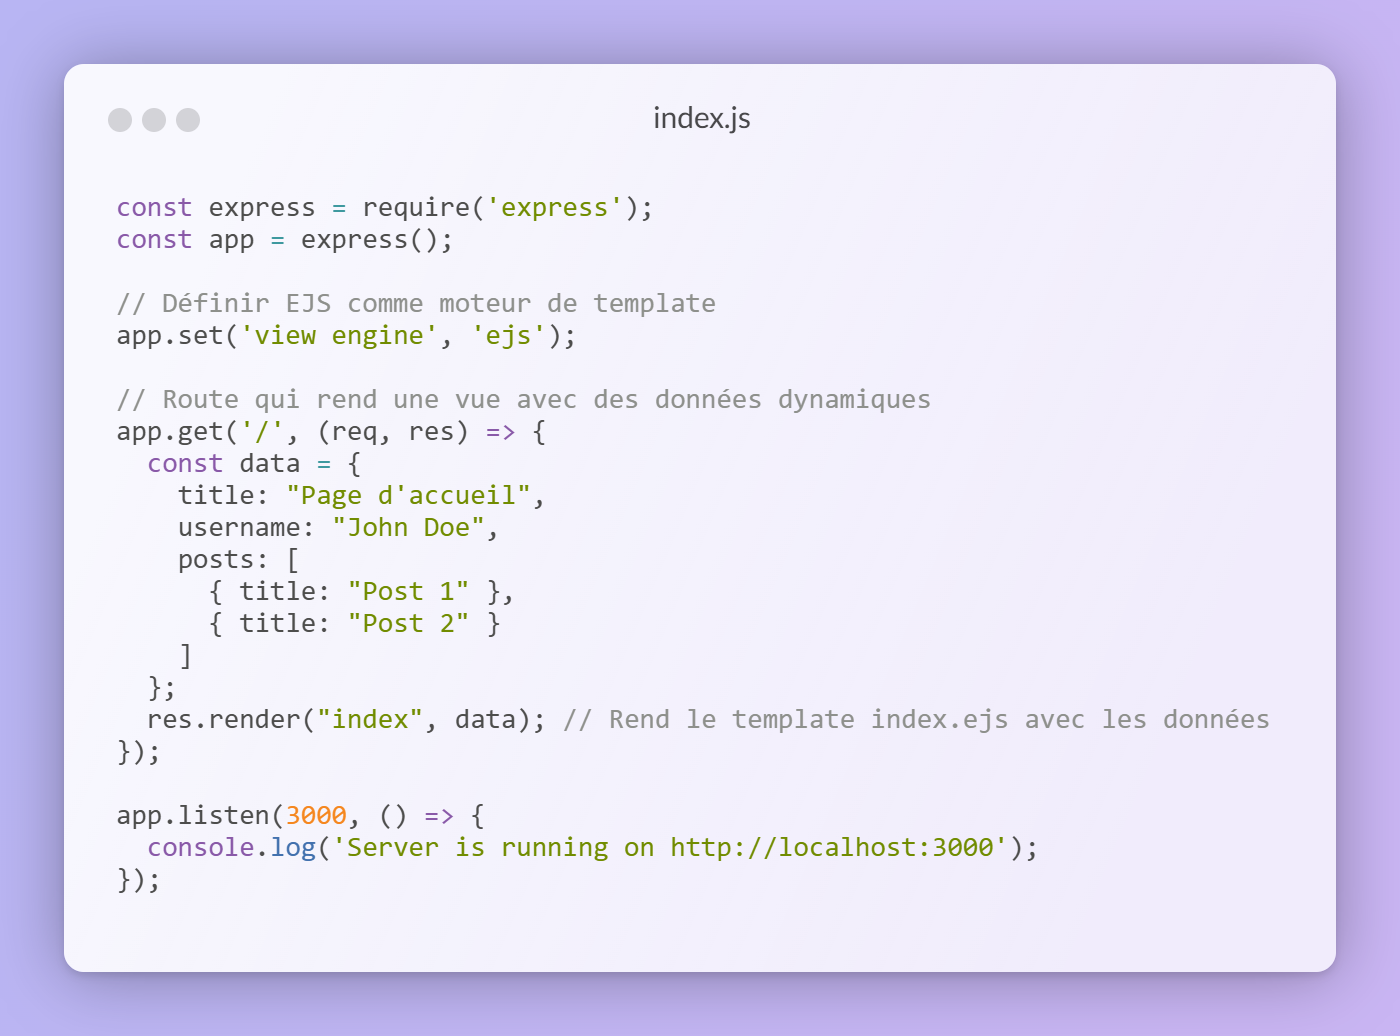
\includegraphics[width=15cm]{assets/presentation/ejs2-snippet.png}
\end{center}
\caption{Exemple simple de fichier .js}
\end{figure}


\section{Présentation Fonctionnelle de l'application}

Cette partie présente avec support visuel quelques-unes des interfaces implémentées dans le cadre de ce projet. 

\subsection{Landing Page}

Lorsque l'utilisateur entre l'adresse fixaars dans sa barre de recherche, il est redirigé sur la page d'accueil de l'application. 

\vspace{1cm}

Cette page d'accueil, comme illustrée sur la figure suivante se présente sous diverses sections bien spécifiques. L'utilité de cette page est de fournir un accès rapide avec l'information minimum pour un utilisateur de prendre rapidement en main l'outil. 


%galerie d'image
\begin{figure}[htp]
  \centering
  \subfloat[Header \& Barre de recherche]{\label{fig:première}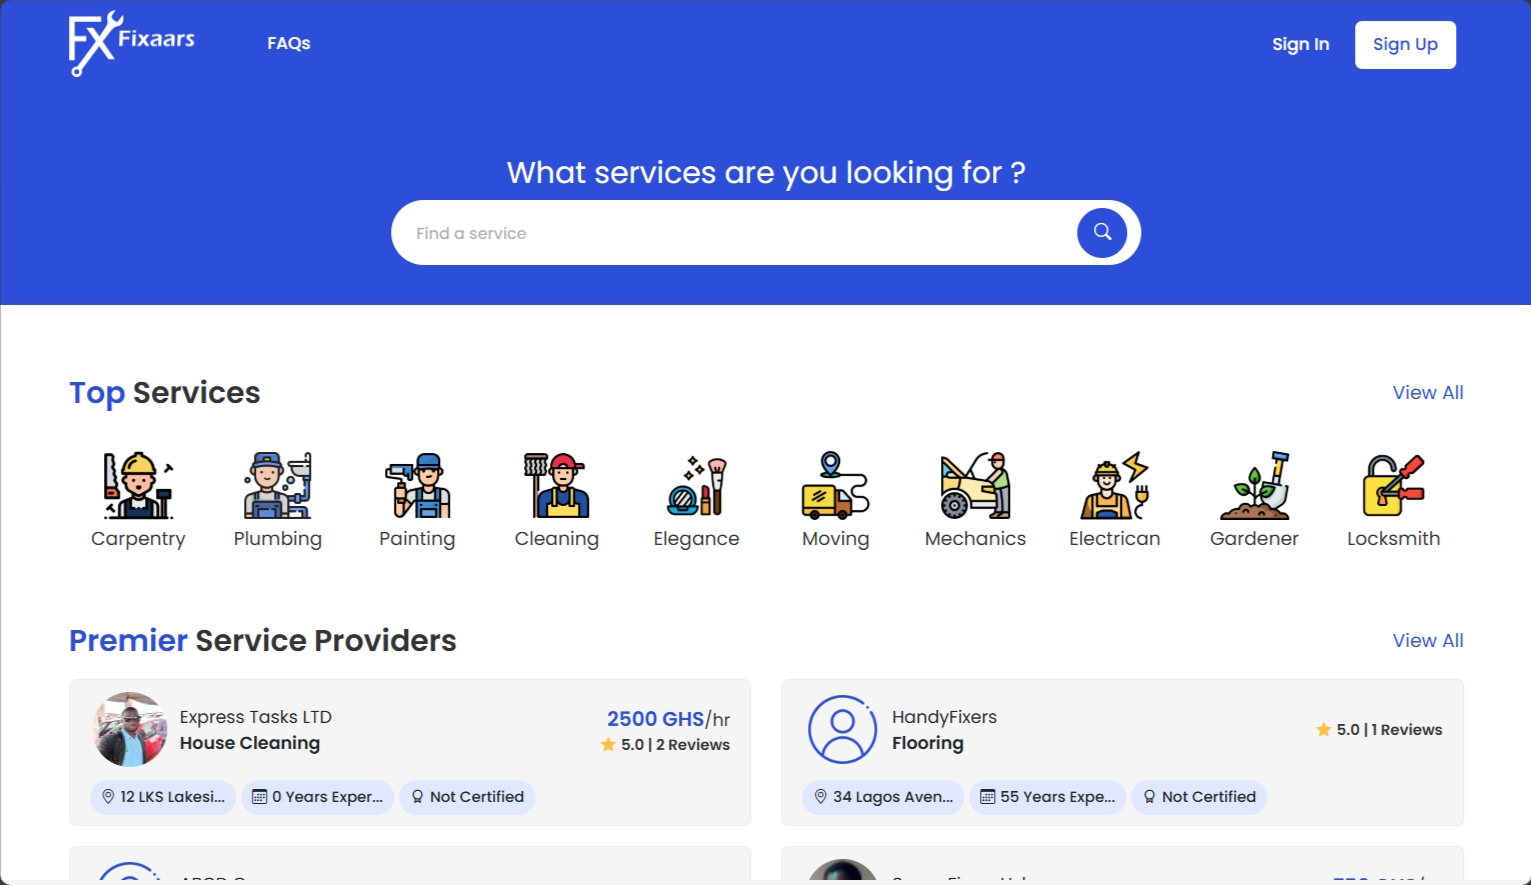
\includegraphics[width=9cm]{assets/demo/landing-1.png}}
  ~ %espace entre deux images sur une même ligne
  \subfloat[Services en Vogues sur Fixaars]{\label{fig:deuxième}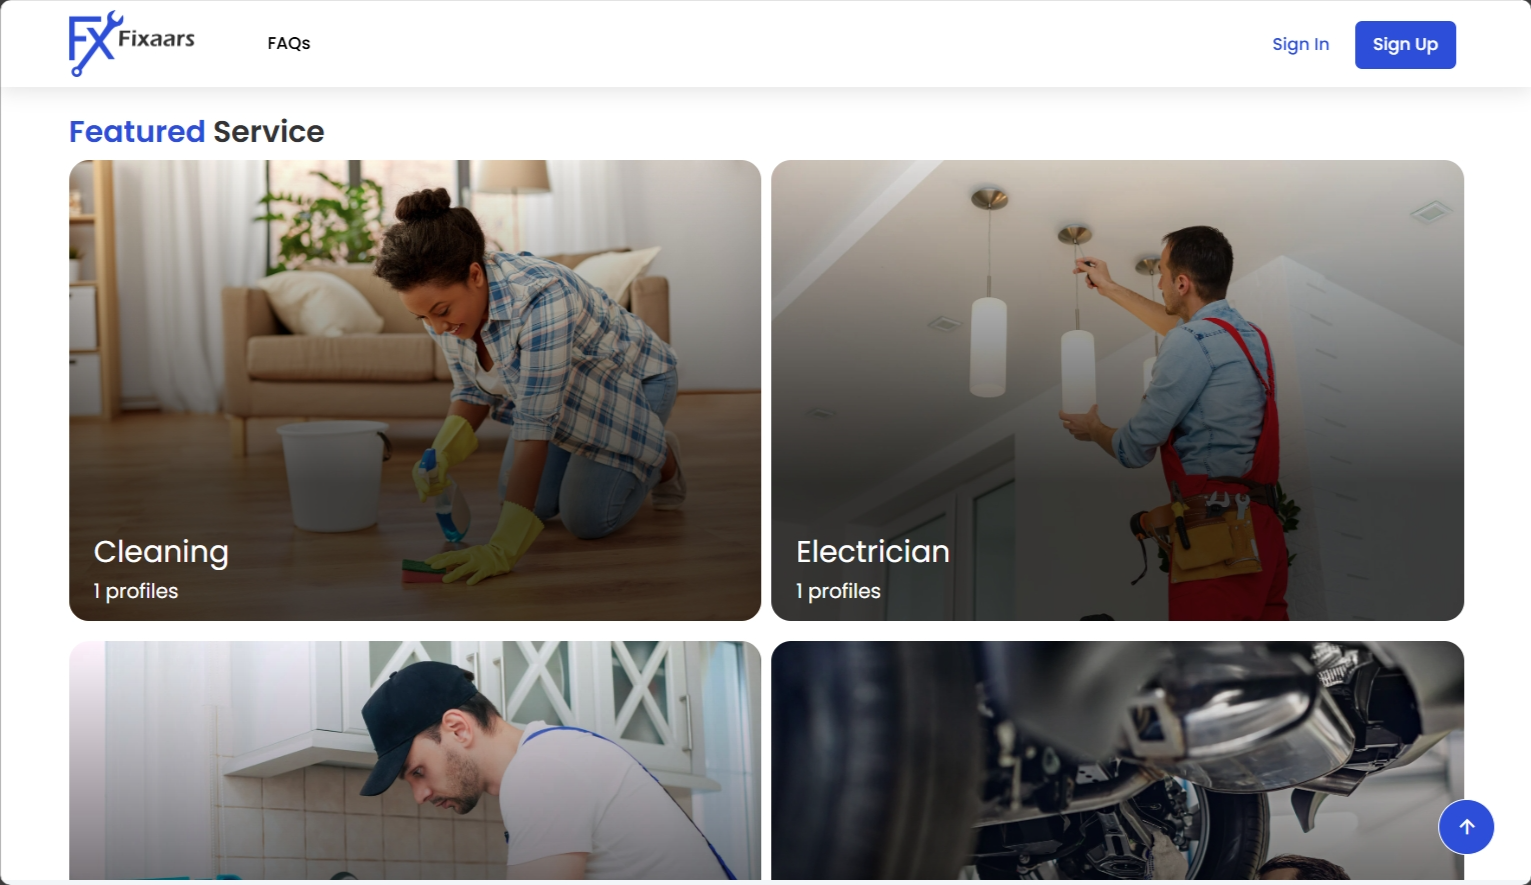
\includegraphics[width=9cm]{assets/demo/landing-2.png}}
  ~\\
    \subfloat[Comment ça marche ?]{\label{fig:troisième}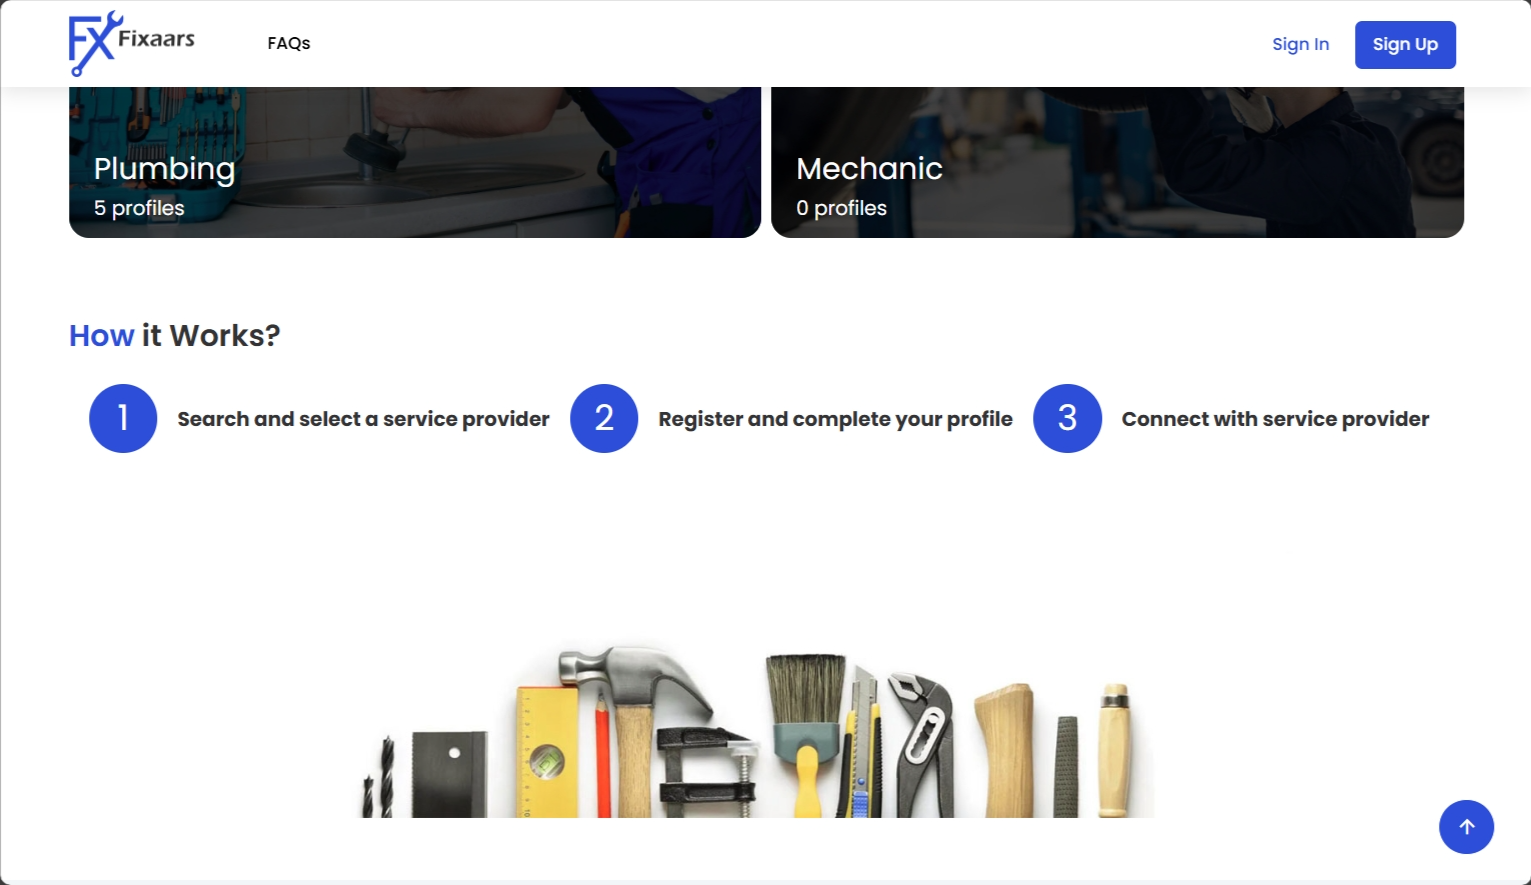
\includegraphics[width=9cm]{assets/demo/landing-3.png}}
  ~ %espace entre deux images sur une même ligne
  \subfloat[Avis \& Recommandations]{\label{fig:quatrième}
\includegraphics[width=9cm]{assets/demo/landing-4.png}}
  ~\\ %saute une ligne dans la galerie d'image
  \subfloat[Footer]{\label{fig:cinquième}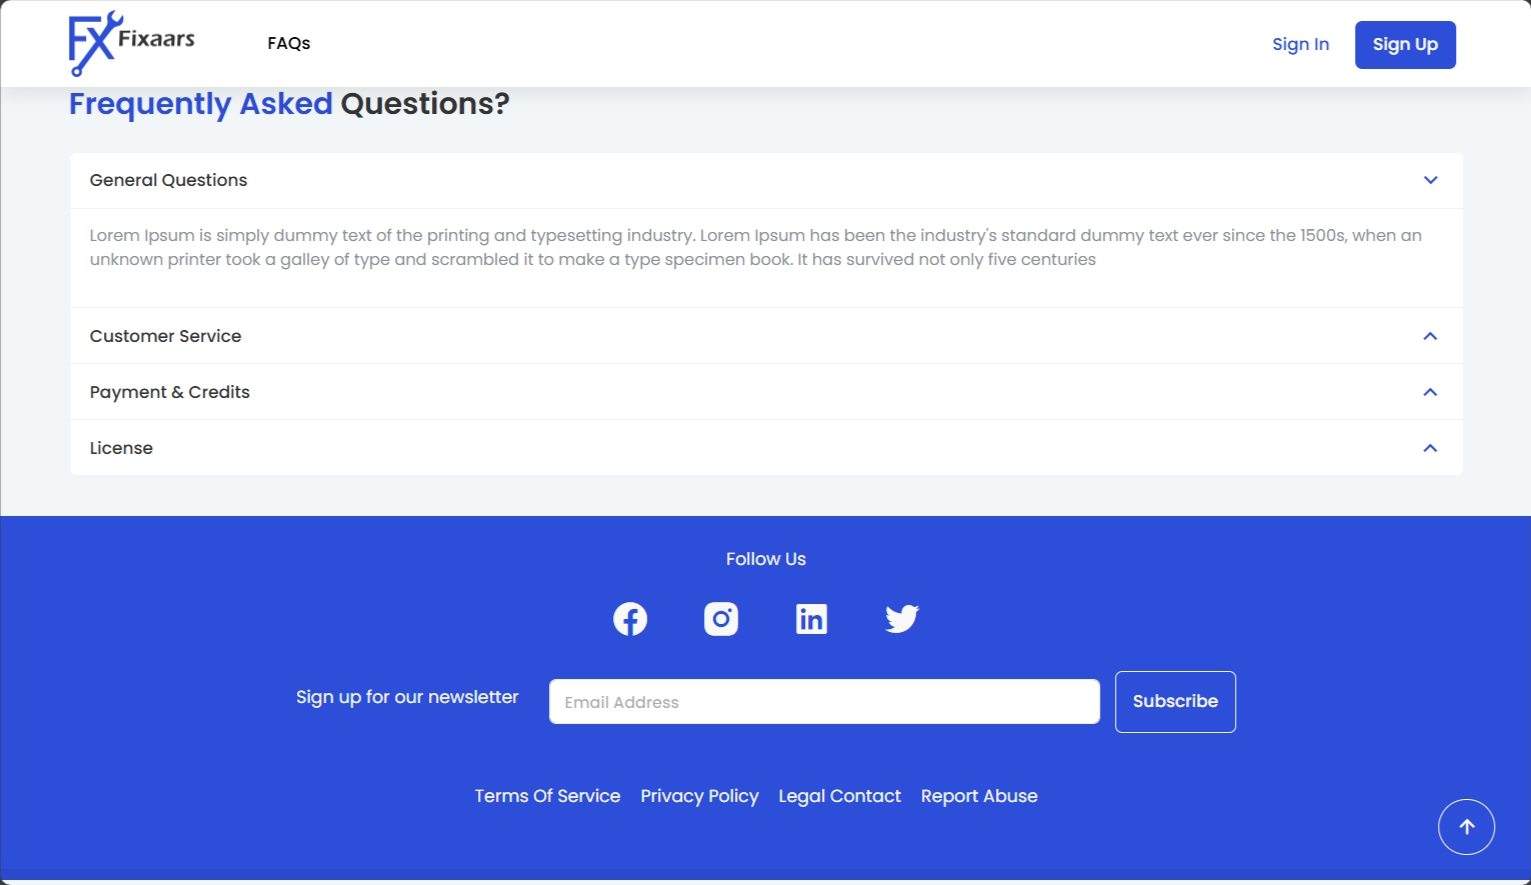
\includegraphics[width=9cm]{assets/demo/landing-5.png}}
  \caption{Différentes captures de la page d'accueil}
  \label{fig:gallerieLanding}
\end{figure}

\newpage

\subsection{Pages d'authentification}

Pour s'authentifier, l'utilisateur utilise la page de login ci-dessous

\begin{figure}[H]
\begin{center}
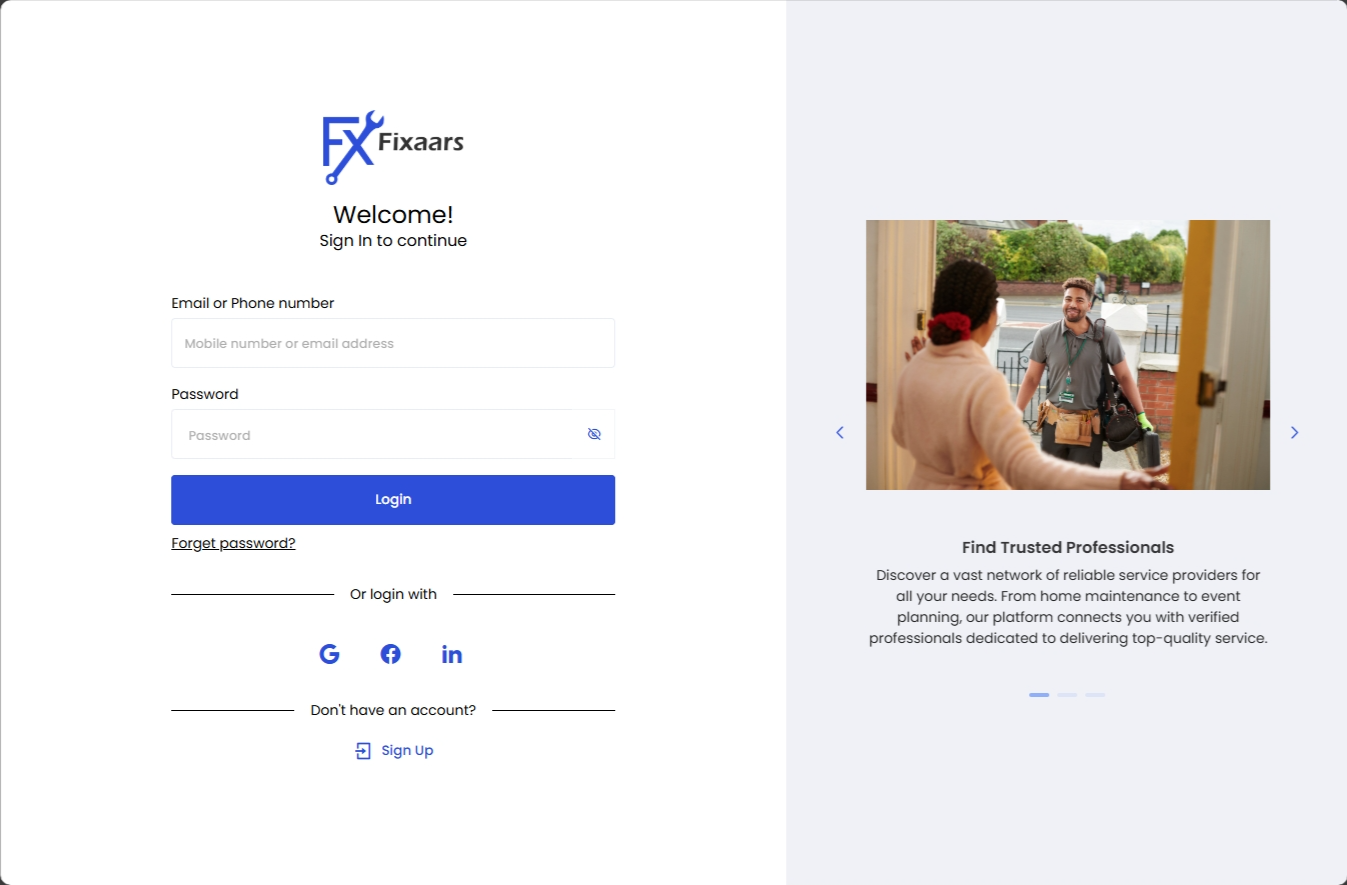
\includegraphics[width=12cm]{assets/demo/login.png}
\end{center}
\caption{Page de Login}
\end{figure}

L'enregistrement se fait sur la page suivante

\begin{figure}[H]
\begin{center}
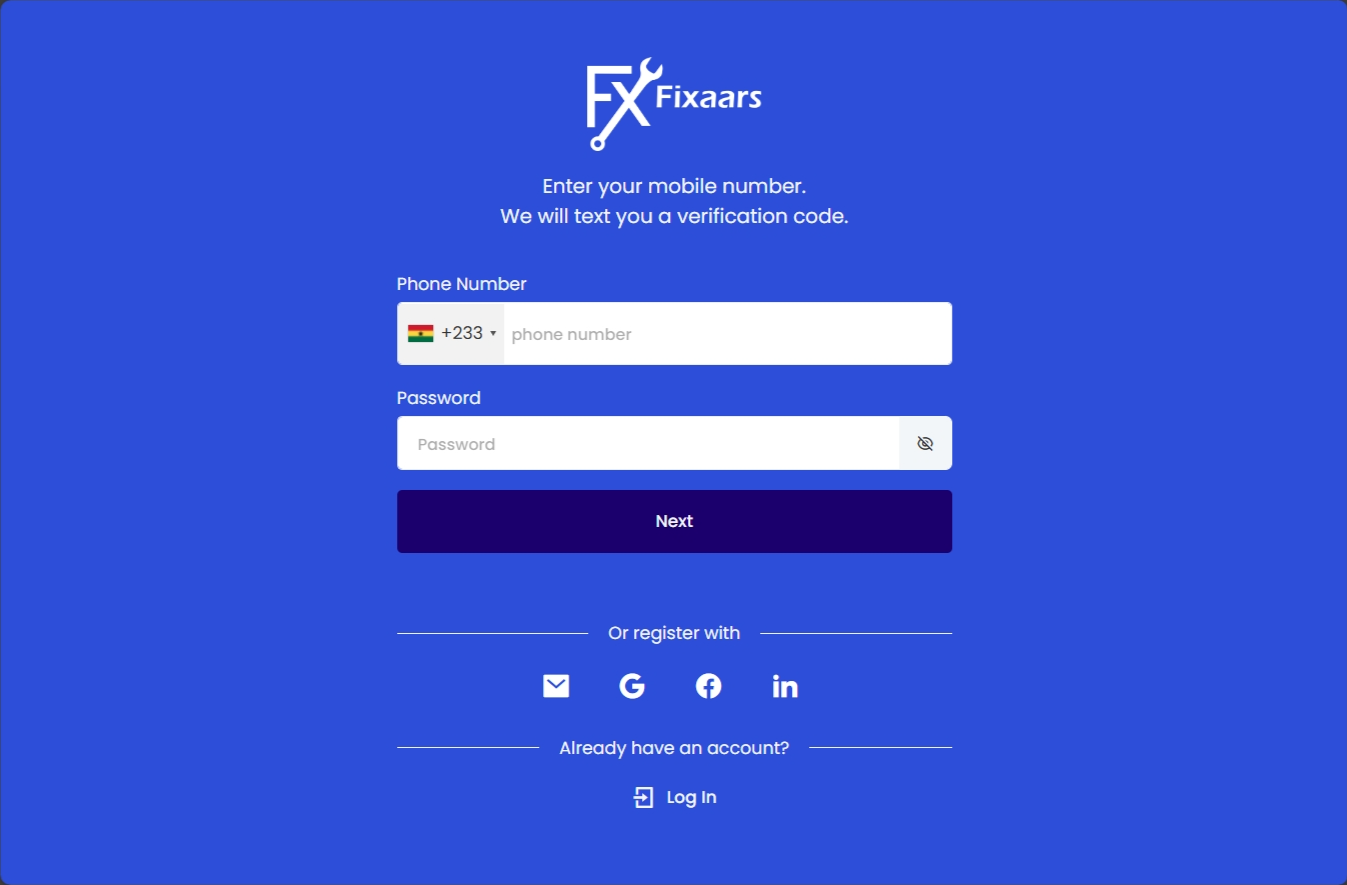
\includegraphics[width=12cm]{assets/demo/signup.png}
\end{center}
\caption{Page d'enregistrement}
\end{figure}

Comme indiqué sur l'image, plusieurs moyens d'authentification et d'enregistrement sont disponibles sur la plateforme : Email et mot de passe (authentification classique), Authentification Google, Authentification Facebook, Authentification LinkedIn.

\vspace{0.35cm}

L'enregistrement sur la plateforme se fait en deux étapes : L'étape 1 consiste à entrer ses informations basique ou juste cliquer sur une des solutions d'authentifications supportée par la plateforme.

\begin{figure}[H]
\begin{center}
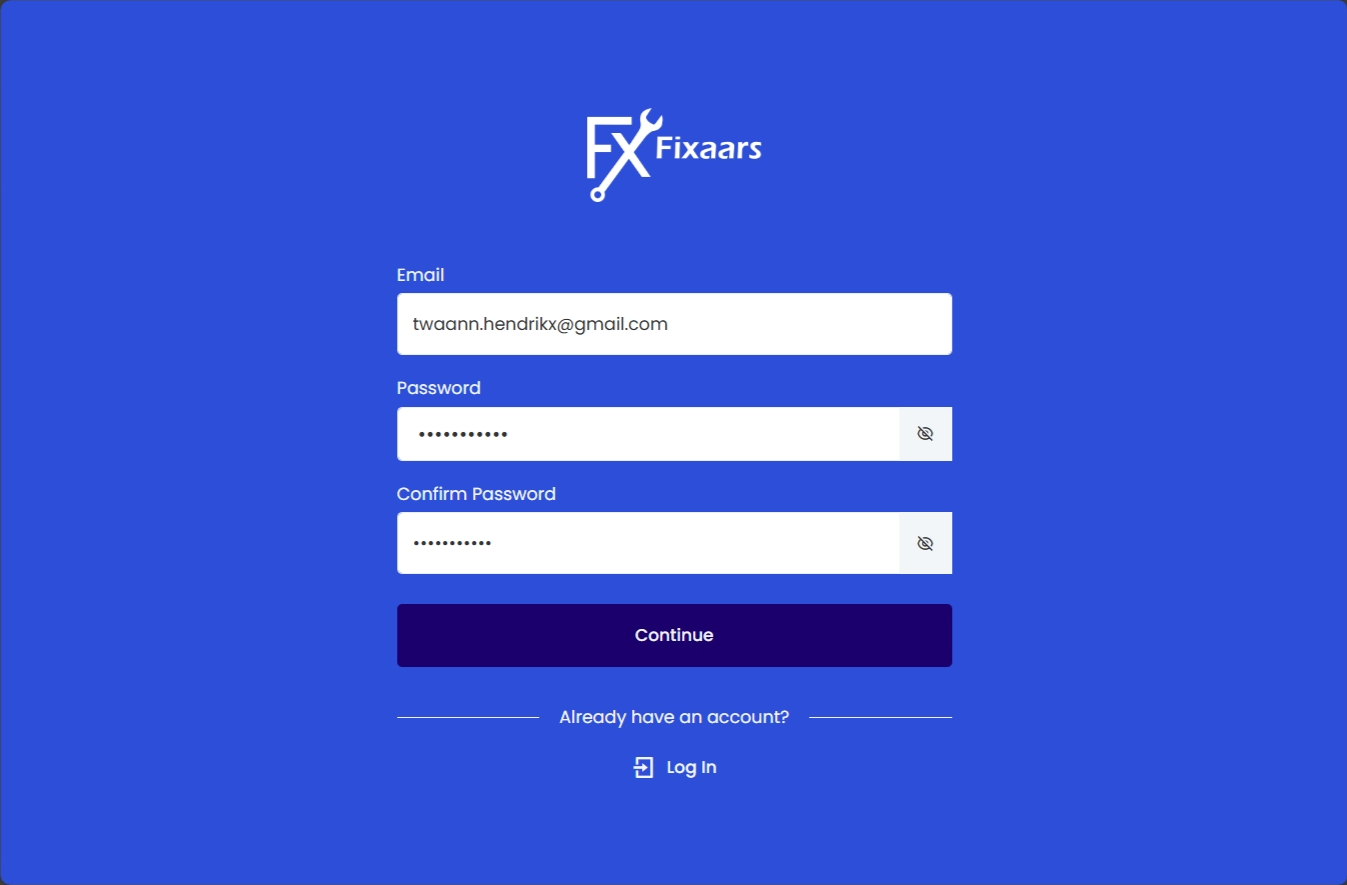
\includegraphics[width=12cm]{assets/demo/signup-email.png}
\end{center}
\caption{Page d'enregistrement - Etape 1}
\end{figure}

Ensuite, une fois cette étape validée, l'utilisateur devra compléter ses informations en précisant son rôle sur la plateforme : (Customer ou Business).

\begin{figure}[H]
\begin{center}
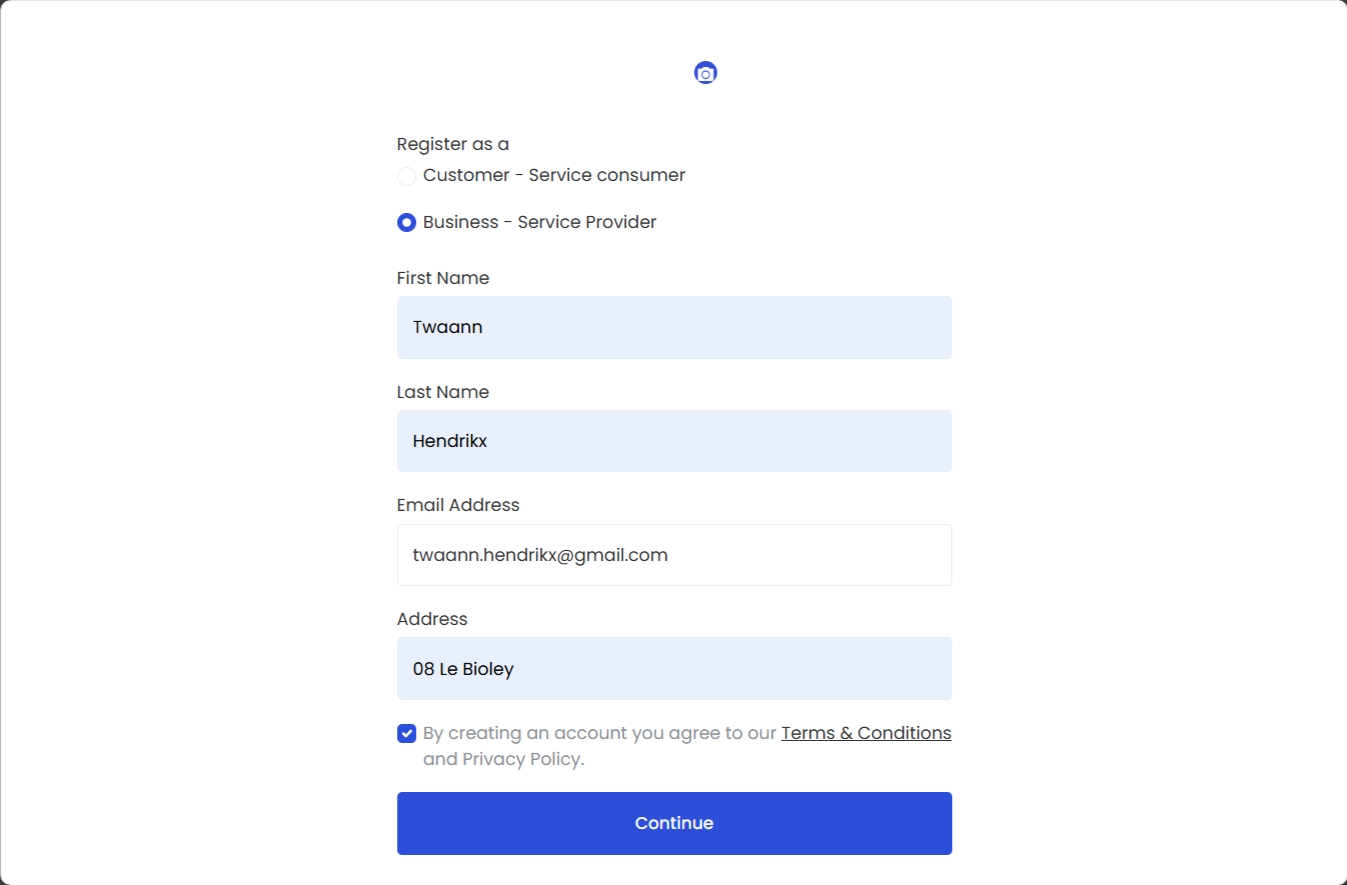
\includegraphics[width=12cm]{assets/demo/signup-2.png}
\end{center}
\caption{Page d'enregistrement - Etape 2}
\end{figure}

Une fois ce processus terminé, l'utilisateur est authentifié automatiquement et redirigé sur l'écran d'accueil en fonction de son rôle. S'il est Business, il aura un écran d'accueil similaire à ceci :

\vspace{0.35cm}
\begin{figure}[H]
\begin{center}

\includegraphics[width=12cm]{assets/demo/sp1.png}
\end{center}
\caption{Page d'enregistrement - Etape 2}
\end{figure}

\subsection{Recherche de prestataires de services}

Pour faire la recherche de prestataires de services, l'utilisateur peut entrer sur son écran d'accueil le nom du service pour lequel il recherche un prestataire. Il lui sera fournie une page similaire à celle-ci  :

\vspace{0.35cm}
\begin{figure}[H]
\begin{center}
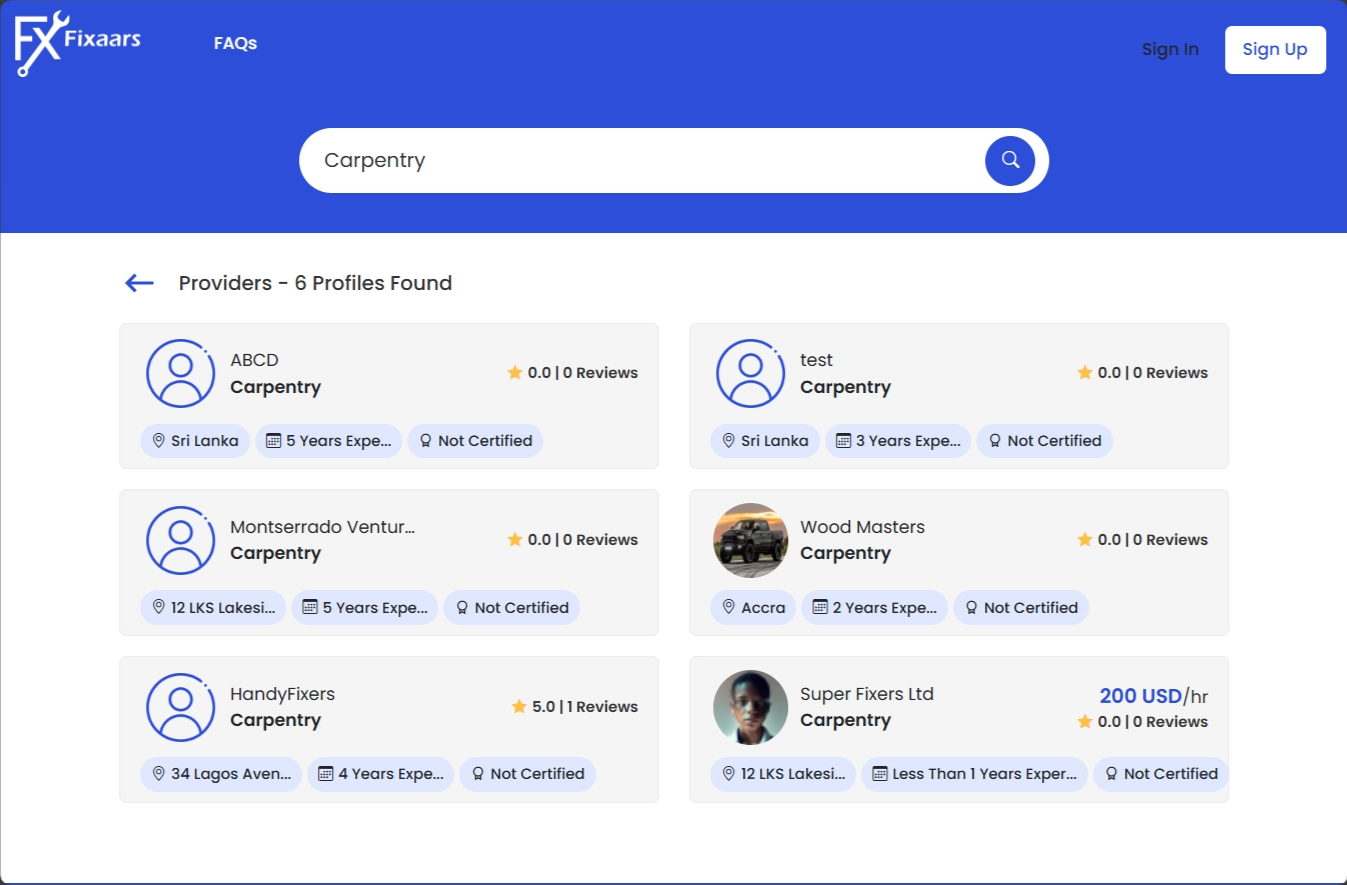
\includegraphics[width=12cm]{assets/demo/search-1.png}
\end{center}
\caption{Page de Recherche}
\end{figure}

S'il n'est pas encore authentifié, il ne pourra pas voir les détails du profil. Il sera invité à s'authentifier avant de continuer le processus.

\vspace{0.35cm}
\begin{figure}[H]
\begin{center}
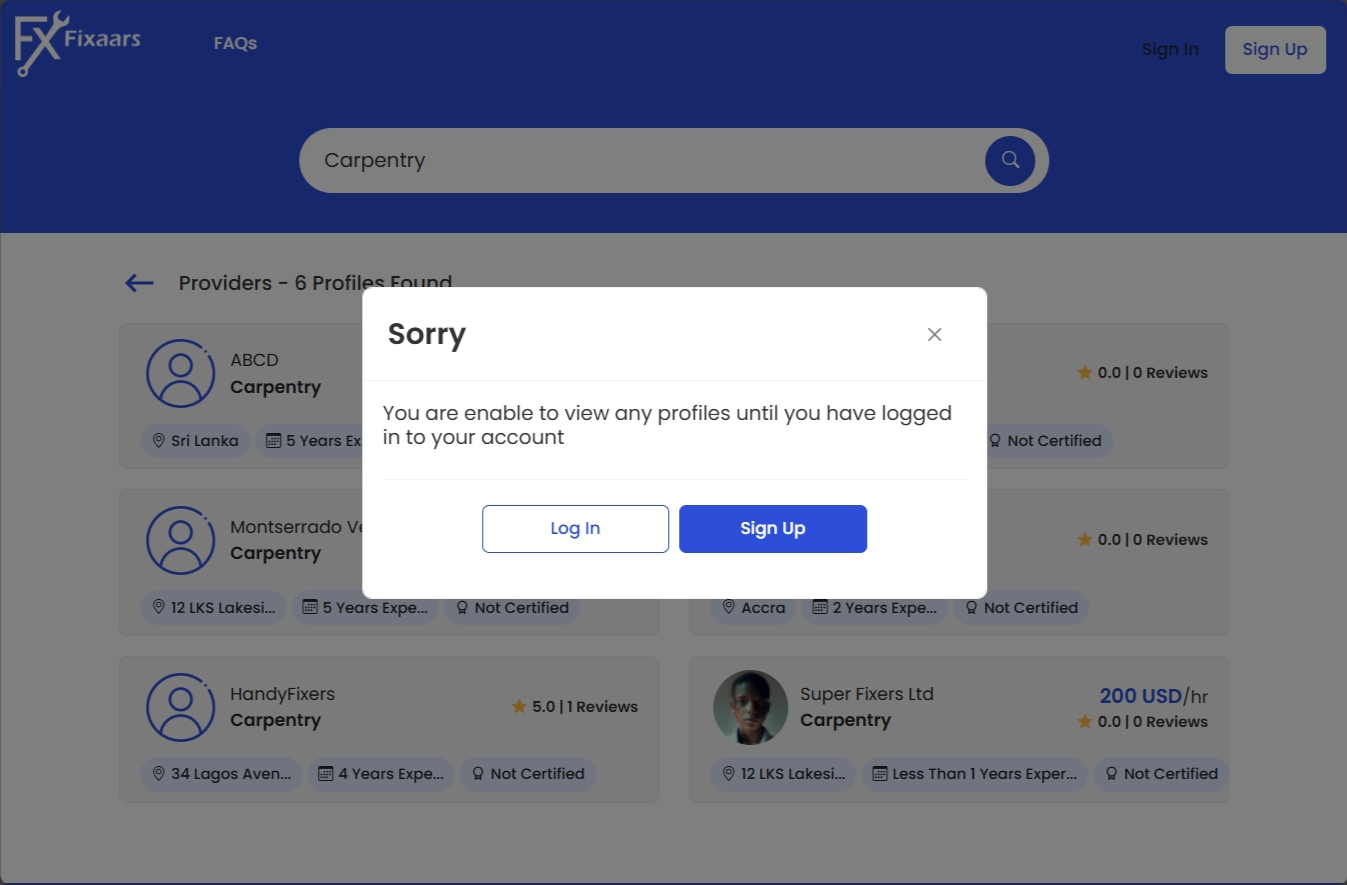
\includegraphics[width=12cm]{assets/demo/search-2.png}
\end{center}
\caption{Page de Recherche - Invité}
\end{figure}

Voici la page qui montre les détails d'un prestataire de services :

\vspace{0.35cm}
\begin{figure}[H]
\begin{center}
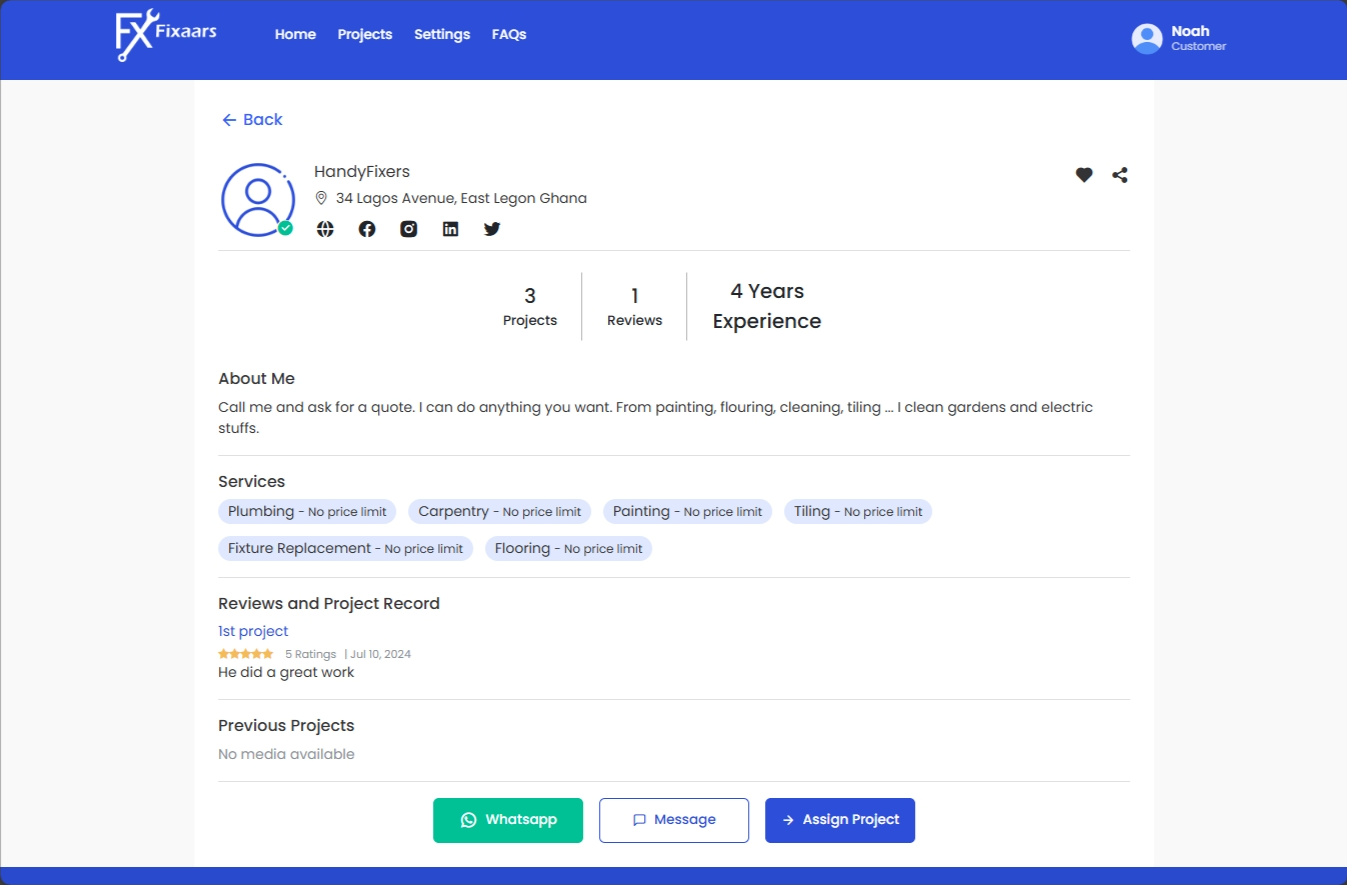
\includegraphics[width=12cm]{assets/demo/search-profile.png}
\end{center}
\caption{Page de Recherche - Profile}
\end{figure}

Après, l'utilisateur peut choisir d'engager directement le professionnel sur WhatsApp ou l'écrire via l'outil de communication intégré. Il peut tout aussi bien assigner le projet au prestataire. 


\subsection{Création \& Gestion de Projet}

Après avoir trouvé un prestataire de service, l'utilisation peut créer un projet. Dans le processus de création de projet il doit spécifier les informations initiales du projet 


\vspace{0.35cm}
\begin{figure}[H]
\begin{center}
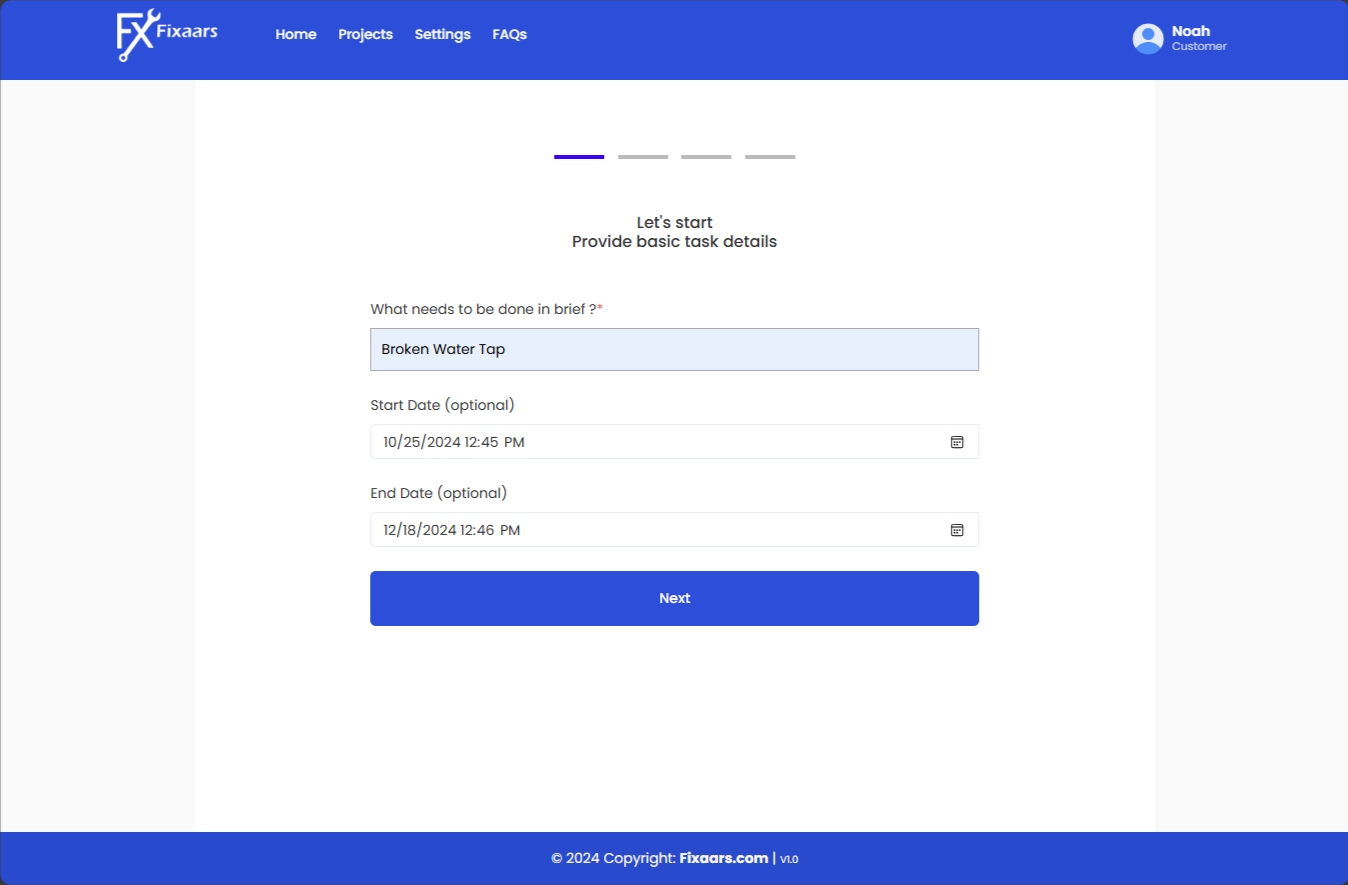
\includegraphics[width=12cm]{assets/demo/setup-1.png}
\end{center}
\caption{Creation de projet - 1/4}
\end{figure}

Puis ensuite il peut spécifier la localisation, l'adresse à laquelle il aimerait accueillir le prestataire.

\vspace{0.35cm}
\begin{figure}[H]
\begin{center}
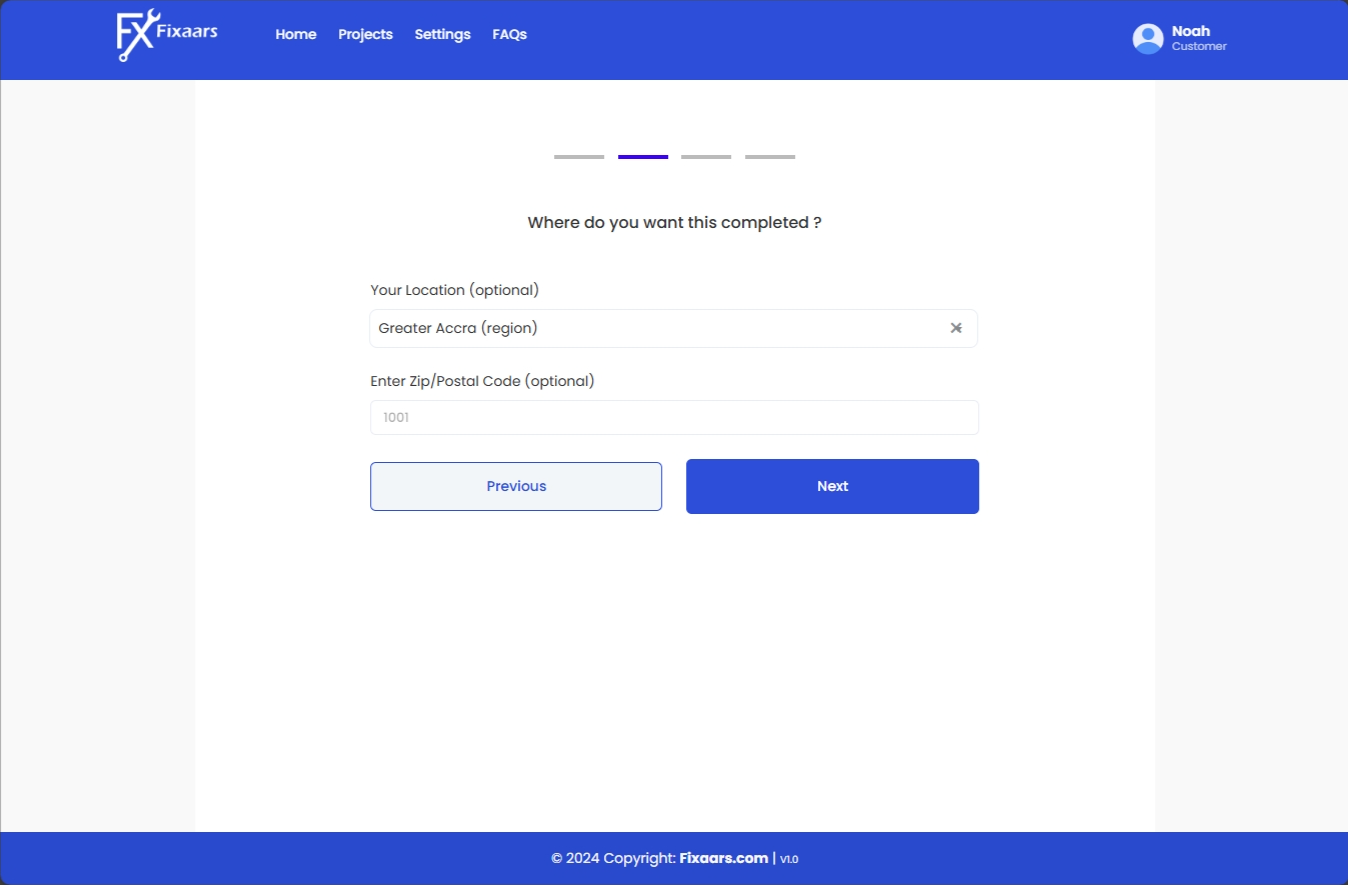
\includegraphics[width=12cm]{assets/demo/setup-2.png}
\end{center}
\caption{Creation de projet - 2/4}
\end{figure}

Après il peut ajouter plus de détails au projet, ou même y joindre des fichiers médias.

\vspace{0.35cm}
\begin{figure}[H]
\begin{center}
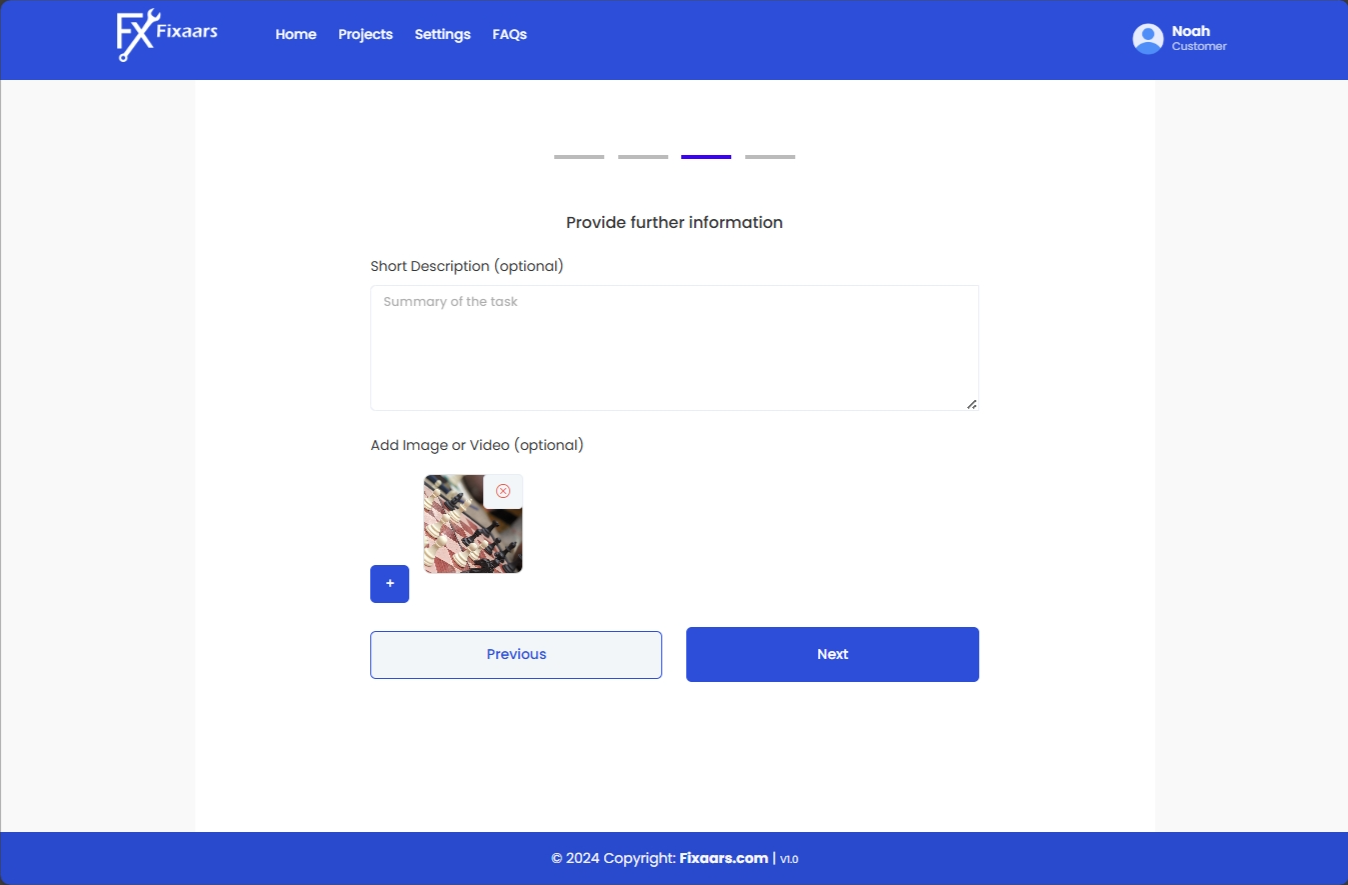
\includegraphics[width=12cm]{assets/demo/setup-3.png}
\end{center}
\caption{Creation de projet - 3/4}
\end{figure}

Enfin , il peut spécifier le budget dont il dispose.

\vspace{0.35cm}
\begin{figure}[H]
\begin{center}
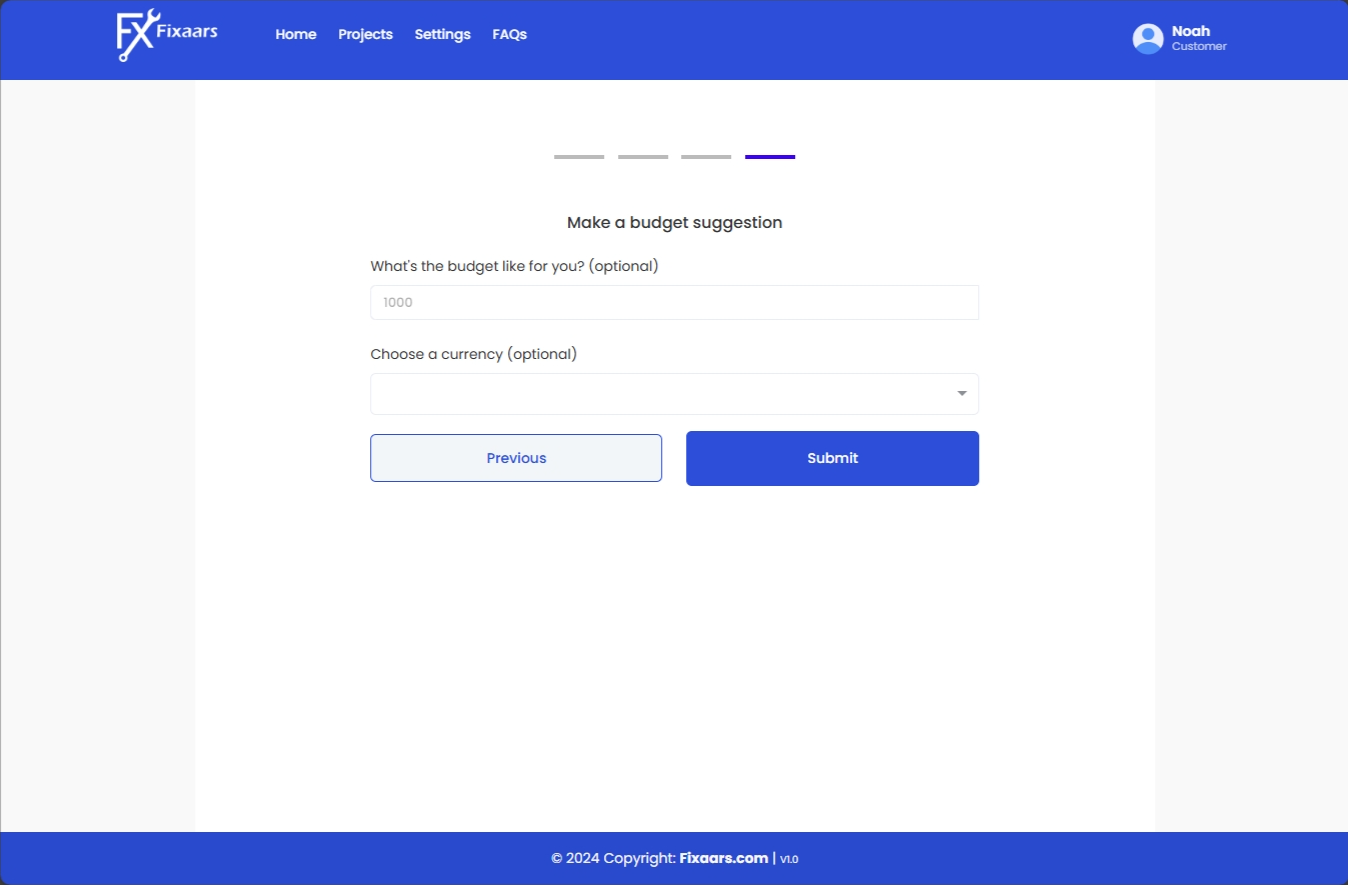
\includegraphics[width=12cm]{assets/demo/setup-4.png}
\end{center}
\caption{Creation de projet - 4/4}
\end{figure}

Le prestataire de service verra ce projet dans sa liste de projet en attente et pourra accepter ou refuser. 

\vspace{0.35cm}

Voici comment se présente la page de gestion de projets 

\vspace{0.35cm}
\begin{figure}[H]
\begin{center}
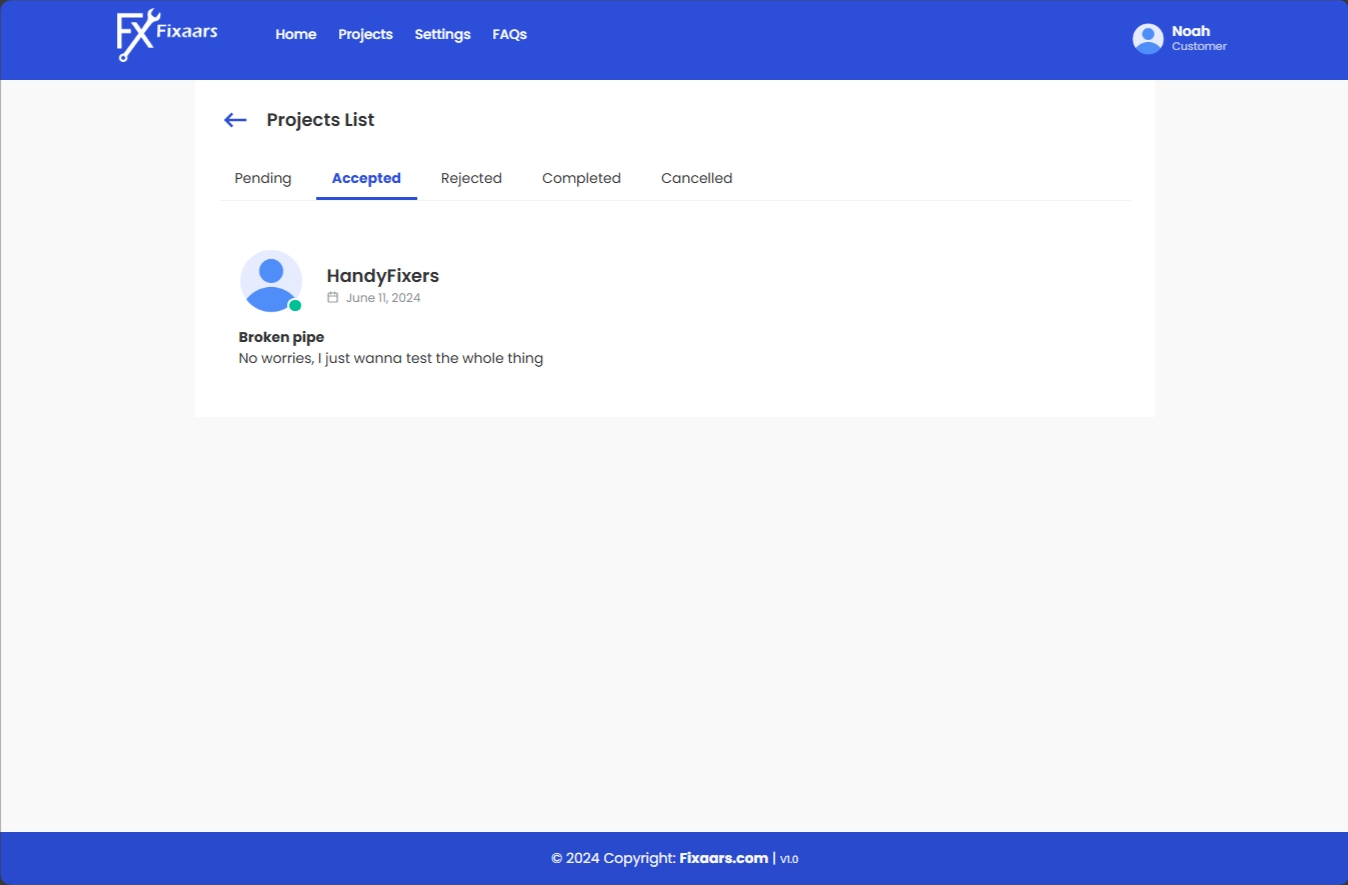
\includegraphics[width=12cm]{assets/demo/pj-list.png}
\end{center}
\caption{Gestion de Projets}
\end{figure}

\subsection{Module de chat, messages en temps réel et appels audio \& video}

Cette partie permet au prestataire et au responsable de projets de communiquer aisément sur la plateforme.

Les deux utilisateurs peuvent en effet : 

\begin{description}
    \item[- S'échanger des messages textuels] :

\vspace{0.35cm}
\begin{figure}[H]
\begin{center}
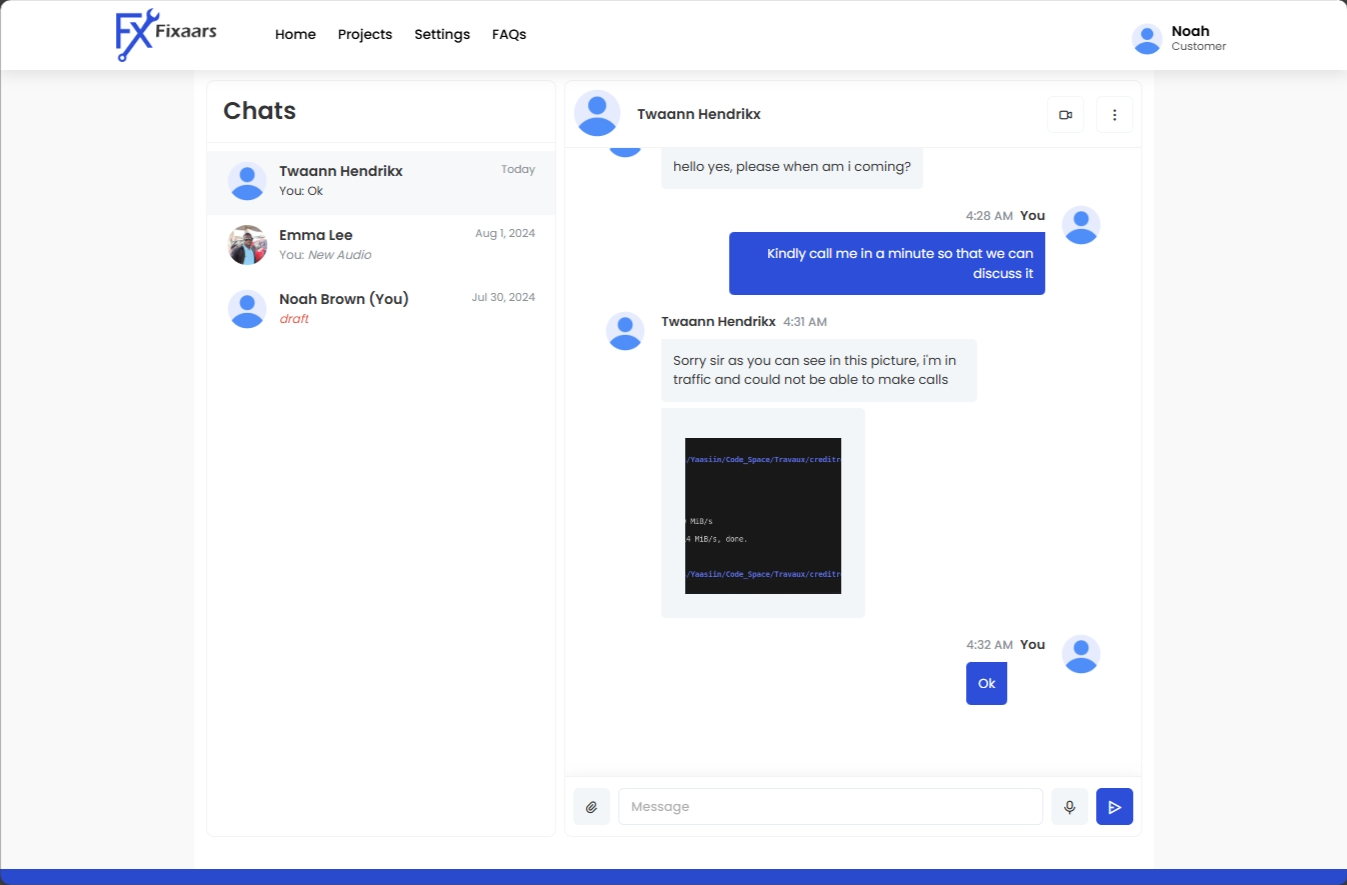
\includegraphics[width=12cm]{assets/demo/chat-1.png}
\end{center}
\caption{chat : Envoi de message textuels en temps réel}
\end{figure}

    \item [- Enregistrer des notes vocales ou envoyer des pièces jointes] : 

\vspace{0.35cm}
\begin{figure}[H]
\begin{center}
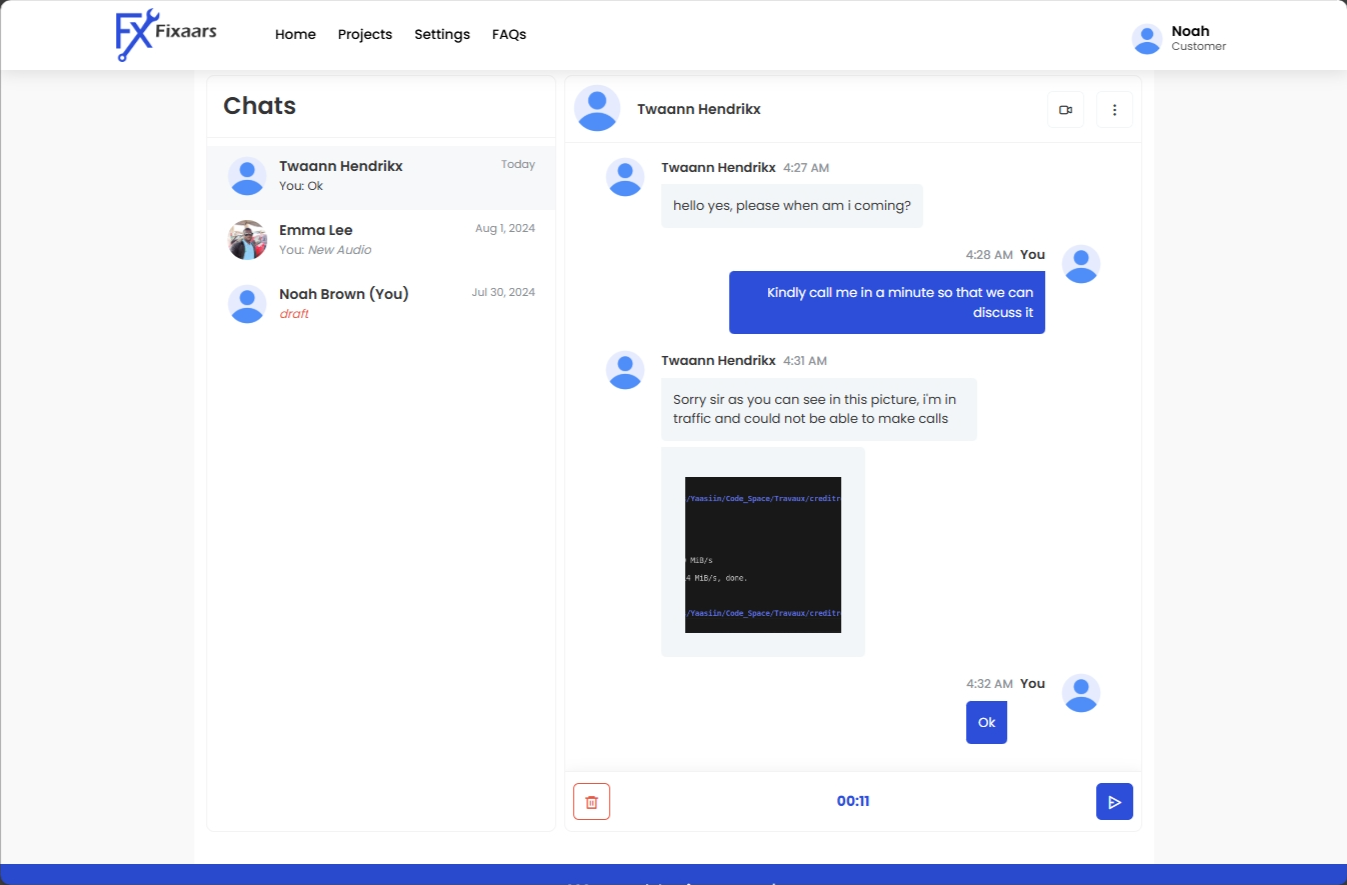
\includegraphics[width=12cm]{assets/demo/chat-2.png}
\end{center}
\caption{chat : Notes Vocales \& Pièces jointes}
\end{figure}

    \item[- Appeler ou Recevoir des appels audio ou videos] :

\vspace{0.35cm}
\begin{figure}[H]
\begin{center}
\includegraphics[width=12cm]{assets/demo/chat-3.png}
\end{center}
\caption{chat : Notification d'appel}
\end{figure}

    \item[- Disposer d'un temps d'appel illimité] : Les utilisateurs peuvent communiquer sans restriction de temps en video ou audio, en temps réel

\vspace{0.35cm}
\begin{figure}[H]
\begin{center}
\includegraphics[width=12cm]{assets/demo/chat-4.png}
\end{center}
\caption{chat : Appel video en cours}
\end{figure}
\end{description}


\section{Déroulement du projet - Tâches et Réalisations}

Mon stage à JS Morlu Ghana a débuté le 29 janvier 2024. Durant le déroulement du stage, plusieurs tours de révisions des spécifications du projet ont eu lieu. Cela a conduit à des réajustements non seulement sur l'implémentation des fonctionnalités prévues initialement, mais aussi sur l'équipe de développement associée au projet. Voici un rapport chronologique des tâches que j'ai effectuées à JS Morlu Ghana tout au long de la période de stage dans le cadre du projet Fixaars :

\subsection*{De Janvier à Fevrier} 

Cette période a consisté principalement à recueillir le plus d'informations sur le projet et à préparer la codebase du projet avec les modules minimums. Mes tâches ont consisté en ce qui suit :\\ 

\begin{itemize}
    \item \textbf{Onboarding sur le projet} : Initiation à la stack de gestion de projet interne de l'entreprise, Reajustement des specifications, Modelisation et début d'Analyse prévisionnelle du projet
    \item \textbf{Initialisation} : Mise en place de l'architecture du projet avec des fonctionnalités d'authentification côté backend. Implémentation de l'autorisation RBAC (Role Based Access Control), Début intégration du template pour le backoffice (partie Administrateur)
    \item \textbf{ Backoffice - Implémentation des CRUD} : Mise en place des fonctionnalités de créations, Lecture, Modification et suppressions des entités du package \textit{Catalog} côté admin.
    \item \textbf{Implementation Minimale de la vue utilisateur} : Mise en place du module responsable de la gestion de Projets sur la plateforme.
\end{itemize}

\vspace{1cm}
Nous avons très vite avancé durant le premier mois du projet. Sur papier, une grande partie des fonctionnalités du projet a été implémentée en un rien de temps, mais dans le fond, il y avait beaucoup de choses que je n'avais pas encore très bien assimilées sur le projet. Cette rapidité dans l'implémentation était due au fait que nous nous inspirions d'une plateforme existante (\href{https://www.thumbtack.com/}{Thumbtack}) dont l'idée était similaire au projet que nous réalisions.

\subsection*{De Fevrier à Mars}

\begin{itemize} 
    \item Avancée fulgurante sur le module chargée de la gestion de projets. J'ai implémenté un Kanban board permettant aux service seekers de gérer les projets auquels il assignent le service provider.
    \item J'ai implémenté les fonctionnalités de recherches de services providers : Recherche par services proposés, filtrage par emplacement, filtrage par options, Geolocalisation avec OpenStreetMap.
\end{itemize}

\vspace{1cm}
Les principales difficultés dans cette partie consistaient en l'implémentation du kanban board pour la gestion de projet. Au fur et à mesure que les fonctionnalités côté utilisateur étaient faites, j'itérais immédiatement sur la partie backoffice pour que l'admin puisse gérer les entités créées. Cette flexibilité a été rendue possible grâce à l'utilisation des datatables. Le superviseur avait mis un point d'honneur sur l'implémentation d'une fonction de mapping des données de n'importe quel type directement au backend avec le mécanisme d'affichage des datatables.

\subsection*{De Mars à Avril}

Durant cette période du stage, après plusieurs réunions et présentations avec l'équipe impliquée dans le projet, des changements notables ont été apportés sur plusieurs processus du projet. Beaucoup de fonctionnalités déjà implémentées ont été touchées. La principale tâche de cette période a été la mise à jour de la codebase en intégrant les différents changements. \\

\begin{itemize}
    \item \textbf{Restructuration des rôles utilisateurs} : désormais deux comptes distincts sont à considérer, un service seeker et un service provider. Ceci n'était pas le cas dans la version précedente. Initialement un utilisateur était libre de chercher et d'offrir des services en utilisant un et un seul compte.
    \item \textbf{Ajout des données géographiques} (Pays, Regions, Villes, Quartiers ...)
    \item \textbf{Changement du business process} : 
    J'ai fait la mise à jour du modele et des différents services et apis. J'ai modifier le processus d'authentification des utilisateurs, J'ai retiré la gestion de projets (Kanban).
    \item \textbf{Authentification des réseaux Sociaux (Social Authentication)} : J'ai implémenté l'authentification utilisant les différents comptes et réseaux sociaux (Google, Facebook, LinkedIn)
\end{itemize}

\vspace{1cm}
Cette période a été particulièrement coûteuse durant toute la durée du stage. Le changement du processus utilisateur a eu des répercussions sur presque toutes les couches du logiciel. J'ai donc refait l'intégration des nouvelles fonctionnalités en supprimant celles qui ont été abandonnées.

\subsection*{De Avril à Mai}

L'objectif de cette période était de produire une version minimale comprenant les feedbacks récoltés auprès de l'équipe et d'en faire une démo aux utilisateurs finaux du système. Dans ce sens, un nouveau développeur a été ajouté au projet et a endossé la responsabilité du frontend. Cette restructuration m'a permis d'avancer rapidement dans l'implémentation des nouvelles fonctionnalités.\\

\begin{itemize}
    \item \textbf{Mise en place du serveur de test, déploiement et Mise à jour de la documentation postman}  pour facilliter la collaboration
    \item \textbf{Authentification des réseaux Sociaux} : J'ai implémenté l'authentification utilisant les différents comptes et réseaux sociaux (Google, Facebook, LinkedIn)
    \item \textbf{Ajout de la messagerie instantannée} : J'ai implémenté la fonctionnalité de discussion instantannées avec Socket.io aussi bien côté backend que frontend.
\end{itemize}
\vspace{1cm}

A l'issue de cette période, une version minimale du logiciel a été présentée aux utilisateurs finaux du système. Nous avons récolté des retours et des suggestions sur les fonctionnalités du système. 
Cette période m'a aussi permis d'apprendre une nouvelle technologie (la communication par sockets) nécessaire pour les systèmes en temps réel. 

\subsection*{De Mai à Juin}

\begin{itemize}
    \item \textbf{Optimisation du chat instantannée} : J'ai implémenté la fonctionnalité d'appel audio/video utilisant Peer.JS\footnote{Voir annexes}, Ajouté le support d'envoi de fichiers media et des notes vocales. 
    \item \textbf{Implémentation de la pipeline CI/CD} : J'ai mis en place la pipeline CI/CD avec bitbucket-ci permettant de mettre à jour le déploiement à chaque fois que l'on merge sur le master.
    \item \textbf{Gestion des offres\footnote{initialement Gestion de Projets}} : J'ai ajouté les apis responsables de l'acceptation, l'annulation et la completion d'une offre, 
\end{itemize}

\subsection*{De Juin à Juillet}

Cette période marquait progressivement la fin du stage et représentait une phase cruciale pour garantir la qualité et la stabilité du projet. Elle a consisté principalement en la \textbf{révision des fonctionnalités} par le testeur QA (Assurance Qualité). Ce processus impliquait une série de tests rigoureux, notamment :  

\begin{itemize}
    \item \textbf{Tests fonctionnels} : Vérification de chaque fonctionnalité pour s'assurer qu'elle répond aux exigences définies dans les spécifications initiales.
    \item \textbf{Tests de compatibilité} : Validation de l'application sur différents navigateurs, systèmes d'exploitation ou appareils, selon les besoins du projet.  
    \item \textbf{Tests de régression} : Identification de potentiels effets secondaires introduits par les récents correctifs ou mises à jour.  
\end{itemize}

Au cours de cette phase, des \textbf{rapports détaillés de bugs} et des dysfonctionnements ont été générés par le testeur QA, puis partagés avec l'équipe de développement via la plateforme \textbf{JIRA}. En collaboration avec le testeur, j’ai également participé à l’analyse et à la correction de certaines de ces anomalies, en veillant à ce que les modifications apportées n’altèrent pas d’autres parties du système.

\section{Difficultés rencontrées et Apports du stage}

\subsection*{Difficultés}

Au cours de ce stage, j’ai eu à rencontrer plusieurs difficultés. La toute première difficulté fut au niveau de l'analyse prévisionnelle du projet. J'ai eu du mal à concevoir le projet sur une durée réaliste. L'assistance du maître de stage dans cette partie fut la bienvenue. \\

Les autres difficultés rencontrées furent principalement d'ordre technique. En premier lieu, j'ai éprouvé des \textbf{difficultés à intégrer les fonctionnalités de discussions instantanées avec Socket.IO}, bien que j’aie une connaissance préalable du concept grâce à son utilisation dans un projet récent. Ces problèmes ont été particulièrement coûteux en termes de temps, car les subtilités de l'implémentation et la gestion des événements en temps réel dans un environnement complexe se sont révélées plus ardues que prévu.

Pour surmonter ces obstacles, j'ai entrepris une \textbf{veille technologique rapide}, en suivant un cours pratique intitulé \textit{\href{https://www.linkedin.com/learning/node-js-real-time-web-with-socket-io}{``Node.js: Real-Time Web with Socket.IO''}} disponible sur LinkedIn Learning. Ce cours m’a permis de renforcer mes bases sur les interactions en temps réel et de découvrir de nouvelles bonnes pratiques pour structurer mon code avec Socket.IO.

De plus, j’ai consacré un temps significatif à explorer en profondeur la \textbf{documentation officielle de Socket.IO} (\href{https://socket.io/docs/v3}{Socket.IO Docs}\footnote{Socket.IO Docs : \href{https://socket.io/docs/v3}{https://socket.io/docs/v3}}), où j’ai étudié les différentes fonctionnalités offertes par cet outil, notamment :  
\begin{itemize}
    \item La gestion des connexions multiples et des déconnexions.
    \item L’utilisation des \textit{namespaces} et des \textit{rooms} pour structurer les échanges en fonction des besoins spécifiques de l’application.
    \item La gestion des erreurs pour assurer la résilience des interactions en cas de problèmes réseau.
\end{itemize}

Cette expérience a renforcé mes compétences en temps réel et m’a appris l’importance d’une \textbf{approche méthodique face aux outils nouveaux ou complexes}, en combinant apprentissage théorique et expérimentation pratique. \\

Aussi, lors de la mise en place du déploiement, j'ai été confronté à une erreur liée au mécanisme CORS (Cross-Origin Resource Sharing), qui empêchait certaines requêtes effectuées par le frontend d’accéder aux ressources exposées par le backend. Cette difficulté est survenue lorsque l’application était testée dans un environnement de test (en ligne), où les restrictions de sécurité liées aux requêtes inter-origines sont strictement appliquées par les navigateurs.\\

En effet, CORS, pour Cross-Origin Resource Sharing, est un mécanisme de sécurité utilisé par les navigateurs pour contrôler les requêtes HTTP effectuées entre différentes origines. Une origine est définie par le trio :

\begin{itemize}
    \item Protocole (\textit{exemple :} http:// ou https://),
    \item Nom de domaine (\textit{exemple :} fixaars.com),
    \item Port (\textit{exemple :} :80 ou :3000).
\end{itemize}

Après plusieurs essais infructueux pour identifier la cause exacte du problème auquel je me heurtais, j'ai procédé à :

\begin{itemize}
    \item Examiner les configurations du serveur backend, notamment les en-têtes HTTP Access-Control-Allow-Origin et les autres paramètres liés aux règles CORS.
    \item Consulter les logs du serveur pour repérer les requêtes bloquées et mieux comprendre la source de l’erreur.
    \item Analyser les différences entre l'environnement local et celui de production, ce qui m’a permis de réaliser que certains domaines autorisés étaient mal configurés ou manquaient dans les paramètres de production.
\end{itemize}

Pour résoudre le problème, j'ai mis en place une configuration CORS plus flexible et sécurisée en :

\begin{itemize}
    \item Autorisant uniquement les domaines spécifiques du frontend à accéder aux ressources.
    \item Restreignant les méthodes HTTP et les en-têtes autorisés à ceux nécessaires pour l'application.
    \item Testant de bout en bout les requêtes pour m'assurer que les ajustements apportés n'introduisaient pas de nouvelles vulnérabilités.
\end{itemize}

Cette difficulté a été une opportunité d'apprentissage, car elle m'a permis de mieux comprendre le fonctionnement des politiques de sécurité des navigateurs et l’importance d’un déploiement rigoureux.

\subsection*{Apports}
Ce stage m'a beaucoup appris. C'était une expérience enrichissante que de travailler dans un environnement structuré et collaboratif, en utilisant la \textbf{méthodologie Agile}. Cette approche m’a permis de mieux comprendre l’importance de la communication, de l’adaptabilité et des cycles de développement itératifs dans la gestion de projets logiciels.

Un apport majeur a été l’opportunité d’approfondir mes compétences techniques en abordant des outils et technologies que je ne maîtrisais pas entièrement auparavant. Par exemple, l'intégration de \textbf{socket.io} pour les discussions en temps réel et la gestion des \textbf{CORS} m'ont non seulement permis de renforcer mes bases techniques, mais également d'améliorer ma capacité à résoudre des problèmes complexes grâce à la documentation, aux ressources en ligne, et à la collaboration avec l'équipe.

En outre, travailler dans une équipe multidisciplinaire m'a enseigné l'importance de la collaboration interfonctionnelle. En interagissant avec des profils variés tels que des testeurs QA, des designers et des responsables produits, j’ai appris à mieux comprendre leurs besoins et à adapter mon travail en conséquence pour garantir un produit final cohérent et aligné avec les attentes.

Sur le plan personnel, ce stage m’a permis de développer des \textbf{compétences clés en gestion du temps et en organisation}, notamment en jonglant avec des deadlines serrées et des priorités fluctuantes. Enfin, cette expérience m'a conforté dans mon envie de poursuivre une carrière dans le développement logiciel, en m’aidant à identifier mes forces et les axes sur lesquels je souhaite continuer à progresser.

\newpage
\newpage

\chapter*{Conclusion Générale}
Ce stage chez JS Morlu a été une étape enrichissante dans mon parcours professionnel. J'ai eu l'opportunité de travailler sur un projet concret et innovant, Fixaars, qui répond à un besoin réel de la communauté locale au Ghana. J'ai pu mettre en pratique mes compétences techniques, développer de nouvelles compétences professionnelles et découvrir le monde du travail dans une entreprise internationale. Je suis particulièrement fier d'avoir contribué à la création de l'application Fixaars, qui permettra aux utilisateurs de trouver plus facilement des prestataires de services qualifiés et de bénéficier de services de qualité. Je suis également reconnaissant envers JS Morlu et mon superviseur, M. Aliloulaye Tchaou, pour m'avoir donné cette opportunité et pour m'avoir accompagné tout au long de mon stage. Cette expérience a confirmé mon intérêt pour le développement d'applications mobiles et m'a donné envie de poursuivre ma carrière dans ce domaine. Je suis convaincu que les compétences et les connaissances que j'ai acquises pendant ce stage seront un atout précieux pour mon avenir professionnel. Je suis impatient de relever de nouveaux défis et de continuer à apprendre et à me développer dans le monde de l'informatique.
}

%Ne pas numéroter cette partie
\part*{Annexes}
%Rajouter la ligne "Annexes" dans le sommaire
\addcontentsline{toc}{part}{Annexes}

\appendix

% {\fontsize{18pt}{18pt}\selectfont

\chapter*{Annexe : Implémentation du Module de Chat}
\addcontentsline{toc}{chapter}{Implémentation du Module de Chat}
\markboth{Implémentation du Module de Chat}{Implémentation du Module de Chat}

%changer le format des sections, sections pour apparaittre sans le num de chapitre
\makeatletter
\renewcommand{\thesection}{\@arabic\c@section}
\makeatother

%recommencer la numérotation des section à "1"
\setcounter{section}{0}

Cette annexe présente les détails sur l'implémentation d'une fonctionnalité en particulier : le système de chat.

\vspace{0.35cm}

Pour constituer le module de chat nous avons utilisé les technologies Socket.io , peerjs.

Dans ce projet, l'implémentation combine deux paradigmes de communication : \verb|REST API| et \verb|WebSocket| avec Socket.io.

\begin{itemize}
    \item  \verb|REST API (Representational State Transfer)| est un style architectural pour les services web qui repose sur des requêtes HTTP classiques. Ce paradigme suit un modèle \textbf{stateless}, où chaque requête est indépendante et doit contenir toutes les informations nécessaires pour son traitement. Les \textbf{REST API} sont utilisées pour gérer des échanges de données simples, comme la récupération ou la modification d'informations sur le serveur.
    \item \verb|WebSocket|, quant à lui, est un protocole de communication bidirectionnelle qui permet d'établir une connexion persistante entre le client et le serveur. Contrairement aux requêtes HTTP classiques, \textbf{WebSocket} permet au serveur d'envoyer des données au client de manière instantanée sans que ce dernier n'ait besoin de faire une nouvelle requête. Ce paradigme est idéal pour les applications nécessitant des mises à jour en temps réel, telles que les chats, les notifications ou les jeux multijoueurs. \textbf{Socket.io} est une bibliothèque JavaScript qui facilite l'implémentation de \textbf{WebSocket} et permet de gérer les événements en temps réel entre le serveur et le client.
\end{itemize}

\vspace{0.35cm}

D'une part, nous utilisons REST API pour gérer les échanges classiques de données entre le client et le serveur, permettant ainsi de manipuler les ressources de manière stateless via des requêtes HTTP standard. Ce modèle est idéal pour les opérations simples telles que la récupération d'informations ou la gestion d'entités.

\vspace{0.35cm}

D'autre part, Socket.io est intégré pour les fonctionnalités nécessitant une communication en temps réel. Grâce à sa capacité à maintenir des connexions persistantes et bidirectionnelles, Socket.io facilite la gestion des événements en temps réel, tels que les notifications, les chats en direct, ou les mises à jour instantanées. Cette approche hybride permet de tirer parti des avantages de chaque technologie selon les besoins spécifiques de l'application.

\clearpage

\section{Module de Chat - Implémentation Côté Backend}

La première étape côté backend a consisté à établir les tables selon le diagramme de classes présenté plus haut à la \autoref{subsection_package_communication}. Cette implémentation repose sur l'architecture présentée à la \autoref{architecture_backend} plus haut.

Les extraits de code ci-dessous permettent l'implémentation des classes essentielles.


\begin{figure}[H]
    \centering
    \includegraphics[width=16cm]{assets/annexes/snippet.png}
    \caption{Code pour implémenter la classe attachement avec Typeorm}
\end{figure}

\begin{figure}[H]
    \centering
    \includegraphics[width=13.5cm]{assets/annexes/snippet (1).png}
    \caption{Code pour implémenter la classe message avec Typeorm}
\end{figure}

\begin{figure}[H]
    \centering
    \includegraphics[width=16cm]{assets/annexes/snippet (2).png}
    \caption{Code pour implémenter la classe call avec Typeorm}
\end{figure}

\begin{figure}[H]
    \centering
    \includegraphics[width=13.5cm]{assets/annexes/snippet (3).png}
    \caption{Code pour implémenter la classe room avec Typeorm}
\end{figure}

\clearpage

Après avoir implémenté le modèle, la prochaine étape consiste à développer les services qui utiliseront ces modèles. Dans ce projet, nous avons mis en place deux classes de services essentielles.

\begin{description}
    \item[- Service de gestion des salons (RoomService)] : Cette classe contient trois méthodes principales :
        \begin{enumerate}
            \item \verb|findChatRooms| : récupère tous les salons de discussion associés à l'utilisateur qui effectue la requête.
            \item \verb|findOrCreateChatRoom| : recherche un salon existant entre deux utilisateurs ou en crée un nouveau si aucun n'existe.
            \item \verb|addMessage| : ajoute un message à un salon de discussion existant.
        \end{enumerate}
        
    \item[- Service de gestion des messages (\textbf{MessageService})] : Ce service gère l'envoi et la récupération des messages dans une conversation :
        \begin{enumerate}
            \item \verb|findByChatRoomId| : récupère tous les messages d'un salon de discussion donné, en incluant les informations des utilisateurs, rôles et pièces jointes.
            \item \verb|newMessage| : crée un nouveau message en associant l'utilisateur, le salon de discussion et les éventuelles pièces jointes.
        \end{enumerate}
\end{description}

\vspace{0.35cm}

Après avoir implémenté ces services, on peut désormais passer à l'implémentation de la classe responsable des connexions instantannées. 

\vspace{0.35cm}

Commençons d'abord à initialiser la classe. 

\clearpage

\begin{figure}[H]
    \centering
    \includegraphics[width=16cm]{assets/annexes/snippet (4).png}
    \caption{Socket Handler - Définition de la classe et du constructeur}
\end{figure}

\vspace{1cm}

Ensuite, nous devons définir la méthode responsable de gérer la connexion du socket. Cette méthode vérifie si l'utilisateur est authentifié puis elle monte les évenements avec les différents handlers de chaque évenement. 
Elle charge ensuite la liste des salons ou conversations concernant l'utilisateur et la retourne grâce à un évenement émis.

\begin{figure}[H]
    \centering
    \includegraphics[width=16cm]{assets/annexes/snippet (5).png}
    \caption{Socket Handler - Gestionnaire de Connexions}
\end{figure}

\vspace{1cm}

Après nous allons définir la méthode responsable de vérifier l'authentification des requêtes puis définir la fonction (\verb|attachSocketEvents| qui monte les évenements avec les différents handlers de chaque évenements. La dernière étape sera de définir les différents handlers des évenements écoutés par notre serveur socket.

\begin{figure}[H]
    \centering
    \includegraphics[width=13cm]{assets/annexes/snippet (6).png}
    \caption{Socket Handler - Middleware d'authentification }
\end{figure}

\vspace{1cm}

\begin{figure}[H]
    \centering
    \includegraphics[width=13cm]{assets/annexes/snippet (7).png}
    \caption{Socket Handler - Fonction AttachSocketEvents}
\end{figure}

\vspace{1cm}

\begin{figure}[htp]
  \centering
  \subfloat{\label{fig:first}\includegraphics[width=7.3cm, height=10.7cm]{assets/annexes/snippet (9).png}}
  ~
  \subfloat{\label{fig:second}\includegraphics[width=7.3cm]{assets/annexes/snippet (10).png}}
  ~\\
    \subfloat{\label{fig:third}\includegraphics[width=7.3cm]{assets/annexes/snippet (11).png}}
  ~
  \subfloat{\label{fig:fourth}\includegraphics[width=7.3cm, height=13.4cm]{assets/annexes/snippet (12).png}}
  \caption{Socket Handler - Fonctions Handlers}
  \label{fig:gallerieSockets}
\end{figure}

\clearpage

\vspace{1cm}

Une fois que cette classe est implémentée, nous devons la monter dans le point d'entrée de l'application (\verb|app.bootstrap.ts|.). Ci-dessous un exemple du code du fichier \verb|app.bootstrap.ts|

\vspace{0.35cm}

\begin{figure}[H]
    \centering
    \includegraphics[width=15cm]{assets/annexes/snippet (13).png}
    \caption{ Exemple du point d'entrée de l'application}
\end{figure}

Ceci marque la dernière étape d'implémentation au backend. La prochaine étape consiste à implémenter la fonctionnalité côté frontend. 

\section{Module de Chat - Implémentation Côté Frontend}

L'implémentation côté frontend nécessite qu'on fasse dans un premier temps la structure HTML et CSS du chat. Pour les besoins de ce rapport, et afin d'éviter de faire un développement trop grand, nous allons survoler cette partie et mettre un accents sur les parties clées de l'implémentation frontend. La structure est de telle qu'elle est incluse dans un conteneur principal avec une classe \verb|main-content| et fond gris clair. Il contient une zone de chat principale qui se structure en deux colonnes flexibles :

\begin{enumerate}
    \item \textbf{La liste des conversations} (Panneau gauche) avec une liste déroulante des utilisateurs et un système d'onglets pour chaque conversation
    \item \textbf{Zone de conversation active} (Panneau droit) . Il se subdivise en plusieurs zone : 
    \begin{itemize}
        \item \textbf{En-tête de conversation} :contient l'avatar de l'utilisateur, le nom et le statut avec des boutons d'action (appel video, menu dropdown contenant des boutons profile et report, bouton de fermeture du chat)
        \item \textbf{Zone de message} : C'est un conteneur de liste non ordonnée de composants messages générés par javascript
        \item \textbf{Barre d'outil inférieurs} : Contient le bouton pour les pièces jointes, la zone de saisie de message, les boutons de fonctionnalité audio (enregistrement , timer, suppression d'enregistrement),
        bouton d'envoi de message
    \end{itemize}
\end{enumerate}

\vspace{0.35cm}

En plus de tout ce qui a été décrit, cette page définit aussi des composants modaux pour la gestion des appels (Modal d'appel entrant ou sortant, Modal d'appel en cours).

\vspace{0.35cm}

Notre structure au niveau des modules javascript inclu dans la page de chat se distingue en trois fichiers essentiels décrits ci-dessous : 

\begin{figure}[H]
    \centering
    \includegraphics[width=15cm]{assets/annexes/snippet (14).png}
    \caption{ Scripts de gestion du chat}
\end{figure}

Les points clés dans l'implémentation de javascript de cette partie du projet sont les suivants : 

\vspace{0.35cm}

\subsection*{Gestion de la Connexion aux Sockets}

Dès le chargement de l'application, une connexion WebSocket est établie. L'utilisateur s'authentifie et rejoint automatiquement son salon de discussion.

\begin{figure}[H]
    \centering
    \includegraphics[width=15cm]{assets/annexes/snippet (15).png}
    \caption{ Gestion des connexions aux sockets}
\end{figure}

\subsection*{Envoi et Réception de Messages}

Les messages sont envoyés lorsqu’un utilisateur appuie sur Entrée ou clique sur le bouton d'envoi :

\begin{figure}[H]
    \centering
    \includegraphics[width=15cm]{assets/annexes/snippet (16).png}
    \caption{ Envoi de message}
\end{figure}

À la réception d’un message, il est immédiatement affiché dans l’interface utilisateur :

\begin{figure}[H]
    \centering
    \includegraphics[width=15cm]{assets/annexes/snippet (17).png}
    \caption{ Affichage immédiat du message à la réception}
\end{figure}

\subsection*{Indicateur de Saisie (Typing Status)}

Lorsque l’utilisateur commence à écrire, un signal est envoyé aux autres participants du salon :

\begin{figure}[H]
    \centering
    \includegraphics[width=15cm]{assets/annexes/snippet (18).png}
    \caption{ Signal de saisie en cours}
\end{figure}

L'affichage est mis à jour pour informer les autres utilisateurs :

\begin{figure}[H]
    \centering
    \includegraphics[width=15cm]{assets/annexes/snippet (19).png}
    \caption{ Mise à jour de l'indicateur de saisie}
\end{figure}

\subsection*{Envoi et Réception de Fichiers}

Les utilisateurs peuvent partager des fichiers en les convertissant en Base64 avant de les envoyer via WebSockets.

\begin{figure}[H]
    \centering
    \includegraphics[width=15cm]{assets/annexes/snippet (20).png}
    \caption{ Envoi et Réception de Fichiers}
\end{figure}

\subsection*{Gestion des Appels Audio/Vidéo avec WebRTC - Initialisation de WebRTC}

Chaque utilisateur possède un peer ID unique généré avec PeerJS. Un serveur STUN est utilisé pour la traversée des NATs.

\begin{figure}[H]
    \centering
    \includegraphics[width=15cm]{assets/annexes/snippet (21).png}
    \caption{ Initialisation du serveur STUN}
\end{figure}

Lorsqu'un utilisateur est prêt à recevoir des appels, il enregistre son peer ID sur le serveur :

\begin{figure}[H]
    \centering
    \includegraphics[width=15cm]{assets/annexes/snippet (22).png}
    \caption{ Enregistrement de Peer ID}
\end{figure}

\subsection*{Réception d’un Appel}

Lorsqu'un appel entrant est détecté, une sonnerie est jouée et une modalité d’appel s’affiche :

\begin{figure}[H]
    \centering
    \includegraphics[width=15cm]{assets/annexes/snippet (23).png}
    \caption{ Réception d’un Appel}
\end{figure}

\subsection*{Passer un Appel}

L’utilisateur peut initier un appel audio ou vidéo en sélectionnant le type d’appel :

\begin{figure}[H]
    \centering
    \includegraphics[width=15cm]{assets/annexes/snippet (24).png}
    \caption{ Initiation d'un appel}
\end{figure}

Une connexion WebRTC est alors établie avec l’interlocuteur :

\begin{figure}[H]
    \centering
    \includegraphics[width=15cm]{assets/annexes/snippet (25).png}
    \caption{ Etablissement de la connexion WebRTC}
\end{figure}


\subsection*{Terminer un Appel}

À la fin de l’appel, les flux médias sont arrêtés et les interfaces sont mises à jour :

\begin{figure}[H]
    \centering
    \includegraphics[width=15cm]{assets/annexes/snippet (26).png}
    \caption{ Terminer un appel}
\end{figure}

\subsection*{Affichage Dynamique des Messages et Notifications}

Les messages sont affichés en temps réel avec les informations de l’auteur :

\begin{figure}[H]
    \centering
    \includegraphics[width=15cm]{assets/annexes/snippet (27).png}
    \caption{ Methode de construction du message de notification}
\end{figure}

L’utilisateur reçoit également une notification lorsqu’un nouveau message arrive :

\begin{figure}[H]
    \centering
    \includegraphics[width=15cm]{assets/annexes/snippet (28).png}
    \caption{ Réception de notification de message}
\end{figure}

\subsection*{Enregistrement et Envoi de Messages Audio}

Le système intègre une fonctionnalité d’enregistrement audio permettant aux utilisateurs d’envoyer des messages vocaux.

\vspace{0.35cm}

Lorsqu'un utilisateur clique sur le bouton d'enregistrement, l’application demande l'accès au microphone et démarre l’enregistrement via MediaRecorder.

\begin{figure}[H]
    \centering
    \includegraphics[width=15cm]{assets/annexes/snippet (29).png}
    \caption{ Démarrer l’Enregistrement}
\end{figure}

\begin{description}
    \item[Fonctionnalités implémentées par la méthode] :
    \begin{itemize}
        \item Envoi d’un signal de statut "Recording..." aux autres utilisateurs.
        \item Stockage des données audio sous forme de Blob.
        \item Masquage des éléments inutiles dans l'interface.
    \end{itemize}
\end{description}

\subsection*{Envoyer un Message Vocal}

Lorsque l'utilisateur termine l’enregistrement, le fichier est converti en Base64 et envoyé via Socket.io.

\begin{figure}[H]
    \centering
    \includegraphics[width=15cm]{assets/annexes/snippet (30).png}
    \caption{ Envoyer un Message Vocal}
\end{figure}

\begin{description}
    \item[Détails importants] :
    \begin{itemize}
        \item L’enregistrement est arrêté et converti en fichier Base64
        \item Le fichier est envoyé au serveur WebSocket
        \item L’interface est réinitialisée.
    \end{itemize}
\end{description}


\subsection*{Supprimer un Enregistrement}

L'utilisateur peut annuler un enregistrement avant l'envoi :

\begin{figure}[H]
    \centering
    \includegraphics[width=15cm]{assets/annexes/snippet (31).png}
    \caption{ Supprimer un Enregistrement}
\end{figure}

\subsection*{Gestion du Timer d’Enregistrement}

Un compteur de temps s'affiche pour indiquer la durée de l'enregistrement :

\begin{figure}[H]
    \centering
    \includegraphics[width=15cm]{assets/annexes/snippet (32).png}
    \caption{ Gestion du Timer d’Enregistrement}
\end{figure}


\subsection*{Mise à Jour Dynamique de l’Interface}

Lors de l'enregistrement ou de l'envoi, certains boutons sont cachés ou affichés :

\begin{figure}[H]
    \centering
    \includegraphics[width=15cm]{assets/annexes/snippet (33).png}
    \caption{ Mise à Jour Dynamique de l’Interface}
\end{figure}

%\chapter*{Annexe 2}
\addcontentsline{toc}{chapter}{Annexe 2}

%changer le format des sections, subsections pour apparaittre sans le num de chapitre
\makeatletter
\renewcommand{\thesection}{\@arabic\c@section}
\makeatother

%recommencer la numérotation des section à "1"
\setcounter{section}{0}



% }

%récupérer les citation avec "/footnotemark"
%\nocite{*}

%choix du style de la biblio
%\bibliographystyle{plain}
%inclusion de la biblio

%\bibliography{bibliographie.bib}
%voir wiki pour plus d'information sur la syntaxe des entrées d'une bibliographie

\end{document}

